\documentclass[journal=jcisd8,manuscript=article]{achemso}

\usepackage[T1]{fontenc}
\usepackage{amsmath}
\usepackage{booktabs}
\usepackage{graphicx}
\usepackage{longtable}
\usepackage{array}
\renewcommand{\thetable}{S\arabic{table}}
\renewcommand{\thefigure}{S\arabic{figure}}
\renewcommand{\topfraction}{0.9}
\renewcommand{\bottomfraction}{0.9}
\renewcommand{\textfraction}{0.05}
\renewcommand{\floatpagefraction}{0.6}
\setcounter{topnumber}{3}
\setcounter{bottomnumber}{3}
\setcounter{totalnumber}{5}

\setlength{\emergencystretch}{3em}
\newcommand{\TBD}[1]{\textbf{[#1]}}
\newcommand{\dS}{\Delta S}
\newcommand{\kcal}{kcal\,mol$^{-1}$}
\IfFileExists{numbers.tex}{% Generated by make_numbers.py; do not edit.
\newcommand{\addLigandSd}{0.87}
\newcommand{\addRawSd}{1.20}
\newcommand{\addTargetSd}{0.51}
\newcommand{\addVarShare}{70}
\newcommand{\ceilLig}{0.84}
\newcommand{\contactMany}{0.43}
\newcommand{\contactNone}{0.31}
\newcommand{\controlNoContact}{0.18}
\newcommand{\dockTwelveEdits}{3{,}072}
\newcommand{\dockTwelveEditsTwentyfour}{73{,}728}
\newcommand{\dsigmaMed}{0.26}
\newcommand{\editsAllMean}{22}
\newcommand{\editsLeftEight}{7}
\newcommand{\editsLeftFull}{18}
\newcommand{\editsLeftTwelve}{10}
\newcommand{\editsLeftTwo}{2}
\newcommand{\fracMulti}{41}
\newcommand{\fracNull}{8}
\newcommand{\fracSingle}{20}
\newcommand{\geoLooR}{0.09}
\newcommand{\nChangesKept}{274{,}295}
\newcommand{\nContactEdits}{1{,}007}
\newcommand{\nContactOf}{57}
\newcommand{\nContactTargets}{49}
\newcommand{\nDock}{305{,}227}
\newcommand{\nEdits}{1{,}233}
\newcommand{\nHeldTargets}{19}
\newcommand{\nNegSlope}{44}
\newcommand{\nNoScore}{117}
\newcommand{\nParity}{48}
\newcommand{\nParityBelow}{13}
\newcommand{\nPlanned}{305{,}344}
\newcommand{\nPrimaryEdits}{331}
\newcommand{\nPrimaryPairs}{52{,}323}
\newcommand{\nScoresChange}{276{,}663}
\newcommand{\nScoresWt}{28{,}564}
\newcommand{\nSlopeTargets}{57}
\newcommand{\nSwapTargets}{10}
\newcommand{\nTargets}{57}
\newcommand{\nTrainTargets}{38}
\newcommand{\parityBias}{0.14}
\newcommand{\parityMae}{0.30}
\newcommand{\parityR}{0.92}
\newcommand{\parityRMax}{0.96}
\newcommand{\parityRMin}{0.47}
\newcommand{\parityRMinTarget}{MAOB}
\newcommand{\pilotMaeHi}{0.13}
\newcommand{\pilotMaeLo}{0.11}
\newcommand{\pilotRHi}{0.98}
\newcommand{\pilotRLo}{0.97}
\newcommand{\rAtomsTen}{$-$0.46}
\newcommand{\rBuried}{$-$0.49}
\newcommand{\rDmin}{$-$0.29}
\newcommand{\rDminSingle}{$-$0.20}
\newcommand{\rNremoved}{0.38}
\newcommand{\rNremovedSingle}{0.23}
\newcommand{\rPoseContact}{0.14}
\newcommand{\sdMulti}{0.60}
\newcommand{\sdNull}{0.30}
\newcommand{\sdSingle}{0.45}
\newcommand{\shareInter}{35}
\newcommand{\shareLigand}{24}
\newcommand{\shareMultiTrain}{45}
\newcommand{\shareMutant}{17}
\newcommand{\shareNoise}{25}
\newcommand{\shareSum}{102}
\newcommand{\sigmaMax}{0.32}
\newcommand{\sigmaMed}{0.21}
\newcommand{\sigmaMin}{0.14}
\newcommand{\slopeMax}{0.012}
\newcommand{\slopeMin}{$-$0.099}
\newcommand{\swapRhoMean}{0.996}
\newcommand{\swapRhoMedian}{0.998}
\newcommand{\vinaEditR}{0.995}
\newcommand{\vinaEdits}{12}
\newcommand{\vinaLigPerEdit}{32}
\newcommand{\vinaN}{384}
\newcommand{\vinaR}{0.80}
\newcommand{\vinaWithinR}{0.70}
% model results below
\newcommand{\ablFullRsgInt}{0.27}
\newcommand{\ablFullRsgWt}{0.21}
\newcommand{\ablFullRsghInt}{0.37}
\newcommand{\ablNoResRsgInt}{0.34}
\newcommand{\ablNoResRsgWt}{0.29}
\newcommand{\ablNoResRsghInt}{0.36}
\newcommand{\ablNoResSeedMaxRsgInt}{0.36}
\newcommand{\ablNoResSeedMaxRsgWt}{0.32}
\newcommand{\ablNoResSeedMaxRsghInt}{0.39}
\newcommand{\ablNoResSeedMinRsgInt}{0.26}
\newcommand{\ablNoResSeedMinRsgWt}{0.24}
\newcommand{\ablNoResSeedMinRsghInt}{0.31}
\newcommand{\ampGain}{1.5}
\newcommand{\ampRateXaJ}{0.05}
\newcommand{\ampRatioDualJ}{1{,}521}
\newcommand{\aucBfiveInt}{0.73}
\newcommand{\aucBfiveWt}{0.63}
\newcommand{\aucCOne}{0.64}
\newcommand{\aucCOneL}{0.65}
\newcommand{\aucCTwo}{0.65}
\newcommand{\aucCTwoL}{0.68}
\newcommand{\aucCZero}{0.67}
\newcommand{\aucCZeroL}{0.67}
\newcommand{\aucGbmDesc}{0.96}
\newcommand{\aucGbmGeo}{0.94}
\newcommand{\aucGbmPose}{0.98}
\newcommand{\aucGbmPoseGeo}{0.98}
\newcommand{\aucRefMax}{0.67}
\newcommand{\aucRefMin}{0.64}
\newcommand{\aucRidgeDesc}{0.82}
\newcommand{\aucRidgeGeo}{0.68}
\newcommand{\aucRsInt}{0.89}
\newcommand{\aucRsWt}{0.78}
\newcommand{\aucRseInt}{0.93}
\newcommand{\aucRseWt}{0.58}
\newcommand{\aucRsgConst}{0.50}
\newcommand{\aucRsgInt}{0.99}
\newcommand{\aucRsgSha}{0.99}
\newcommand{\aucRsgShaTwo}{0.99}
\newcommand{\aucRsgShl}{0.99}
\newcommand{\aucRsgShm}{0.99}
\newcommand{\aucRsgShmTwo}{0.99}
\newcommand{\aucRsgWt}{0.99}
\newcommand{\aucRsghInt}{0.99}
\newcommand{\aucRsghWt}{0.99}
\newcommand{\aucSizeOnly}{0.74}
\newcommand{\budDevEfOneCZero}{23}
\newcommand{\budDevEfOneCZeroC}{24}
\newcommand{\budDevEfOneLigOnly}{21}
\newcommand{\budDevEfOnePc}{23}
\newcommand{\budDevEfOneRsgInt}{25}
\newcommand{\budDevEfOneRsgWt}{24}
\newcommand{\budDevEfOneRsghInt}{25}
\newcommand{\budDevEfOneRsghWt}{25}
\newcommand{\budDevEfOneXa}{22}
\newcommand{\budDevFiveCZero}{0.60}
\newcommand{\budDevFiveCZeroC}{0.59}
\newcommand{\budDevFiveLigOnly}{0.52}
\newcommand{\budDevFivePc}{0.59}
\newcommand{\budDevFiveRsgInt}{0.62}
\newcommand{\budDevFiveRsgWt}{0.61}
\newcommand{\budDevFiveRsghInt}{0.64}
\newcommand{\budDevFiveRsghWt}{0.65}
\newcommand{\budDevFiveXa}{0.56}
\newcommand{\budDevNinetyFiveCZero}{24}
\newcommand{\budDevNinetyFiveCZeroC}{25}
\newcommand{\budDevNinetyFiveLigOnly}{36}
\newcommand{\budDevNinetyFivePc}{25}
\newcommand{\budDevNinetyFiveRsgInt}{29}
\newcommand{\budDevNinetyFiveRsgWt}{29}
\newcommand{\budDevNinetyFiveRsghInt}{23}
\newcommand{\budDevNinetyFiveRsghWt}{21}
\newcommand{\budDevNinetyFiveXa}{26}
\newcommand{\budDevOneCZero}{0.23}
\newcommand{\budDevOneCZeroC}{0.24}
\newcommand{\budDevOneLigOnly}{0.21}
\newcommand{\budDevOnePc}{0.23}
\newcommand{\budDevOneRsgInt}{0.25}
\newcommand{\budDevOneRsgWt}{0.24}
\newcommand{\budDevOneRsghInt}{0.25}
\newcommand{\budDevOneRsghWt}{0.25}
\newcommand{\budDevOneXa}{0.22}
\newcommand{\budDevTenCZero}{0.75}
\newcommand{\budDevTenCZeroC}{0.74}
\newcommand{\budDevTenHiCZero}{0.89}
\newcommand{\budDevTenHiCZeroC}{0.88}
\newcommand{\budDevTenHiLigOnly}{0.80}
\newcommand{\budDevTenHiPc}{0.89}
\newcommand{\budDevTenHiRsgInt}{0.85}
\newcommand{\budDevTenHiRsgWt}{0.86}
\newcommand{\budDevTenHiRsghInt}{0.90}
\newcommand{\budDevTenHiRsghWt}{0.90}
\newcommand{\budDevTenHiXa}{0.87}
\newcommand{\budDevTenLigOnly}{0.68}
\newcommand{\budDevTenLoCZero}{0.55}
\newcommand{\budDevTenLoCZeroC}{0.55}
\newcommand{\budDevTenLoLigOnly}{0.53}
\newcommand{\budDevTenLoPc}{0.54}
\newcommand{\budDevTenLoRsgInt}{0.59}
\newcommand{\budDevTenLoRsgWt}{0.57}
\newcommand{\budDevTenLoRsghInt}{0.62}
\newcommand{\budDevTenLoRsghWt}{0.64}
\newcommand{\budDevTenLoXa}{0.53}
\newcommand{\budDevTenMaxCZero}{0.92}
\newcommand{\budDevTenMaxCZeroC}{0.91}
\newcommand{\budDevTenMaxLigOnly}{0.85}
\newcommand{\budDevTenMaxPc}{0.92}
\newcommand{\budDevTenMaxRsgInt}{0.92}
\newcommand{\budDevTenMaxRsgWt}{0.91}
\newcommand{\budDevTenMaxRsghInt}{0.93}
\newcommand{\budDevTenMaxRsghWt}{0.95}
\newcommand{\budDevTenMaxXa}{0.91}
\newcommand{\budDevTenMinCZero}{0.21}
\newcommand{\budDevTenMinCZeroC}{0.19}
\newcommand{\budDevTenMinLigOnly}{0.26}
\newcommand{\budDevTenMinPc}{0.19}
\newcommand{\budDevTenMinRsgInt}{0.12}
\newcommand{\budDevTenMinRsgWt}{0.10}
\newcommand{\budDevTenMinRsghInt}{0.20}
\newcommand{\budDevTenMinRsghWt}{0.19}
\newcommand{\budDevTenMinXa}{0.18}
\newcommand{\budDevTenPc}{0.75}
\newcommand{\budDevTenRsgInt}{0.74}
\newcommand{\budDevTenRsgWt}{0.74}
\newcommand{\budDevTenRsghInt}{0.78}
\newcommand{\budDevTenRsghWt}{0.80}
\newcommand{\budDevTenXa}{0.72}
\newcommand{\budDevTwentyCZero}{0.87}
\newcommand{\budDevTwentyCZeroC}{0.87}
\newcommand{\budDevTwentyLigOnly}{0.83}
\newcommand{\budDevTwentyPc}{0.87}
\newcommand{\budDevTwentyRsgInt}{0.86}
\newcommand{\budDevTwentyRsgWt}{0.85}
\newcommand{\budDevTwentyRsghInt}{0.89}
\newcommand{\budDevTwentyRsghWt}{0.90}
\newcommand{\budDevTwentyXa}{0.86}
\newcommand{\budTestEfOneCZero}{28}
\newcommand{\budTestEfOneCZeroC}{28}
\newcommand{\budTestEfOneLigOnly}{23}
\newcommand{\budTestEfOnePc}{28}
\newcommand{\budTestEfOneRsgInt}{26}
\newcommand{\budTestEfOneRsgWt}{28}
\newcommand{\budTestEfOneRsghInt}{28}
\newcommand{\budTestEfOneRsghWt}{27}
\newcommand{\budTestEfOneXa}{27}
\newcommand{\budTestFiveCZero}{0.66}
\newcommand{\budTestFiveCZeroC}{0.65}
\newcommand{\budTestFiveLigOnly}{0.56}
\newcommand{\budTestFivePc}{0.65}
\newcommand{\budTestFiveRsgInt}{0.62}
\newcommand{\budTestFiveRsgWt}{0.64}
\newcommand{\budTestFiveRsghInt}{0.67}
\newcommand{\budTestFiveRsghWt}{0.65}
\newcommand{\budTestFiveXa}{0.64}
\newcommand{\budTestNinetyFiveCZero}{19}
\newcommand{\budTestNinetyFiveCZeroC}{21}
\newcommand{\budTestNinetyFiveLigOnly}{39}
\newcommand{\budTestNinetyFivePc}{20}
\newcommand{\budTestNinetyFiveRsgInt}{30}
\newcommand{\budTestNinetyFiveRsgWt}{28}
\newcommand{\budTestNinetyFiveRsghInt}{19}
\newcommand{\budTestNinetyFiveRsghWt}{22}
\newcommand{\budTestNinetyFiveXa}{20}
\newcommand{\budTestOneCZero}{0.28}
\newcommand{\budTestOneCZeroC}{0.28}
\newcommand{\budTestOneLigOnly}{0.23}
\newcommand{\budTestOnePc}{0.28}
\newcommand{\budTestOneRsgInt}{0.26}
\newcommand{\budTestOneRsgWt}{0.28}
\newcommand{\budTestOneRsghInt}{0.28}
\newcommand{\budTestOneRsghWt}{0.27}
\newcommand{\budTestOneXa}{0.27}
\newcommand{\budTestTenCZero}{0.83}
\newcommand{\budTestTenCZeroC}{0.82}
\newcommand{\budTestTenHiCZero}{0.85}
\newcommand{\budTestTenHiCZeroC}{0.85}
\newcommand{\budTestTenHiLigOnly}{0.74}
\newcommand{\budTestTenHiPc}{0.86}
\newcommand{\budTestTenHiRsgInt}{0.82}
\newcommand{\budTestTenHiRsgWt}{0.84}
\newcommand{\budTestTenHiRsghInt}{0.88}
\newcommand{\budTestTenHiRsghWt}{0.86}
\newcommand{\budTestTenHiXa}{0.85}
\newcommand{\budTestTenLigOnly}{0.70}
\newcommand{\budTestTenLoCZero}{0.80}
\newcommand{\budTestTenLoCZeroC}{0.79}
\newcommand{\budTestTenLoLigOnly}{0.67}
\newcommand{\budTestTenLoPc}{0.81}
\newcommand{\budTestTenLoRsgInt}{0.73}
\newcommand{\budTestTenLoRsgWt}{0.75}
\newcommand{\budTestTenLoRsghInt}{0.81}
\newcommand{\budTestTenLoRsghWt}{0.80}
\newcommand{\budTestTenLoXa}{0.79}
\newcommand{\budTestTenMaxCZero}{0.88}
\newcommand{\budTestTenMaxCZeroC}{0.91}
\newcommand{\budTestTenMaxLigOnly}{0.80}
\newcommand{\budTestTenMaxPc}{0.89}
\newcommand{\budTestTenMaxRsgInt}{0.87}
\newcommand{\budTestTenMaxRsgWt}{0.89}
\newcommand{\budTestTenMaxRsghInt}{0.93}
\newcommand{\budTestTenMaxRsghWt}{0.88}
\newcommand{\budTestTenMaxXa}{0.88}
\newcommand{\budTestTenMinCZero}{0.77}
\newcommand{\budTestTenMinCZeroC}{0.76}
\newcommand{\budTestTenMinLigOnly}{0.63}
\newcommand{\budTestTenMinPc}{0.78}
\newcommand{\budTestTenMinRsgInt}{0.65}
\newcommand{\budTestTenMinRsgWt}{0.69}
\newcommand{\budTestTenMinRsghInt}{0.77}
\newcommand{\budTestTenMinRsghWt}{0.76}
\newcommand{\budTestTenMinXa}{0.73}
\newcommand{\budTestTenPc}{0.83}
\newcommand{\budTestTenRsgInt}{0.78}
\newcommand{\budTestTenRsgWt}{0.80}
\newcommand{\budTestTenRsghInt}{0.84}
\newcommand{\budTestTenRsghWt}{0.83}
\newcommand{\budTestTenXa}{0.82}
\newcommand{\budTestTwentyCZero}{0.95}
\newcommand{\budTestTwentyCZeroC}{0.95}
\newcommand{\budTestTwentyLigOnly}{0.86}
\newcommand{\budTestTwentyPc}{0.95}
\newcommand{\budTestTwentyRsgInt}{0.89}
\newcommand{\budTestTwentyRsgWt}{0.91}
\newcommand{\budTestTwentyRsghInt}{0.95}
\newcommand{\budTestTwentyRsghWt}{0.94}
\newcommand{\budTestTwentyXa}{0.95}
\newcommand{\ceilingR}{0.92}
\newcommand{\costDockDetailHi}{181992673}
\newcommand{\costDockDetailLo}{1037358}
\newcommand{\costDockDetailMid}{18199267}
\newcommand{\costDockFastHi}{61263901}
\newcommand{\costDockFastHiDays}{709}
\newcommand{\costDockFastLo}{349204}
\newcommand{\costDockFastMid}{6126390}
\newcommand{\costDockFastMidDays}{71}
\newcommand{\costDualHi}{69}
\newcommand{\costDualLo}{3.2}
\newcommand{\costDualMid}{9.4}
\newcommand{\costDualMidFold}{648651}
\newcommand{\costPcHi}{80}
\newcommand{\costPcLo}{3.3}
\newcommand{\costPcMid}{11}
\newcommand{\costRsghHi}{8173}
\newcommand{\costRsghLo}{49}
\newcommand{\costRsghMid}{820}
\newcommand{\costXaCachedHi}{88023}
\newcommand{\costXaCachedHiHours}{24}
\newcommand{\costXaCachedLo}{505}
\newcommand{\costXaCachedMid}{8805}
\newcommand{\costXaNaiveHi}{117738}
\newcommand{\costXaNaiveLo}{671}
\newcommand{\costXaNaiveMid}{11774}
\newcommand{\diffBfiveIntMinusBfiveWt}{0.07}
\newcommand{\diffGbmGeoMinusGbmDesc}{0.35}
\newcommand{\diffGbmGeoMinusRsgInt}{0.13}
\newcommand{\diffGbmPoseGeoMinusGbmGeo}{0.10}
\newcommand{\diffHiBfiveIntMinusBfiveWt}{0.25}
\newcommand{\diffHiGbmGeoMinusGbmDesc}{0.47}
\newcommand{\diffHiGbmGeoMinusRsgInt}{0.21}
\newcommand{\diffHiGbmPoseGeoMinusGbmGeo}{0.14}
\newcommand{\diffHiRsIntMinusRsWt}{0.31}
\newcommand{\diffHiRseIntMinusGbmGeo}{0.03}
\newcommand{\diffHiRseIntMinusRseWt}{0.39}
\newcommand{\diffHiRsgIntMinusBfiveInt}{0.29}
\newcommand{\diffHiRsgIntMinusCZero}{0.39}
\newcommand{\diffHiRsgIntMinusGbmGeo}{$-$0.03}
\newcommand{\diffHiRsgIntMinusRsInt}{0.18}
\newcommand{\diffHiRsgIntMinusRseInt}{0.03}
\newcommand{\diffHiRsgIntMinusRsgSha}{0.00}
\newcommand{\diffHiRsgIntMinusRsgShaTwo}{0.07}
\newcommand{\diffHiRsgIntMinusRsgShl}{0.00}
\newcommand{\diffHiRsgIntMinusRsgShm}{$-$0.03}
\newcommand{\diffHiRsgIntMinusRsgShmTwo}{0.00}
\newcommand{\diffHiRsgIntMinusRsgWt}{0.17}
\newcommand{\diffHiRsgWtMinusCZero}{0.33}
\newcommand{\diffHiRsghIntMinusCZero}{0.48}
\newcommand{\diffHiRsghIntMinusGbmGeo}{0.04}
\newcommand{\diffHiRsghIntMinusRsgInt}{0.17}
\newcommand{\diffHiRsghIntMinusRsghWt}{0.28}
\newcommand{\diffHiRsghWtMinusCZero}{0.32}
\newcommand{\diffHiRsghWtMinusRsgWt}{0.08}
\newcommand{\diffLoBfiveIntMinusBfiveWt}{$-$0.13}
\newcommand{\diffLoGbmGeoMinusGbmDesc}{0.14}
\newcommand{\diffLoGbmGeoMinusRsgInt}{0.03}
\newcommand{\diffLoGbmPoseGeoMinusGbmGeo}{0.05}
\newcommand{\diffLoRsIntMinusRsWt}{0.11}
\newcommand{\diffLoRseIntMinusGbmGeo}{$-$0.17}
\newcommand{\diffLoRseIntMinusRseWt}{0.05}
\newcommand{\diffLoRsgIntMinusBfiveInt}{$-$0.10}
\newcommand{\diffLoRsgIntMinusCZero}{0.06}
\newcommand{\diffLoRsgIntMinusGbmGeo}{$-$0.21}
\newcommand{\diffLoRsgIntMinusRsInt}{$-$0.10}
\newcommand{\diffLoRsgIntMinusRseInt}{$-$0.13}
\newcommand{\diffLoRsgIntMinusRsgSha}{$-$0.15}
\newcommand{\diffLoRsgIntMinusRsgShaTwo}{$-$0.10}
\newcommand{\diffLoRsgIntMinusRsgShl}{$-$0.15}
\newcommand{\diffLoRsgIntMinusRsgShm}{$-$0.19}
\newcommand{\diffLoRsgIntMinusRsgShmTwo}{$-$0.13}
\newcommand{\diffLoRsgIntMinusRsgWt}{$-$0.07}
\newcommand{\diffLoRsgWtMinusCZero}{0.03}
\newcommand{\diffLoRsghIntMinusCZero}{0.13}
\newcommand{\diffLoRsghIntMinusGbmGeo}{$-$0.11}
\newcommand{\diffLoRsghIntMinusRsgInt}{0.02}
\newcommand{\diffLoRsghIntMinusRsghWt}{0.02}
\newcommand{\diffLoRsghWtMinusCZero}{0.01}
\newcommand{\diffLoRsghWtMinusRsgWt}{$-$0.10}
\newcommand{\diffRsIntMinusRsWt}{0.21}
\newcommand{\diffRseIntMinusGbmGeo}{$-$0.08}
\newcommand{\diffRseIntMinusRseWt}{0.22}
\newcommand{\diffRsgIntMinusBfiveInt}{0.12}
\newcommand{\diffRsgIntMinusCZero}{0.25}
\newcommand{\diffRsgIntMinusGbmGeo}{$-$0.13}
\newcommand{\diffRsgIntMinusRsInt}{0.06}
\newcommand{\diffRsgIntMinusRseInt}{$-$0.05}
\newcommand{\diffRsgIntMinusRsgSha}{$-$0.08}
\newcommand{\diffRsgIntMinusRsgShaTwo}{$-$0.02}
\newcommand{\diffRsgIntMinusRsgShl}{$-$0.08}
\newcommand{\diffRsgIntMinusRsgShm}{$-$0.12}
\newcommand{\diffRsgIntMinusRsgShmTwo}{$-$0.07}
\newcommand{\diffRsgIntMinusRsgWt}{0.06}
\newcommand{\diffRsgWtMinusCZero}{0.20}
\newcommand{\diffRsghIntMinusCZero}{0.36}
\newcommand{\diffRsghIntMinusGbmGeo}{$-$0.02}
\newcommand{\diffRsghIntMinusRsgInt}{0.11}
\newcommand{\diffRsghIntMinusRsghWt}{0.19}
\newcommand{\diffRsghWtMinusCZero}{0.18}
\newcommand{\diffRsghWtMinusRsgWt}{$-$0.02}
\newcommand{\dockAgreeBal}{0.93}
\newcommand{\dockAgreeBatch}{4000}
\newcommand{\dockAgreeDetail}{0.93}
\newcommand{\dockAgreeFast}{0.86}
\newcommand{\dockBillionDays}{810}
\newcommand{\dockBillionDaysFast}{270}
\newcommand{\dockDays}{10}
\newcommand{\dockModeFastest}{fast 4000}
\newcommand{\dockNCalls}{57}
\newcommand{\dockPrepOkFourK}{4{,}093}
\newcommand{\dockRate}{14.3}
\newcommand{\dockRateBalBig}{15.5}
\newcommand{\dockRateBalHuge}{17.6}
\newcommand{\dockRateBalSmall}{9.9}
\newcommand{\dockRateDetail}{8.4}
\newcommand{\dockRateDetailBig}{12.7}
\newcommand{\dockRateDetailHuge}{14.3}
\newcommand{\dockRateFastBig}{30.2}
\newcommand{\dockRateFastHuge}{42.5}
\newcommand{\dockRateFastSmall}{15.0}
\newcommand{\dockRateFastest}{42.5}
\newcommand{\dockRatePHiBalBig}{15.8}
\newcommand{\dockRatePHiBalHuge}{18.0}
\newcommand{\dockRatePHiBalSmall}{10.7}
\newcommand{\dockRatePHiDetail}{9.2}
\newcommand{\dockRatePHiDetailBig}{12.8}
\newcommand{\dockRatePHiDetailHuge}{14.6}
\newcommand{\dockRatePHiFastBig}{32.0}
\newcommand{\dockRatePHiFastHuge}{43.2}
\newcommand{\dockRatePHiFastSmall}{16.1}
\newcommand{\dockRatePLoBalBig}{14.7}
\newcommand{\dockRatePLoBalHuge}{17.1}
\newcommand{\dockRatePLoBalSmall}{9.7}
\newcommand{\dockRatePLoDetail}{6.9}
\newcommand{\dockRatePLoDetailBig}{12.2}
\newcommand{\dockRatePLoDetailHuge}{13.6}
\newcommand{\dockRatePLoFastBig}{29.3}
\newcommand{\dockRatePLoFastHuge}{40.8}
\newcommand{\dockRatePLoFastSmall}{14.4}
\newcommand{\dockRecSpread}{11}
\newcommand{\dockShiftBal}{0.01}
\newcommand{\dockShiftFast}{0.33}
\newcommand{\editRBfiveInt}{0.26}
\newcommand{\editRBfiveWt}{0.11}
\newcommand{\editRCOne}{0.05}
\newcommand{\editRCOneL}{0.02}
\newcommand{\editRCTwo}{0.12}
\newcommand{\editRCTwoL}{$-$0.03}
\newcommand{\editRCZero}{$-$0.03}
\newcommand{\editRCZeroL}{0.03}
\newcommand{\editRGbmDesc}{$-$0.02}
\newcommand{\editRGbmGeo}{0.56}
\newcommand{\editRGbmPose}{0.32}
\newcommand{\editRGbmPoseGeo}{0.71}
\newcommand{\editRRidgeDesc}{0.20}
\newcommand{\editRRidgeGeo}{0.52}
\newcommand{\editRRsInt}{0.33}
\newcommand{\editRRsWt}{0.20}
\newcommand{\editRRseInt}{0.43}
\newcommand{\editRRseWt}{0.07}
\newcommand{\editRRsgConst}{nan}
\newcommand{\editRRsgInt}{0.34}
\newcommand{\editRRsgSha}{0.56}
\newcommand{\editRRsgShaTwo}{0.47}
\newcommand{\editRRsgShl}{0.60}
\newcommand{\editRRsgShm}{0.57}
\newcommand{\editRRsgShmTwo}{0.49}
\newcommand{\editRRsgWt}{0.30}
\newcommand{\editRRsghInt}{0.61}
\newcommand{\editRRsghWt}{0.25}
\newcommand{\editRSizeOnly}{0.06}
\newcommand{\featSecBase}{42}
\newcommand{\featSecHi}{42}
\newcommand{\featSecLo}{41}
\newcommand{\gainBfiveInt}{1.35}
\newcommand{\gainBfiveWt}{1.86}
\newcommand{\gainCOne}{0.74}
\newcommand{\gainCOneL}{0.08}
\newcommand{\gainCTwo}{1.93}
\newcommand{\gainCTwoL}{$-$0.16}
\newcommand{\gainCZero}{0.19}
\newcommand{\gainCZeroL}{0.39}
\newcommand{\gainGbmDesc}{0.12}
\newcommand{\gainGbmGeo}{1.20}
\newcommand{\gainGbmPose}{0.68}
\newcommand{\gainGbmPoseGeo}{1.12}
\newcommand{\gainRidgeDesc}{0.75}
\newcommand{\gainRidgeGeo}{0.79}
\newcommand{\gainRsInt}{0.97}
\newcommand{\gainRsWt}{$-$0.07}
\newcommand{\gainRseInt}{0.72}
\newcommand{\gainRseWt}{0.14}
\newcommand{\gainRsgConst}{0.00}
\newcommand{\gainRsgInt}{0.63}
\newcommand{\gainRsgSha}{1.44}
\newcommand{\gainRsgShaTwo}{1.26}
\newcommand{\gainRsgShl}{1.08}
\newcommand{\gainRsgShm}{1.32}
\newcommand{\gainRsgShmTwo}{1.30}
\newcommand{\gainRsgWt}{0.48}
\newcommand{\gainRsghInt}{0.69}
\newcommand{\gainRsghWt}{0.34}
\newcommand{\gainSizeOnly}{0.74}
\newcommand{\gpuName}{RTX 4090}
\newcommand{\hitJDevCOne}{0.01}
\newcommand{\hitJDevCTwo}{0.07}
\newcommand{\hitJDevCZero}{0.01}
\newcommand{\hitJDevCZeroC}{0.00}
\newcommand{\hitJDevLigOnly}{0.00}
\newcommand{\hitJTestCOne}{0.04}
\newcommand{\hitJTestCTwo}{0.12}
\newcommand{\hitJTestCZero}{0.03}
\newcommand{\hitJTestCZeroC}{0.00}
\newcommand{\hitJTestLigOnly}{0.00}
\newcommand{\hitJmaxDevCOne}{0.02}
\newcommand{\hitJmaxDevCTwo}{0.16}
\newcommand{\hitJmaxDevCZero}{0.01}
\newcommand{\hitJmaxDevCZeroC}{0.00}
\newcommand{\hitJmaxDevLigOnly}{0.00}
\newcommand{\hitJmaxTestCOne}{0.06}
\newcommand{\hitJmaxTestCTwo}{0.18}
\newcommand{\hitJmaxTestCZero}{0.03}
\newcommand{\hitJmaxTestCZeroC}{0.00}
\newcommand{\hitJmaxTestLigOnly}{0.00}
\newcommand{\hitJminDevCOne}{0.01}
\newcommand{\hitJminDevCTwo}{0.02}
\newcommand{\hitJminDevCZero}{0.00}
\newcommand{\hitJminDevCZeroC}{0.00}
\newcommand{\hitJminDevLigOnly}{0.00}
\newcommand{\hitJminTestCOne}{0.03}
\newcommand{\hitJminTestCTwo}{0.08}
\newcommand{\hitJminTestCZero}{0.02}
\newcommand{\hitJminTestCZeroC}{0.00}
\newcommand{\hitJminTestLigOnly}{0.00}
\newcommand{\hitRDevCOne}{0.74}
\newcommand{\hitRDevCTwo}{0.70}
\newcommand{\hitRDevCZero}{0.75}
\newcommand{\hitRDevCZeroC}{0.74}
\newcommand{\hitRDevLigOnly}{0.68}
\newcommand{\hitRHiDevCOne}{0.88}
\newcommand{\hitRHiDevCTwo}{0.82}
\newcommand{\hitRHiDevCZero}{0.89}
\newcommand{\hitRHiDevCZeroC}{0.88}
\newcommand{\hitRHiDevLigOnly}{0.80}
\newcommand{\hitRHiTestCOne}{0.81}
\newcommand{\hitRHiTestCTwo}{0.67}
\newcommand{\hitRHiTestCZero}{0.85}
\newcommand{\hitRHiTestCZeroC}{0.86}
\newcommand{\hitRHiTestLigOnly}{0.74}
\newcommand{\hitRLoDevCOne}{0.54}
\newcommand{\hitRLoDevCTwo}{0.55}
\newcommand{\hitRLoDevCZero}{0.55}
\newcommand{\hitRLoDevCZeroC}{0.56}
\newcommand{\hitRLoDevLigOnly}{0.54}
\newcommand{\hitRLoTestCOne}{0.76}
\newcommand{\hitRLoTestCTwo}{0.59}
\newcommand{\hitRLoTestCZero}{0.81}
\newcommand{\hitRLoTestCZeroC}{0.79}
\newcommand{\hitRLoTestLigOnly}{0.67}
\newcommand{\hitRTestCOne}{0.78}
\newcommand{\hitRTestCTwo}{0.63}
\newcommand{\hitRTestCZero}{0.83}
\newcommand{\hitRTestCZeroC}{0.82}
\newcommand{\hitRTestLigOnly}{0.70}
\newcommand{\hitSpearmanTestCZero}{0.77}
\newcommand{\hitSpearmanTestCZeroC}{0.77}
\newcommand{\hitdDevBfiveWtMinusCOne}{$-$0.04}
\newcommand{\hitdDevBfiveWtMinusCZero}{$-$0.04}
\newcommand{\hitdDevBfiveWtMinusLigOnly}{0.02}
\newcommand{\hitdDevRsIntMinusCOne}{$-$0.01}
\newcommand{\hitdDevRsIntMinusCZero}{$-$0.01}
\newcommand{\hitdDevRsIntMinusLigOnly}{0.05}
\newcommand{\hitdDevRsWtMinusCOne}{0.00}
\newcommand{\hitdDevRsWtMinusCZero}{$-$0.01}
\newcommand{\hitdDevRsWtMinusLigOnly}{0.05}
\newcommand{\hitdDevRseIntMinusCOne}{$-$0.01}
\newcommand{\hitdDevRseIntMinusCZero}{$-$0.01}
\newcommand{\hitdDevRseIntMinusLigOnly}{0.05}
\newcommand{\hitdDevRseWtMinusCOne}{0.01}
\newcommand{\hitdDevRseWtMinusCZero}{0.01}
\newcommand{\hitdDevRseWtMinusLigOnly}{0.07}
\newcommand{\hitdDevRsgIntMinusCOne}{0.00}
\newcommand{\hitdDevRsgIntMinusCZero}{0.00}
\newcommand{\hitdDevRsgIntMinusLigOnly}{0.06}
\newcommand{\hitdDevRsgWtMinusCOne}{0.00}
\newcommand{\hitdDevRsgWtMinusCZero}{$-$0.01}
\newcommand{\hitdDevRsgWtMinusLigOnly}{0.05}
\newcommand{\hitdHiDevBfiveWtMinusCOne}{$-$0.01}
\newcommand{\hitdHiDevBfiveWtMinusCZero}{0.00}
\newcommand{\hitdHiDevBfiveWtMinusLigOnly}{0.07}
\newcommand{\hitdHiDevRsIntMinusCOne}{0.01}
\newcommand{\hitdHiDevRsIntMinusCZero}{0.01}
\newcommand{\hitdHiDevRsIntMinusLigOnly}{0.11}
\newcommand{\hitdHiDevRsWtMinusCOne}{0.04}
\newcommand{\hitdHiDevRsWtMinusCZero}{0.04}
\newcommand{\hitdHiDevRsWtMinusLigOnly}{0.10}
\newcommand{\hitdHiDevRseIntMinusCOne}{0.08}
\newcommand{\hitdHiDevRseIntMinusCZero}{0.08}
\newcommand{\hitdHiDevRseIntMinusLigOnly}{0.12}
\newcommand{\hitdHiDevRseWtMinusCOne}{0.11}
\newcommand{\hitdHiDevRseWtMinusCZero}{0.11}
\newcommand{\hitdHiDevRseWtMinusLigOnly}{0.16}
\newcommand{\hitdHiDevRsgIntMinusCOne}{0.12}
\newcommand{\hitdHiDevRsgIntMinusCZero}{0.12}
\newcommand{\hitdHiDevRsgIntMinusLigOnly}{0.17}
\newcommand{\hitdHiDevRsgWtMinusCOne}{0.07}
\newcommand{\hitdHiDevRsgWtMinusCZero}{0.07}
\newcommand{\hitdHiDevRsgWtMinusLigOnly}{0.12}
\newcommand{\hitdHiTestBfiveWtMinusCOne}{$-$0.04}
\newcommand{\hitdHiTestBfiveWtMinusCZero}{$-$0.07}
\newcommand{\hitdHiTestBfiveWtMinusLigOnly}{0.05}
\newcommand{\hitdHiTestRsIntMinusCOne}{0.04}
\newcommand{\hitdHiTestRsIntMinusCZero}{$-$0.01}
\newcommand{\hitdHiTestRsIntMinusLigOnly}{0.10}
\newcommand{\hitdHiTestRsWtMinusCOne}{$-$0.06}
\newcommand{\hitdHiTestRsWtMinusCZero}{$-$0.10}
\newcommand{\hitdHiTestRsWtMinusLigOnly}{0.03}
\newcommand{\hitdHiTestRseIntMinusCOne}{0.07}
\newcommand{\hitdHiTestRseIntMinusCZero}{0.01}
\newcommand{\hitdHiTestRseIntMinusLigOnly}{0.13}
\newcommand{\hitdHiTestRseWtMinusCOne}{0.09}
\newcommand{\hitdHiTestRseWtMinusCZero}{0.02}
\newcommand{\hitdHiTestRseWtMinusLigOnly}{0.15}
\newcommand{\hitdHiTestRsgIntMinusCOne}{0.04}
\newcommand{\hitdHiTestRsgIntMinusCZero}{0.00}
\newcommand{\hitdHiTestRsgIntMinusLigOnly}{0.12}
\newcommand{\hitdHiTestRsgWtMinusCOne}{0.07}
\newcommand{\hitdHiTestRsgWtMinusCZero}{0.01}
\newcommand{\hitdHiTestRsgWtMinusLigOnly}{0.13}
\newcommand{\hitdLoDevBfiveWtMinusCOne}{$-$0.07}
\newcommand{\hitdLoDevBfiveWtMinusCZero}{$-$0.08}
\newcommand{\hitdLoDevBfiveWtMinusLigOnly}{$-$0.03}
\newcommand{\hitdLoDevRsIntMinusCOne}{$-$0.03}
\newcommand{\hitdLoDevRsIntMinusCZero}{$-$0.04}
\newcommand{\hitdLoDevRsIntMinusLigOnly}{$-$0.01}
\newcommand{\hitdLoDevRsWtMinusCOne}{$-$0.03}
\newcommand{\hitdLoDevRsWtMinusCZero}{$-$0.05}
\newcommand{\hitdLoDevRsWtMinusLigOnly}{0.00}
\newcommand{\hitdLoDevRseIntMinusCOne}{$-$0.07}
\newcommand{\hitdLoDevRseIntMinusCZero}{$-$0.08}
\newcommand{\hitdLoDevRseIntMinusLigOnly}{$-$0.02}
\newcommand{\hitdLoDevRseWtMinusCOne}{$-$0.06}
\newcommand{\hitdLoDevRseWtMinusCZero}{$-$0.07}
\newcommand{\hitdLoDevRseWtMinusLigOnly}{$-$0.01}
\newcommand{\hitdLoDevRsgIntMinusCOne}{$-$0.08}
\newcommand{\hitdLoDevRsgIntMinusCZero}{$-$0.09}
\newcommand{\hitdLoDevRsgIntMinusLigOnly}{$-$0.02}
\newcommand{\hitdLoDevRsgWtMinusCOne}{$-$0.06}
\newcommand{\hitdLoDevRsgWtMinusCZero}{$-$0.07}
\newcommand{\hitdLoDevRsgWtMinusLigOnly}{$-$0.02}
\newcommand{\hitdLoTestBfiveWtMinusCOne}{$-$0.09}
\newcommand{\hitdLoTestBfiveWtMinusCZero}{$-$0.15}
\newcommand{\hitdLoTestBfiveWtMinusLigOnly}{$-$0.01}
\newcommand{\hitdLoTestRsIntMinusCOne}{$-$0.04}
\newcommand{\hitdLoTestRsIntMinusCZero}{$-$0.08}
\newcommand{\hitdLoTestRsIntMinusLigOnly}{0.06}
\newcommand{\hitdLoTestRsWtMinusCOne}{$-$0.18}
\newcommand{\hitdLoTestRsWtMinusCZero}{$-$0.22}
\newcommand{\hitdLoTestRsWtMinusLigOnly}{$-$0.10}
\newcommand{\hitdLoTestRseIntMinusCOne}{$-$0.05}
\newcommand{\hitdLoTestRseIntMinusCZero}{$-$0.08}
\newcommand{\hitdLoTestRseIntMinusLigOnly}{0.05}
\newcommand{\hitdLoTestRseWtMinusCOne}{$-$0.04}
\newcommand{\hitdLoTestRseWtMinusCZero}{$-$0.07}
\newcommand{\hitdLoTestRseWtMinusLigOnly}{0.05}
\newcommand{\hitdLoTestRsgIntMinusCOne}{$-$0.07}
\newcommand{\hitdLoTestRsgIntMinusCZero}{$-$0.11}
\newcommand{\hitdLoTestRsgIntMinusLigOnly}{0.01}
\newcommand{\hitdLoTestRsgWtMinusCOne}{$-$0.03}
\newcommand{\hitdLoTestRsgWtMinusCZero}{$-$0.07}
\newcommand{\hitdLoTestRsgWtMinusLigOnly}{0.06}
\newcommand{\hitdTestBfiveWtMinusCOne}{$-$0.07}
\newcommand{\hitdTestBfiveWtMinusCZero}{$-$0.11}
\newcommand{\hitdTestBfiveWtMinusLigOnly}{0.02}
\newcommand{\hitdTestRsIntMinusCOne}{0.00}
\newcommand{\hitdTestRsIntMinusCZero}{$-$0.04}
\newcommand{\hitdTestRsIntMinusLigOnly}{0.08}
\newcommand{\hitdTestRsWtMinusCOne}{$-$0.11}
\newcommand{\hitdTestRsWtMinusCZero}{$-$0.16}
\newcommand{\hitdTestRsWtMinusLigOnly}{$-$0.03}
\newcommand{\hitdTestRseIntMinusCOne}{0.01}
\newcommand{\hitdTestRseIntMinusCZero}{$-$0.03}
\newcommand{\hitdTestRseIntMinusLigOnly}{0.09}
\newcommand{\hitdTestRseWtMinusCOne}{0.03}
\newcommand{\hitdTestRseWtMinusCZero}{$-$0.02}
\newcommand{\hitdTestRseWtMinusLigOnly}{0.11}
\newcommand{\hitdTestRsgIntMinusCOne}{$-$0.01}
\newcommand{\hitdTestRsgIntMinusCZero}{$-$0.05}
\newcommand{\hitdTestRsgIntMinusLigOnly}{0.07}
\newcommand{\hitdTestRsgWtMinusCOne}{0.02}
\newcommand{\hitdTestRsgWtMinusCZero}{$-$0.03}
\newcommand{\hitdTestRsgWtMinusLigOnly}{0.10}
\newcommand{\hnBudNinetyFiveTestRsghInt}{19}
\newcommand{\hnBudNinetyFiveTestRsghWt}{22}
\newcommand{\hnBudOneTestRsghInt}{0.28}
\newcommand{\hnBudOneTestRsghWt}{0.27}
\newcommand{\hnBudTwentyTestRsghInt}{0.95}
\newcommand{\hnBudTwentyTestRsghWt}{0.94}
\newcommand{\hnJDevRsghInt}{0.08}
\newcommand{\hnJDevRsghWt}{0.18}
\newcommand{\hnJTestRsghInt}{0.04}
\newcommand{\hnJTestRsghWt}{0.04}
\newcommand{\hnJmaxDevRsghInt}{0.09}
\newcommand{\hnJmaxDevRsghWt}{0.32}
\newcommand{\hnJmaxTestRsghInt}{0.04}
\newcommand{\hnJmaxTestRsghWt}{0.07}
\newcommand{\hnJminDevRsghInt}{0.05}
\newcommand{\hnJminDevRsghWt}{0.07}
\newcommand{\hnJminTestRsghInt}{0.03}
\newcommand{\hnJminTestRsghWt}{0.03}
\newcommand{\hnMissTestRsghInt}{0.16}
\newcommand{\hnMissTestRsghWt}{0.17}
\newcommand{\hnRDevRsghInt}{0.78}
\newcommand{\hnRDevRsghWt}{0.80}
\newcommand{\hnRHiDevRsghInt}{0.90}
\newcommand{\hnRHiDevRsghWt}{0.90}
\newcommand{\hnRHiTestRsghInt}{0.88}
\newcommand{\hnRHiTestRsghWt}{0.86}
\newcommand{\hnRLoDevRsghInt}{0.62}
\newcommand{\hnRLoDevRsghWt}{0.65}
\newcommand{\hnRLoTestRsghInt}{0.81}
\newcommand{\hnRLoTestRsghWt}{0.80}
\newcommand{\hnRTestRsghInt}{0.84}
\newcommand{\hnRTestRsghWt}{0.83}
\newcommand{\hnScoreJDevRsghInt}{0.30}
\newcommand{\hnScoreJDevRsghWt}{0.26}
\newcommand{\hnScoreRDevRsghInt}{0.74}
\newcommand{\hnScoreRDevRsghWt}{0.72}
\newcommand{\hnSpearmanTestRsghInt}{0.76}
\newcommand{\hnSpearmanTestRsghWt}{0.76}
\newcommand{\hndDevRsghIntMinusCOne}{0.04}
\newcommand{\hndDevRsghIntMinusCZero}{0.03}
\newcommand{\hndDevRsghIntMinusCZeroC}{0.04}
\newcommand{\hndDevRsghIntMinusLigOnly}{0.10}
\newcommand{\hndDevRsghIntMinusRsgInt}{0.04}
\newcommand{\hndDevRsghIntMinusRsghWt}{$-$0.02}
\newcommand{\hndDevRsghWtMinusCOne}{0.05}
\newcommand{\hndDevRsghWtMinusCZero}{0.05}
\newcommand{\hndDevRsghWtMinusCZeroC}{0.05}
\newcommand{\hndDevRsghWtMinusLigOnly}{0.11}
\newcommand{\hndDevRsghWtMinusRsgWt}{0.06}
\newcommand{\hndHiDevRsghIntMinusCOne}{0.09}
\newcommand{\hndHiDevRsghIntMinusCZero}{0.09}
\newcommand{\hndHiDevRsghIntMinusCZeroC}{0.08}
\newcommand{\hndHiDevRsghIntMinusLigOnly}{0.14}
\newcommand{\hndHiDevRsghIntMinusRsgInt}{0.09}
\newcommand{\hndHiDevRsghIntMinusRsghWt}{0.02}
\newcommand{\hndHiDevRsghWtMinusCOne}{0.14}
\newcommand{\hndHiDevRsghWtMinusCZero}{0.14}
\newcommand{\hndHiDevRsghWtMinusCZeroC}{0.14}
\newcommand{\hndHiDevRsghWtMinusLigOnly}{0.19}
\newcommand{\hndHiDevRsghWtMinusRsgWt}{0.09}
\newcommand{\hndHiTestRsghIntMinusCOne}{0.11}
\newcommand{\hndHiTestRsghIntMinusCZero}{0.04}
\newcommand{\hndHiTestRsghIntMinusCZeroC}{0.05}
\newcommand{\hndHiTestRsghIntMinusLigOnly}{0.17}
\newcommand{\hndHiTestRsghIntMinusRsgInt}{0.11}
\newcommand{\hndHiTestRsghIntMinusRsghWt}{0.05}
\newcommand{\hndHiTestRsghWtMinusCOne}{0.08}
\newcommand{\hndHiTestRsghWtMinusCZero}{0.03}
\newcommand{\hndHiTestRsghWtMinusCZeroC}{0.04}
\newcommand{\hndHiTestRsghWtMinusLigOnly}{0.17}
\newcommand{\hndHiTestRsghWtMinusRsgWt}{0.07}
\newcommand{\hndLoDevRsghIntMinusCOne}{0.00}
\newcommand{\hndLoDevRsghIntMinusCZero}{0.00}
\newcommand{\hndLoDevRsghIntMinusCZeroC}{0.01}
\newcommand{\hndLoDevRsghIntMinusLigOnly}{0.05}
\newcommand{\hndLoDevRsghIntMinusRsgInt}{$-$0.03}
\newcommand{\hndLoDevRsghIntMinusRsghWt}{$-$0.06}
\newcommand{\hndLoDevRsghWtMinusCOne}{0.00}
\newcommand{\hndLoDevRsghWtMinusCZero}{$-$0.01}
\newcommand{\hndLoDevRsghWtMinusCZeroC}{0.00}
\newcommand{\hndLoDevRsghWtMinusLigOnly}{0.04}
\newcommand{\hndLoDevRsghWtMinusRsgWt}{0.03}
\newcommand{\hndLoTestRsghIntMinusCOne}{0.01}
\newcommand{\hndLoTestRsghIntMinusCZero}{$-$0.02}
\newcommand{\hndLoTestRsghIntMinusCZeroC}{$-$0.02}
\newcommand{\hndLoTestRsghIntMinusLigOnly}{0.10}
\newcommand{\hndLoTestRsghIntMinusRsgInt}{0.03}
\newcommand{\hndLoTestRsghIntMinusRsghWt}{$-$0.02}
\newcommand{\hndLoTestRsghWtMinusCOne}{0.02}
\newcommand{\hndLoTestRsghWtMinusCZero}{$-$0.03}
\newcommand{\hndLoTestRsghWtMinusCZeroC}{$-$0.03}
\newcommand{\hndLoTestRsghWtMinusLigOnly}{0.09}
\newcommand{\hndLoTestRsghWtMinusRsgWt}{0.00}
\newcommand{\hndTestRsghIntMinusCOne}{0.06}
\newcommand{\hndTestRsghIntMinusCZero}{0.01}
\newcommand{\hndTestRsghIntMinusCZeroC}{0.02}
\newcommand{\hndTestRsghIntMinusLigOnly}{0.14}
\newcommand{\hndTestRsghIntMinusRsgInt}{0.07}
\newcommand{\hndTestRsghIntMinusRsghWt}{0.01}
\newcommand{\hndTestRsghWtMinusCOne}{0.05}
\newcommand{\hndTestRsghWtMinusCZero}{0.00}
\newcommand{\hndTestRsghWtMinusCZeroC}{0.01}
\newcommand{\hndTestRsghWtMinusLigOnly}{0.13}
\newcommand{\hndTestRsghWtMinusRsgWt}{0.03}
\newcommand{\hotBfiveInt}{0.14}
\newcommand{\hotBfiveWt}{0.09}
\newcommand{\hotCOne}{$-$0.09}
\newcommand{\hotCTwo}{$-$0.09}
\newcommand{\hotCZero}{$-$0.20}
\newcommand{\hotDist}{0.47}
\newcommand{\hotGbmDesc}{0.36}
\newcommand{\hotGbmGeo}{0.52}
\newcommand{\hotGbmPose}{0.44}
\newcommand{\hotGbmPoseGeo}{0.69}
\newcommand{\hotRemoved}{0.30}
\newcommand{\hotRidgeDesc}{0.29}
\newcommand{\hotRidgeGeo}{0.35}
\newcommand{\hotRsInt}{0.11}
\newcommand{\hotRsWt}{0.00}
\newcommand{\hotRseInt}{0.43}
\newcommand{\hotRseWt}{0.30}
\newcommand{\hotRsgInt}{0.41}
\newcommand{\hotRsgSha}{0.23}
\newcommand{\hotRsgShaTwo}{0.32}
\newcommand{\hotRsgShl}{0.29}
\newcommand{\hotRsgShm}{0.43}
\newcommand{\hotRsgShmTwo}{0.39}
\newcommand{\hotRsgWt}{0.31}
\newcommand{\hotSizeOnly}{0.30}
\newcommand{\indepMax}{$5\times10^{-7}$}
\newcommand{\indepMaxBase}{$4\times10^{-7}$}
\newcommand{\indepMaxGeo}{$5\times10^{-7}$}
\newcommand{\indepMaxHit}{$6\times10^{-6}$}
\newcommand{\indepRange}{4.7}
\newcommand{\indepRangeBase}{4.8}
\newcommand{\indepRangeGeo}{4.7}
\newcommand{\indepRangeHit}{38.7}
\newcommand{\jointGpu}{RTX 4060}
\newcommand{\jointJDevPc}{0.00}
\newcommand{\jointJDevXa}{0.01}
\newcommand{\jointJTestPc}{0.01}
\newcommand{\jointJTestXa}{0.02}
\newcommand{\jointNLig}{50{,}000}
\newcommand{\jointNPockets}{5}
\newcommand{\kinEditRsgInt}{0.56}
\newcommand{\kinEditRsgShaTwo}{0.45}
\newcommand{\kinEditRsgShmTwo}{0.41}
\newcommand{\kinEditRsgWt}{0.22}
\newcommand{\kinGapRsgShaTwo}{0.13}
\newcommand{\kinGapRsgShmTwo}{0.07}
\newcommand{\kinNRsgInt}{3}
\newcommand{\kinNRsgShaTwo}{2}
\newcommand{\kinNRsgShmTwo}{2}
\newcommand{\kinNRsgWt}{3}
\newcommand{\kinRGbmDesc}{0.19}
\newcommand{\kinRGbmGeo}{0.17}
\newcommand{\kinRRidgeDesc}{0.19}
\newcommand{\kinRRidgeGeo}{0.20}
\newcommand{\kinRRsgInt}{0.37}
\newcommand{\kinRRsgShaTwo}{0.24}
\newcommand{\kinRRsgShmTwo}{0.30}
\newcommand{\kinRRsgWt}{0.22}
\newcommand{\kinRSdRsgInt}{0.01}
\newcommand{\kinRSdRsgShaTwo}{0.02}
\newcommand{\kinRSdRsgShmTwo}{0.02}
\newcommand{\kinRSdRsgWt}{0.03}
\newcommand{\kinRSizeOnly}{0.18}
\newcommand{\kinWithinRsgInt}{0.17}
\newcommand{\kinWithinRsgShaTwo}{0.07}
\newcommand{\kinWithinRsgShmTwo}{0.15}
\newcommand{\kinWithinRsgWt}{0.13}
\newcommand{\knownEditBfiveInt}{0.38}
\newcommand{\knownEditBfiveWt}{$-$0.17}
\newcommand{\knownEditRsInt}{0.73}
\newcommand{\knownEditRsWt}{0.05}
\newcommand{\knownEditRseInt}{0.85}
\newcommand{\knownEditRseWt}{0.08}
\newcommand{\knownEditRsgInt}{0.82}
\newcommand{\knownEditRsgSha}{0.70}
\newcommand{\knownEditRsgShaTwo}{0.60}
\newcommand{\knownEditRsgShl}{0.82}
\newcommand{\knownEditRsgShm}{0.69}
\newcommand{\knownEditRsgShmTwo}{0.60}
\newcommand{\knownEditRsgWt}{$-$0.13}
\newcommand{\knownEditRsghInt}{0.83}
\newcommand{\knownEditRsghWt}{0.05}
\newcommand{\knownRBfiveInt}{0.24}
\newcommand{\knownRBfiveWt}{0.00}
\newcommand{\knownRRsInt}{0.55}
\newcommand{\knownRRsWt}{$-$0.02}
\newcommand{\knownRRseInt}{0.60}
\newcommand{\knownRRseWt}{0.11}
\newcommand{\knownRRsgInt}{0.60}
\newcommand{\knownRRsgSha}{0.43}
\newcommand{\knownRRsgShaTwo}{0.40}
\newcommand{\knownRRsgShl}{0.49}
\newcommand{\knownRRsgShm}{0.52}
\newcommand{\knownRRsgShmTwo}{0.49}
\newcommand{\knownRRsgWt}{0.12}
\newcommand{\knownRRsghInt}{0.59}
\newcommand{\knownRRsghWt}{0.15}
\newcommand{\knownRSdBfiveInt}{0.117}
\newcommand{\knownRSdBfiveWt}{0.082}
\newcommand{\knownRSdRsInt}{0.032}
\newcommand{\knownRSdRsWt}{0.020}
\newcommand{\knownRSdRseInt}{0.007}
\newcommand{\knownRSdRseWt}{0.032}
\newcommand{\knownRSdRsgInt}{0.004}
\newcommand{\knownRSdRsgSha}{0.003}
\newcommand{\knownRSdRsgShaTwo}{0.012}
\newcommand{\knownRSdRsgShl}{0.006}
\newcommand{\knownRSdRsgShm}{0.010}
\newcommand{\knownRSdRsgShmTwo}{0.008}
\newcommand{\knownRSdRsgWt}{0.070}
\newcommand{\knownRSdRsghInt}{0.008}
\newcommand{\knownRSdRsghWt}{0.033}
\newcommand{\knownWithinBfiveInt}{0.04}
\newcommand{\knownWithinBfiveWt}{0.00}
\newcommand{\knownWithinRsInt}{0.20}
\newcommand{\knownWithinRsWt}{$-$0.01}
\newcommand{\knownWithinRseInt}{0.25}
\newcommand{\knownWithinRseWt}{0.10}
\newcommand{\knownWithinRsgInt}{0.23}
\newcommand{\knownWithinRsgSha}{0.11}
\newcommand{\knownWithinRsgShaTwo}{0.11}
\newcommand{\knownWithinRsgShl}{0.13}
\newcommand{\knownWithinRsgShm}{0.20}
\newcommand{\knownWithinRsgShmTwo}{0.18}
\newcommand{\knownWithinRsgWt}{0.10}
\newcommand{\knownWithinRsghInt}{0.23}
\newcommand{\knownWithinRsghWt}{0.10}
\newcommand{\laptopScanSec}{174}
\newcommand{\lvEditBfiveInt}{0.16}
\newcommand{\lvEditBfiveWt}{0.12}
\newcommand{\lvEditCOne}{0.10}
\newcommand{\lvEditCOneL}{$-$0.08}
\newcommand{\lvEditCTwo}{0.09}
\newcommand{\lvEditCTwoL}{$-$0.11}
\newcommand{\lvEditCZero}{0.01}
\newcommand{\lvEditCZeroL}{$-$0.05}
\newcommand{\lvEditGbmDesc}{0.08}
\newcommand{\lvEditGbmGeo}{0.44}
\newcommand{\lvEditGbmPose}{0.19}
\newcommand{\lvEditGbmPoseGeo}{0.47}
\newcommand{\lvEditHiBfiveInt}{0.32}
\newcommand{\lvEditHiBfiveWt}{0.22}
\newcommand{\lvEditHiCOne}{0.20}
\newcommand{\lvEditHiCOneL}{0.01}
\newcommand{\lvEditHiCTwo}{0.18}
\newcommand{\lvEditHiCTwoL}{$-$0.01}
\newcommand{\lvEditHiCZero}{0.08}
\newcommand{\lvEditHiCZeroL}{0.04}
\newcommand{\lvEditHiGbmDesc}{0.28}
\newcommand{\lvEditHiGbmGeo}{0.57}
\newcommand{\lvEditHiGbmPose}{0.37}
\newcommand{\lvEditHiGbmPoseGeo}{0.61}
\newcommand{\lvEditHiRidgeDesc}{0.41}
\newcommand{\lvEditHiRidgeGeo}{0.60}
\newcommand{\lvEditHiRsInt}{0.38}
\newcommand{\lvEditHiRsWt}{0.18}
\newcommand{\lvEditHiRseInt}{0.52}
\newcommand{\lvEditHiRseWt}{0.12}
\newcommand{\lvEditHiRsgInt}{0.39}
\newcommand{\lvEditHiRsgSha}{0.47}
\newcommand{\lvEditHiRsgShaTwo}{0.44}
\newcommand{\lvEditHiRsgShl}{0.46}
\newcommand{\lvEditHiRsgShm}{0.50}
\newcommand{\lvEditHiRsgShmTwo}{0.45}
\newcommand{\lvEditHiRsgWt}{0.21}
\newcommand{\lvEditHiRsghInt}{0.45}
\newcommand{\lvEditHiRsghWt}{0.17}
\newcommand{\lvEditHiSizeOnly}{0.44}
\newcommand{\lvEditLoBfiveInt}{0.01}
\newcommand{\lvEditLoBfiveWt}{0.01}
\newcommand{\lvEditLoCOne}{0.01}
\newcommand{\lvEditLoCOneL}{$-$0.18}
\newcommand{\lvEditLoCTwo}{0.00}
\newcommand{\lvEditLoCTwoL}{$-$0.21}
\newcommand{\lvEditLoCZero}{$-$0.06}
\newcommand{\lvEditLoCZeroL}{$-$0.13}
\newcommand{\lvEditLoGbmDesc}{$-$0.12}
\newcommand{\lvEditLoGbmGeo}{0.29}
\newcommand{\lvEditLoGbmPose}{$-$0.01}
\newcommand{\lvEditLoGbmPoseGeo}{0.32}
\newcommand{\lvEditLoRidgeDesc}{$-$0.01}
\newcommand{\lvEditLoRidgeGeo}{0.22}
\newcommand{\lvEditLoRsInt}{0.11}
\newcommand{\lvEditLoRsWt}{$-$0.02}
\newcommand{\lvEditLoRseInt}{0.21}
\newcommand{\lvEditLoRseWt}{$-$0.11}
\newcommand{\lvEditLoRsgInt}{0.11}
\newcommand{\lvEditLoRsgSha}{0.18}
\newcommand{\lvEditLoRsgShaTwo}{0.09}
\newcommand{\lvEditLoRsgShl}{0.19}
\newcommand{\lvEditLoRsgShm}{0.15}
\newcommand{\lvEditLoRsgShmTwo}{0.12}
\newcommand{\lvEditLoRsgWt}{$-$0.10}
\newcommand{\lvEditLoRsghInt}{0.21}
\newcommand{\lvEditLoRsghWt}{$-$0.08}
\newcommand{\lvEditLoSizeOnly}{$-$0.02}
\newcommand{\lvEditRidgeDesc}{0.20}
\newcommand{\lvEditRidgeGeo}{0.42}
\newcommand{\lvEditRsInt}{0.25}
\newcommand{\lvEditRsWt}{0.08}
\newcommand{\lvEditRseInt}{0.37}
\newcommand{\lvEditRseWt}{0.00}
\newcommand{\lvEditRsgInt}{0.25}
\newcommand{\lvEditRsgSha}{0.33}
\newcommand{\lvEditRsgShaTwo}{0.28}
\newcommand{\lvEditRsgShl}{0.32}
\newcommand{\lvEditRsgShm}{0.33}
\newcommand{\lvEditRsgShmTwo}{0.29}
\newcommand{\lvEditRsgWt}{0.05}
\newcommand{\lvEditRsghInt}{0.34}
\newcommand{\lvEditRsghWt}{0.04}
\newcommand{\lvEditSizeOnly}{0.21}
\newcommand{\lvLigBfiveInt}{$-$0.01}
\newcommand{\lvLigBfiveWt}{0.01}
\newcommand{\lvLigCOne}{$-$0.01}
\newcommand{\lvLigCOneL}{$-$0.01}
\newcommand{\lvLigCTwo}{$-$0.01}
\newcommand{\lvLigCTwoL}{$-$0.01}
\newcommand{\lvLigCZero}{0.02}
\newcommand{\lvLigCZeroL}{0.02}
\newcommand{\lvLigGbmDesc}{0.07}
\newcommand{\lvLigGbmGeo}{0.09}
\newcommand{\lvLigGbmPose}{0.13}
\newcommand{\lvLigGbmPoseGeo}{0.15}
\newcommand{\lvLigHiBfiveInt}{0.02}
\newcommand{\lvLigHiBfiveWt}{0.04}
\newcommand{\lvLigHiCOne}{0.02}
\newcommand{\lvLigHiCOneL}{0.02}
\newcommand{\lvLigHiCTwo}{0.01}
\newcommand{\lvLigHiCTwoL}{0.02}
\newcommand{\lvLigHiCZero}{0.04}
\newcommand{\lvLigHiCZeroL}{0.04}
\newcommand{\lvLigHiGbmDesc}{0.12}
\newcommand{\lvLigHiGbmGeo}{0.14}
\newcommand{\lvLigHiGbmPose}{0.19}
\newcommand{\lvLigHiGbmPoseGeo}{0.20}
\newcommand{\lvLigHiRidgeDesc}{0.13}
\newcommand{\lvLigHiRidgeGeo}{0.13}
\newcommand{\lvLigHiRsInt}{0.07}
\newcommand{\lvLigHiRsWt}{$-$0.02}
\newcommand{\lvLigHiRseInt}{0.13}
\newcommand{\lvLigHiRseWt}{0.10}
\newcommand{\lvLigHiRsgInt}{0.13}
\newcommand{\lvLigHiRsgSha}{0.09}
\newcommand{\lvLigHiRsgShaTwo}{0.08}
\newcommand{\lvLigHiRsgShl}{0.07}
\newcommand{\lvLigHiRsgShm}{0.13}
\newcommand{\lvLigHiRsgShmTwo}{0.12}
\newcommand{\lvLigHiRsgWt}{0.10}
\newcommand{\lvLigHiRsghInt}{0.12}
\newcommand{\lvLigHiRsghWt}{0.10}
\newcommand{\lvLigHiSizeOnly}{0.13}
\newcommand{\lvLigLoBfiveInt}{$-$0.05}
\newcommand{\lvLigLoBfiveWt}{$-$0.02}
\newcommand{\lvLigLoCOne}{$-$0.04}
\newcommand{\lvLigLoCOneL}{$-$0.04}
\newcommand{\lvLigLoCTwo}{$-$0.04}
\newcommand{\lvLigLoCTwoL}{$-$0.04}
\newcommand{\lvLigLoCZero}{0.00}
\newcommand{\lvLigLoCZeroL}{0.00}
\newcommand{\lvLigLoGbmDesc}{0.02}
\newcommand{\lvLigLoGbmGeo}{0.04}
\newcommand{\lvLigLoGbmPose}{0.09}
\newcommand{\lvLigLoGbmPoseGeo}{0.10}
\newcommand{\lvLigLoRidgeDesc}{0.02}
\newcommand{\lvLigLoRidgeGeo}{0.03}
\newcommand{\lvLigLoRsInt}{0.02}
\newcommand{\lvLigLoRsWt}{$-$0.06}
\newcommand{\lvLigLoRseInt}{0.05}
\newcommand{\lvLigLoRseWt}{0.03}
\newcommand{\lvLigLoRsgInt}{0.05}
\newcommand{\lvLigLoRsgSha}{0.03}
\newcommand{\lvLigLoRsgShaTwo}{0.03}
\newcommand{\lvLigLoRsgShl}{0.03}
\newcommand{\lvLigLoRsgShm}{0.05}
\newcommand{\lvLigLoRsgShmTwo}{0.05}
\newcommand{\lvLigLoRsgWt}{0.04}
\newcommand{\lvLigLoRsghInt}{0.05}
\newcommand{\lvLigLoRsghWt}{0.03}
\newcommand{\lvLigLoSizeOnly}{0.01}
\newcommand{\lvLigRidgeDesc}{0.08}
\newcommand{\lvLigRidgeGeo}{0.08}
\newcommand{\lvLigRsInt}{0.05}
\newcommand{\lvLigRsWt}{$-$0.04}
\newcommand{\lvLigRseInt}{0.09}
\newcommand{\lvLigRseWt}{0.07}
\newcommand{\lvLigRsgInt}{0.09}
\newcommand{\lvLigRsgSha}{0.06}
\newcommand{\lvLigRsgShaTwo}{0.05}
\newcommand{\lvLigRsgShl}{0.05}
\newcommand{\lvLigRsgShm}{0.09}
\newcommand{\lvLigRsgShmTwo}{0.08}
\newcommand{\lvLigRsgWt}{0.07}
\newcommand{\lvLigRsghInt}{0.08}
\newcommand{\lvLigRsghWt}{0.07}
\newcommand{\lvLigSizeOnly}{0.07}
\newcommand{\lvTargetBfiveInt}{0.08}
\newcommand{\lvTargetBfiveWt}{0.06}
\newcommand{\lvTargetCOne}{0.04}
\newcommand{\lvTargetCOneL}{$-$0.02}
\newcommand{\lvTargetCTwo}{0.03}
\newcommand{\lvTargetCTwoL}{$-$0.03}
\newcommand{\lvTargetCZero}{0.02}
\newcommand{\lvTargetCZeroL}{0.01}
\newcommand{\lvTargetGbmDesc}{0.08}
\newcommand{\lvTargetGbmGeo}{0.25}
\newcommand{\lvTargetGbmPose}{0.17}
\newcommand{\lvTargetGbmPoseGeo}{0.30}
\newcommand{\lvTargetHiBfiveInt}{0.16}
\newcommand{\lvTargetHiBfiveWt}{0.11}
\newcommand{\lvTargetHiCOne}{0.08}
\newcommand{\lvTargetHiCOneL}{0.01}
\newcommand{\lvTargetHiCTwo}{0.07}
\newcommand{\lvTargetHiCTwoL}{0.00}
\newcommand{\lvTargetHiCZero}{0.06}
\newcommand{\lvTargetHiCZeroL}{0.04}
\newcommand{\lvTargetHiGbmDesc}{0.15}
\newcommand{\lvTargetHiGbmGeo}{0.32}
\newcommand{\lvTargetHiGbmPose}{0.25}
\newcommand{\lvTargetHiGbmPoseGeo}{0.38}
\newcommand{\lvTargetHiRidgeDesc}{0.21}
\newcommand{\lvTargetHiRidgeGeo}{0.33}
\newcommand{\lvTargetHiRsInt}{0.19}
\newcommand{\lvTargetHiRsWt}{0.01}
\newcommand{\lvTargetHiRseInt}{0.28}
\newcommand{\lvTargetHiRseWt}{0.13}
\newcommand{\lvTargetHiRsgInt}{0.24}
\newcommand{\lvTargetHiRsgSha}{0.25}
\newcommand{\lvTargetHiRsgShaTwo}{0.25}
\newcommand{\lvTargetHiRsgShl}{0.23}
\newcommand{\lvTargetHiRsgShm}{0.30}
\newcommand{\lvTargetHiRsgShmTwo}{0.27}
\newcommand{\lvTargetHiRsgWt}{0.15}
\newcommand{\lvTargetHiRsghInt}{0.26}
\newcommand{\lvTargetHiRsghWt}{0.15}
\newcommand{\lvTargetHiSizeOnly}{0.18}
\newcommand{\lvTargetLoBfiveInt}{0.00}
\newcommand{\lvTargetLoBfiveWt}{0.00}
\newcommand{\lvTargetLoCOne}{0.00}
\newcommand{\lvTargetLoCOneL}{$-$0.06}
\newcommand{\lvTargetLoCTwo}{$-$0.01}
\newcommand{\lvTargetLoCTwoL}{$-$0.06}
\newcommand{\lvTargetLoCZero}{$-$0.01}
\newcommand{\lvTargetLoCZeroL}{$-$0.02}
\newcommand{\lvTargetLoGbmDesc}{0.00}
\newcommand{\lvTargetLoGbmGeo}{0.18}
\newcommand{\lvTargetLoGbmPose}{0.09}
\newcommand{\lvTargetLoGbmPoseGeo}{0.21}
\newcommand{\lvTargetLoRidgeDesc}{0.07}
\newcommand{\lvTargetLoRidgeGeo}{0.15}
\newcommand{\lvTargetLoRsInt}{0.08}
\newcommand{\lvTargetLoRsWt}{$-$0.07}
\newcommand{\lvTargetLoRseInt}{0.14}
\newcommand{\lvTargetLoRseWt}{0.01}
\newcommand{\lvTargetLoRsgInt}{0.09}
\newcommand{\lvTargetLoRsgSha}{0.10}
\newcommand{\lvTargetLoRsgShaTwo}{0.08}
\newcommand{\lvTargetLoRsgShl}{0.10}
\newcommand{\lvTargetLoRsgShm}{0.12}
\newcommand{\lvTargetLoRsgShmTwo}{0.11}
\newcommand{\lvTargetLoRsgWt}{0.02}
\newcommand{\lvTargetLoRsghInt}{0.13}
\newcommand{\lvTargetLoRsghWt}{0.03}
\newcommand{\lvTargetLoSizeOnly}{0.06}
\newcommand{\lvTargetRidgeDesc}{0.14}
\newcommand{\lvTargetRidgeGeo}{0.24}
\newcommand{\lvTargetRsInt}{0.13}
\newcommand{\lvTargetRsWt}{$-$0.03}
\newcommand{\lvTargetRseInt}{0.22}
\newcommand{\lvTargetRseWt}{0.07}
\newcommand{\lvTargetRsgInt}{0.17}
\newcommand{\lvTargetRsgSha}{0.18}
\newcommand{\lvTargetRsgShaTwo}{0.17}
\newcommand{\lvTargetRsgShl}{0.17}
\newcommand{\lvTargetRsgShm}{0.21}
\newcommand{\lvTargetRsgShmTwo}{0.19}
\newcommand{\lvTargetRsgWt}{0.09}
\newcommand{\lvTargetRsghInt}{0.20}
\newcommand{\lvTargetRsghWt}{0.09}
\newcommand{\lvTargetSizeOnly}{0.12}
\newcommand{\lvdEditBfiveInt}{$-$0.09}
\newcommand{\lvdEditBfiveWt}{$-$0.13}
\newcommand{\lvdEditCOne}{$-$0.15}
\newcommand{\lvdEditCOneL}{$-$0.33}
\newcommand{\lvdEditCTwo}{$-$0.16}
\newcommand{\lvdEditCTwoL}{$-$0.36}
\newcommand{\lvdEditCZero}{$-$0.24}
\newcommand{\lvdEditCZeroL}{$-$0.30}
\newcommand{\lvdEditGbmDesc}{$-$0.17}
\newcommand{\lvdEditGbmGeo}{0.18}
\newcommand{\lvdEditGbmPose}{$-$0.06}
\newcommand{\lvdEditGbmPoseGeo}{0.22}
\newcommand{\lvdEditHiBfiveInt}{0.08}
\newcommand{\lvdEditHiBfiveWt}{0.06}
\newcommand{\lvdEditHiCOne}{0.03}
\newcommand{\lvdEditHiCOneL}{$-$0.15}
\newcommand{\lvdEditHiCTwo}{0.01}
\newcommand{\lvdEditHiCTwoL}{$-$0.19}
\newcommand{\lvdEditHiCZero}{$-$0.08}
\newcommand{\lvdEditHiCZeroL}{$-$0.13}
\newcommand{\lvdEditHiGbmDesc}{0.06}
\newcommand{\lvdEditHiGbmGeo}{0.34}
\newcommand{\lvdEditHiGbmPose}{0.16}
\newcommand{\lvdEditHiGbmPoseGeo}{0.38}
\newcommand{\lvdEditHiRidgeDesc}{0.17}
\newcommand{\lvdEditHiRidgeGeo}{0.31}
\newcommand{\lvdEditHiRsInt}{0.17}
\newcommand{\lvdEditHiRsWt}{0.00}
\newcommand{\lvdEditHiRseInt}{0.26}
\newcommand{\lvdEditHiRseWt}{$-$0.03}
\newcommand{\lvdEditHiRsgSha}{0.21}
\newcommand{\lvdEditHiRsgShaTwo}{0.17}
\newcommand{\lvdEditHiRsgShl}{0.14}
\newcommand{\lvdEditHiRsgShm}{0.23}
\newcommand{\lvdEditHiRsgShmTwo}{0.19}
\newcommand{\lvdEditHiRsgWt}{0.04}
\newcommand{\lvdEditHiRsghInt}{0.14}
\newcommand{\lvdEditHiRsghWt}{$-$0.03}
\newcommand{\lvdEditHiSizeOnly}{0.18}
\newcommand{\lvdEditLoBfiveInt}{$-$0.23}
\newcommand{\lvdEditLoBfiveWt}{$-$0.33}
\newcommand{\lvdEditLoCOne}{$-$0.32}
\newcommand{\lvdEditLoCOneL}{$-$0.52}
\newcommand{\lvdEditLoCTwo}{$-$0.33}
\newcommand{\lvdEditLoCTwoL}{$-$0.54}
\newcommand{\lvdEditLoCZero}{$-$0.40}
\newcommand{\lvdEditLoCZeroL}{$-$0.46}
\newcommand{\lvdEditLoGbmDesc}{$-$0.42}
\newcommand{\lvdEditLoGbmGeo}{0.04}
\newcommand{\lvdEditLoGbmPose}{$-$0.30}
\newcommand{\lvdEditLoGbmPoseGeo}{0.08}
\newcommand{\lvdEditLoRidgeDesc}{$-$0.28}
\newcommand{\lvdEditLoRidgeGeo}{0.04}
\newcommand{\lvdEditLoRsInt}{$-$0.15}
\newcommand{\lvdEditLoRsWt}{$-$0.34}
\newcommand{\lvdEditLoRseInt}{$-$0.03}
\newcommand{\lvdEditLoRseWt}{$-$0.46}
\newcommand{\lvdEditLoRsgSha}{$-$0.05}
\newcommand{\lvdEditLoRsgShaTwo}{$-$0.12}
\newcommand{\lvdEditLoRsgShl}{0.02}
\newcommand{\lvdEditLoRsgShm}{$-$0.06}
\newcommand{\lvdEditLoRsgShmTwo}{$-$0.09}
\newcommand{\lvdEditLoRsgWt}{$-$0.43}
\newcommand{\lvdEditLoRsghInt}{0.03}
\newcommand{\lvdEditLoRsghWt}{$-$0.39}
\newcommand{\lvdEditLoSizeOnly}{$-$0.25}
\newcommand{\lvdEditRidgeDesc}{$-$0.05}
\newcommand{\lvdEditRidgeGeo}{0.17}
\newcommand{\lvdEditRsInt}{0.00}
\newcommand{\lvdEditRsWt}{$-$0.17}
\newcommand{\lvdEditRseInt}{0.12}
\newcommand{\lvdEditRseWt}{$-$0.25}
\newcommand{\lvdEditRsgSha}{0.08}
\newcommand{\lvdEditRsgShaTwo}{0.02}
\newcommand{\lvdEditRsgShl}{0.07}
\newcommand{\lvdEditRsgShm}{0.08}
\newcommand{\lvdEditRsgShmTwo}{0.04}
\newcommand{\lvdEditRsgWt}{$-$0.20}
\newcommand{\lvdEditRsghInt}{0.08}
\newcommand{\lvdEditRsghWt}{$-$0.21}
\newcommand{\lvdEditSizeOnly}{$-$0.04}
\newcommand{\lvdLigBfiveInt}{$-$0.10}
\newcommand{\lvdLigBfiveWt}{$-$0.08}
\newcommand{\lvdLigCOne}{$-$0.10}
\newcommand{\lvdLigCOneL}{$-$0.09}
\newcommand{\lvdLigCTwo}{$-$0.10}
\newcommand{\lvdLigCTwoL}{$-$0.10}
\newcommand{\lvdLigCZero}{$-$0.07}
\newcommand{\lvdLigCZeroL}{$-$0.07}
\newcommand{\lvdLigGbmDesc}{$-$0.01}
\newcommand{\lvdLigGbmGeo}{0.00}
\newcommand{\lvdLigGbmPose}{0.05}
\newcommand{\lvdLigGbmPoseGeo}{0.07}
\newcommand{\lvdLigHiBfiveInt}{$-$0.04}
\newcommand{\lvdLigHiBfiveWt}{$-$0.03}
\newcommand{\lvdLigHiCOne}{$-$0.04}
\newcommand{\lvdLigHiCOneL}{$-$0.04}
\newcommand{\lvdLigHiCTwo}{$-$0.04}
\newcommand{\lvdLigHiCTwoL}{$-$0.04}
\newcommand{\lvdLigHiCZero}{$-$0.03}
\newcommand{\lvdLigHiCZeroL}{$-$0.04}
\newcommand{\lvdLigHiGbmDesc}{0.02}
\newcommand{\lvdLigHiGbmGeo}{0.04}
\newcommand{\lvdLigHiGbmPose}{0.08}
\newcommand{\lvdLigHiGbmPoseGeo}{0.10}
\newcommand{\lvdLigHiRidgeDesc}{0.03}
\newcommand{\lvdLigHiRidgeGeo}{0.02}
\newcommand{\lvdLigHiRsInt}{$-$0.01}
\newcommand{\lvdLigHiRsWt}{$-$0.07}
\newcommand{\lvdLigHiRseInt}{0.01}
\newcommand{\lvdLigHiRseWt}{0.00}
\newcommand{\lvdLigHiRsgSha}{0.00}
\newcommand{\lvdLigHiRsgShaTwo}{0.00}
\newcommand{\lvdLigHiRsgShl}{$-$0.01}
\newcommand{\lvdLigHiRsgShm}{0.01}
\newcommand{\lvdLigHiRsgShmTwo}{0.01}
\newcommand{\lvdLigHiRsgWt}{0.00}
\newcommand{\lvdLigHiRsghInt}{0.01}
\newcommand{\lvdLigHiRsghWt}{$-$0.01}
\newcommand{\lvdLigHiSizeOnly}{0.02}
\newcommand{\lvdLigLoBfiveInt}{$-$0.16}
\newcommand{\lvdLigLoBfiveWt}{$-$0.14}
\newcommand{\lvdLigLoCOne}{$-$0.16}
\newcommand{\lvdLigLoCOneL}{$-$0.16}
\newcommand{\lvdLigLoCTwo}{$-$0.16}
\newcommand{\lvdLigLoCTwoL}{$-$0.16}
\newcommand{\lvdLigLoCZero}{$-$0.10}
\newcommand{\lvdLigLoCZeroL}{$-$0.10}
\newcommand{\lvdLigLoGbmDesc}{$-$0.05}
\newcommand{\lvdLigLoGbmGeo}{$-$0.03}
\newcommand{\lvdLigLoGbmPose}{0.02}
\newcommand{\lvdLigLoGbmPoseGeo}{0.03}
\newcommand{\lvdLigLoRidgeDesc}{$-$0.05}
\newcommand{\lvdLigLoRidgeGeo}{$-$0.04}
\newcommand{\lvdLigLoRsInt}{$-$0.07}
\newcommand{\lvdLigLoRsWt}{$-$0.19}
\newcommand{\lvdLigLoRseInt}{$-$0.01}
\newcommand{\lvdLigLoRseWt}{$-$0.04}
\newcommand{\lvdLigLoRsgSha}{$-$0.05}
\newcommand{\lvdLigLoRsgShaTwo}{$-$0.06}
\newcommand{\lvdLigLoRsgShl}{$-$0.07}
\newcommand{\lvdLigLoRsgShm}{$-$0.01}
\newcommand{\lvdLigLoRsgShmTwo}{$-$0.02}
\newcommand{\lvdLigLoRsgWt}{$-$0.04}
\newcommand{\lvdLigLoRsghInt}{$-$0.02}
\newcommand{\lvdLigLoRsghWt}{$-$0.04}
\newcommand{\lvdLigLoSizeOnly}{$-$0.06}
\newcommand{\lvdLigRidgeDesc}{$-$0.01}
\newcommand{\lvdLigRidgeGeo}{$-$0.01}
\newcommand{\lvdLigRsInt}{$-$0.04}
\newcommand{\lvdLigRsWt}{$-$0.13}
\newcommand{\lvdLigRseInt}{0.00}
\newcommand{\lvdLigRseWt}{$-$0.02}
\newcommand{\lvdLigRsgSha}{$-$0.03}
\newcommand{\lvdLigRsgShaTwo}{$-$0.03}
\newcommand{\lvdLigRsgShl}{$-$0.04}
\newcommand{\lvdLigRsgShm}{0.00}
\newcommand{\lvdLigRsgShmTwo}{$-$0.01}
\newcommand{\lvdLigRsgWt}{$-$0.02}
\newcommand{\lvdLigRsghInt}{0.00}
\newcommand{\lvdLigRsghWt}{$-$0.02}
\newcommand{\lvdLigSizeOnly}{$-$0.02}
\newcommand{\lvdTargetBfiveInt}{$-$0.09}
\newcommand{\lvdTargetBfiveWt}{$-$0.11}
\newcommand{\lvdTargetCOne}{$-$0.13}
\newcommand{\lvdTargetCOneL}{$-$0.19}
\newcommand{\lvdTargetCTwo}{$-$0.14}
\newcommand{\lvdTargetCTwoL}{$-$0.19}
\newcommand{\lvdTargetCZero}{$-$0.15}
\newcommand{\lvdTargetCZeroL}{$-$0.16}
\newcommand{\lvdTargetGbmDesc}{$-$0.09}
\newcommand{\lvdTargetGbmGeo}{0.08}
\newcommand{\lvdTargetGbmPose}{0.00}
\newcommand{\lvdTargetGbmPoseGeo}{0.13}
\newcommand{\lvdTargetHiBfiveInt}{0.00}
\newcommand{\lvdTargetHiBfiveWt}{$-$0.02}
\newcommand{\lvdTargetHiCOne}{$-$0.05}
\newcommand{\lvdTargetHiCOneL}{$-$0.10}
\newcommand{\lvdTargetHiCTwo}{$-$0.05}
\newcommand{\lvdTargetHiCTwoL}{$-$0.11}
\newcommand{\lvdTargetHiCZero}{$-$0.08}
\newcommand{\lvdTargetHiCZeroL}{$-$0.08}
\newcommand{\lvdTargetHiGbmDesc}{0.00}
\newcommand{\lvdTargetHiGbmGeo}{0.14}
\newcommand{\lvdTargetHiGbmPose}{0.09}
\newcommand{\lvdTargetHiGbmPoseGeo}{0.20}
\newcommand{\lvdTargetHiRidgeDesc}{0.05}
\newcommand{\lvdTargetHiRidgeGeo}{0.12}
\newcommand{\lvdTargetHiRsInt}{0.05}
\newcommand{\lvdTargetHiRsWt}{$-$0.10}
\newcommand{\lvdTargetHiRseInt}{0.10}
\newcommand{\lvdTargetHiRseWt}{$-$0.01}
\newcommand{\lvdTargetHiRsgSha}{0.08}
\newcommand{\lvdTargetHiRsgShaTwo}{0.07}
\newcommand{\lvdTargetHiRsgShl}{0.04}
\newcommand{\lvdTargetHiRsgShm}{0.09}
\newcommand{\lvdTargetHiRsgShmTwo}{0.08}
\newcommand{\lvdTargetHiRsgWt}{0.01}
\newcommand{\lvdTargetHiRsghInt}{0.05}
\newcommand{\lvdTargetHiRsghWt}{0.00}
\newcommand{\lvdTargetHiSizeOnly}{0.01}
\newcommand{\lvdTargetLoBfiveInt}{$-$0.19}
\newcommand{\lvdTargetLoBfiveWt}{$-$0.21}
\newcommand{\lvdTargetLoCOne}{$-$0.22}
\newcommand{\lvdTargetLoCOneL}{$-$0.29}
\newcommand{\lvdTargetLoCTwo}{$-$0.23}
\newcommand{\lvdTargetLoCTwoL}{$-$0.29}
\newcommand{\lvdTargetLoCZero}{$-$0.23}
\newcommand{\lvdTargetLoCZeroL}{$-$0.24}
\newcommand{\lvdTargetLoGbmDesc}{$-$0.19}
\newcommand{\lvdTargetLoGbmGeo}{0.02}
\newcommand{\lvdTargetLoGbmPose}{$-$0.08}
\newcommand{\lvdTargetLoGbmPoseGeo}{0.07}
\newcommand{\lvdTargetLoRidgeDesc}{$-$0.11}
\newcommand{\lvdTargetLoRidgeGeo}{0.02}
\newcommand{\lvdTargetLoRsInt}{$-$0.11}
\newcommand{\lvdTargetLoRsWt}{$-$0.30}
\newcommand{\lvdTargetLoRseInt}{0.00}
\newcommand{\lvdTargetLoRseWt}{$-$0.20}
\newcommand{\lvdTargetLoRsgSha}{$-$0.04}
\newcommand{\lvdTargetLoRsgShaTwo}{$-$0.06}
\newcommand{\lvdTargetLoRsgShl}{$-$0.06}
\newcommand{\lvdTargetLoRsgShm}{$-$0.01}
\newcommand{\lvdTargetLoRsgShmTwo}{$-$0.02}
\newcommand{\lvdTargetLoRsgWt}{$-$0.17}
\newcommand{\lvdTargetLoRsghInt}{0.01}
\newcommand{\lvdTargetLoRsghWt}{$-$0.15}
\newcommand{\lvdTargetLoSizeOnly}{$-$0.12}
\newcommand{\lvdTargetRidgeDesc}{$-$0.03}
\newcommand{\lvdTargetRidgeGeo}{0.07}
\newcommand{\lvdTargetRsInt}{$-$0.04}
\newcommand{\lvdTargetRsWt}{$-$0.20}
\newcommand{\lvdTargetRseInt}{0.05}
\newcommand{\lvdTargetRseWt}{$-$0.10}
\newcommand{\lvdTargetRsgSha}{0.01}
\newcommand{\lvdTargetRsgShaTwo}{0.00}
\newcommand{\lvdTargetRsgShl}{0.00}
\newcommand{\lvdTargetRsgShm}{0.04}
\newcommand{\lvdTargetRsgShmTwo}{0.02}
\newcommand{\lvdTargetRsgWt}{$-$0.08}
\newcommand{\lvdTargetRsghInt}{0.03}
\newcommand{\lvdTargetRsghWt}{$-$0.08}
\newcommand{\lvdTargetSizeOnly}{$-$0.05}
\newcommand{\mlDiffHiTenFive}{0.33}
\newcommand{\mlDiffHiTenFiveWt}{0.34}
\newcommand{\mlDiffLoTenFive}{0.18}
\newcommand{\mlDiffLoTenFiveWt}{0.18}
\newcommand{\mlDiffTenFive}{0.27}
\newcommand{\mlDiffTenFiveWt}{0.28}
\newcommand{\mlExcFive}{0.38}
\newcommand{\mlExcTarget}{PTGS2}
\newcommand{\mlExcZero}{0.25}
\newcommand{\mlLibrary}{26{,}009}
\newcommand{\mlSampleFive}{1{,}300}
\newcommand{\mlSampleOne}{260}
\newcommand{\mlSampleTwo}{520}
\newcommand{\mlTenFive}{0.53}
\newcommand{\mlTenOne}{0.47}
\newcommand{\mlTenTwo}{0.51}
\newcommand{\mlTwentyFive}{0.77}
\newcommand{\mlTwentyOne}{0.66}
\newcommand{\mlTwentyTwo}{0.71}
\newcommand{\mlWinsTenFive}{9}
\newcommand{\mlWinsTenFiveWt}{9}
\newcommand{\mlZeroTen}{0.80}
\newcommand{\mlZeroTenBase}{0.76}
\newcommand{\mlZeroTenWt}{0.81}
\newcommand{\mlZeroTwenty}{0.90}
\newcommand{\mlZeroTwentyBase}{0.88}
\newcommand{\mlZeroTwentyWt}{0.91}
\newcommand{\nHeldTargetsCI}{19}
\newcommand{\nPocketsBench}{57}
\newcommand{\nQuadsDev}{10{,}025}
\newcommand{\nQuadsTest}{3{,}536}
\newcommand{\nSeedBfiveInt}{3}
\newcommand{\nSeedBfiveWt}{3}
\newcommand{\nSeedCOne}{3}
\newcommand{\nSeedCOneL}{3}
\newcommand{\nSeedCTwo}{3}
\newcommand{\nSeedCTwoL}{3}
\newcommand{\nSeedCZero}{3}
\newcommand{\nSeedCZeroL}{3}
\newcommand{\nSeedGbmDesc}{1}
\newcommand{\nSeedGbmGeo}{1}
\newcommand{\nSeedGbmPose}{1}
\newcommand{\nSeedGbmPoseGeo}{1}
\newcommand{\nSeedRidgeDesc}{1}
\newcommand{\nSeedRidgeGeo}{1}
\newcommand{\nSeedRsInt}{3}
\newcommand{\nSeedRsWt}{3}
\newcommand{\nSeedRseInt}{3}
\newcommand{\nSeedRseWt}{3}
\newcommand{\nSeedRsgConst}{3}
\newcommand{\nSeedRsgInt}{6}
\newcommand{\nSeedRsgSha}{3}
\newcommand{\nSeedRsgShaTwo}{6}
\newcommand{\nSeedRsgShl}{6}
\newcommand{\nSeedRsgShm}{3}
\newcommand{\nSeedRsgShmTwo}{6}
\newcommand{\nSeedRsgWt}{6}
\newcommand{\nSeedRsghInt}{3}
\newcommand{\nSeedRsghWt}{3}
\newcommand{\nSeedSizeOnly}{1}
\newcommand{\nTargetDev}{10}
\newcommand{\nTargetTest}{9}
\newcommand{\pairDualPcDev}{0.00}
\newcommand{\pairDualPcHiDev}{0.01}
\newcommand{\pairDualPcHiTest}{0.01}
\newcommand{\pairDualPcLoDev}{$-$0.01}
\newcommand{\pairDualPcLoTest}{$-$0.02}
\newcommand{\pairDualPcTest}{0.00}
\newcommand{\pairDualXaDev}{0.02}
\newcommand{\pairDualXaHiDev}{0.04}
\newcommand{\pairDualXaHiTest}{0.02}
\newcommand{\pairDualXaLoDev}{0.01}
\newcommand{\pairDualXaLoTest}{$-$0.01}
\newcommand{\pairDualXaTest}{0.01}
\newcommand{\paramsPc}{848{,}002}
\newcommand{\paramsXa}{1{,}260{,}930}
\newcommand{\pocketDockDays}{12}
\newcommand{\pocketDockDaysFast}{4.0}
\newcommand{\pocketDockDaysShortlist}{1.2}
\newcommand{\pocketPairs}{14.8}
\newcommand{\pocketPerSec}{0.64}
\newcommand{\pocketSec}{82}
\newcommand{\pocketSpeedup}{13{,}000}
\newcommand{\pocketSpeedupBase}{21{,}900}
\newcommand{\pocketSpeedupFast}{4{,}300}
\newcommand{\pocketSpeedupFastBase}{7{,}400}
\newcommand{\pocketSpeedupFastHit}{4{,}100}
\newcommand{\pocketSpeedupHit}{12{,}000}
\newcommand{\rEnsBfiveInt}{0.14}
\newcommand{\rEnsBfiveWt}{0.08}
\newcommand{\rEnsCOne}{0.03}
\newcommand{\rEnsCOneL}{0.01}
\newcommand{\rEnsCTwo}{0.06}
\newcommand{\rEnsCTwoL}{$-$0.01}
\newcommand{\rEnsCZero}{0.01}
\newcommand{\rEnsCZeroL}{0.04}
\newcommand{\rEnsGbmDesc}{0.05}
\newcommand{\rEnsGbmGeo}{0.39}
\newcommand{\rEnsGbmPose}{0.27}
\newcommand{\rEnsGbmPoseGeo}{0.49}
\newcommand{\rEnsRidgeDesc}{0.17}
\newcommand{\rEnsRidgeGeo}{0.34}
\newcommand{\rEnsRsInt}{0.20}
\newcommand{\rEnsRsWt}{0.00}
\newcommand{\rEnsRseInt}{0.31}
\newcommand{\rEnsRseWt}{0.09}
\newcommand{\rEnsRsgInt}{0.27}
\newcommand{\rEnsRsgSha}{0.35}
\newcommand{\rEnsRsgShaTwo}{0.28}
\newcommand{\rEnsRsgShl}{0.35}
\newcommand{\rEnsRsgShm}{0.39}
\newcommand{\rEnsRsgShmTwo}{0.34}
\newcommand{\rEnsRsgWt}{0.21}
\newcommand{\rEnsRsghInt}{0.37}
\newcommand{\rEnsRsghWt}{0.19}
\newcommand{\rEnsSizeOnly}{0.11}
\newcommand{\rHiBfiveInt}{0.24}
\newcommand{\rHiBfiveWt}{0.21}
\newcommand{\rHiCOne}{0.13}
\newcommand{\rHiCOneL}{0.07}
\newcommand{\rHiCTwo}{0.12}
\newcommand{\rHiCTwoL}{0.05}
\newcommand{\rHiCZero}{0.11}
\newcommand{\rHiCZeroL}{0.09}
\newcommand{\rHiGbmDesc}{0.13}
\newcommand{\rHiGbmGeo}{0.49}
\newcommand{\rHiGbmPose}{0.36}
\newcommand{\rHiGbmPoseGeo}{0.57}
\newcommand{\rHiRidgeDesc}{0.25}
\newcommand{\rHiRidgeGeo}{0.44}
\newcommand{\rHiRsInt}{0.28}
\newcommand{\rHiRsWt}{0.05}
\newcommand{\rHiRseInt}{0.41}
\newcommand{\rHiRseWt}{0.20}
\newcommand{\rHiRsgInt}{0.38}
\newcommand{\rHiRsgSha}{0.44}
\newcommand{\rHiRsgShaTwo}{0.39}
\newcommand{\rHiRsgShl}{0.45}
\newcommand{\rHiRsgShm}{0.50}
\newcommand{\rHiRsgShmTwo}{0.44}
\newcommand{\rHiRsgWt}{0.33}
\newcommand{\rHiRsghInt}{0.47}
\newcommand{\rHiRsghWt}{0.31}
\newcommand{\rHiSizeOnly}{0.18}
\newcommand{\rLoBfiveInt}{0.03}
\newcommand{\rLoBfiveWt}{$-$0.05}
\newcommand{\rLoCOne}{$-$0.05}
\newcommand{\rLoCOneL}{$-$0.07}
\newcommand{\rLoCTwo}{0.01}
\newcommand{\rLoCTwoL}{$-$0.08}
\newcommand{\rLoCZero}{$-$0.06}
\newcommand{\rLoCZeroL}{0.00}
\newcommand{\rLoGbmDesc}{$-$0.04}
\newcommand{\rLoGbmGeo}{0.21}
\newcommand{\rLoGbmPose}{0.12}
\newcommand{\rLoGbmPoseGeo}{0.29}
\newcommand{\rLoRidgeDesc}{0.07}
\newcommand{\rLoRidgeGeo}{0.20}
\newcommand{\rLoRsInt}{0.12}
\newcommand{\rLoRsWt}{$-$0.07}
\newcommand{\rLoRseInt}{0.16}
\newcommand{\rLoRseWt}{$-$0.02}
\newcommand{\rLoRsgInt}{0.10}
\newcommand{\rLoRsgSha}{0.17}
\newcommand{\rLoRsgShaTwo}{0.13}
\newcommand{\rLoRsgShl}{0.17}
\newcommand{\rLoRsgShm}{0.16}
\newcommand{\rLoRsgShmTwo}{0.14}
\newcommand{\rLoRsgWt}{0.06}
\newcommand{\rLoRsghInt}{0.16}
\newcommand{\rLoRsghWt}{0.05}
\newcommand{\rLoSizeOnly}{0.05}
\newcommand{\rRefSeedMax}{0.08}
\newcommand{\rRefSeedMin}{$-$0.05}
\newcommand{\rSeedBfiveInt}{0.10}
\newcommand{\rSeedBfiveWt}{0.06}
\newcommand{\rSeedCOne}{0.02}
\newcommand{\rSeedCOneL}{0.01}
\newcommand{\rSeedCTwo}{0.05}
\newcommand{\rSeedCTwoL}{$-$0.02}
\newcommand{\rSeedCZero}{0.01}
\newcommand{\rSeedCZeroL}{0.02}
\newcommand{\rSeedGbmDesc}{0.05}
\newcommand{\rSeedGbmGeo}{0.39}
\newcommand{\rSeedGbmPose}{0.27}
\newcommand{\rSeedGbmPoseGeo}{0.49}
\newcommand{\rSeedMaxBfiveInt}{0.12}
\newcommand{\rSeedMaxBfiveWt}{0.10}
\newcommand{\rSeedMaxCOne}{0.04}
\newcommand{\rSeedMaxCOneL}{0.02}
\newcommand{\rSeedMaxCTwo}{0.07}
\newcommand{\rSeedMaxCTwoL}{0.02}
\newcommand{\rSeedMaxCZero}{0.08}
\newcommand{\rSeedMaxCZeroL}{0.07}
\newcommand{\rSeedMaxGbmDesc}{0.05}
\newcommand{\rSeedMaxGbmGeo}{0.39}
\newcommand{\rSeedMaxGbmPose}{0.27}
\newcommand{\rSeedMaxGbmPoseGeo}{0.49}
\newcommand{\rSeedMaxRidgeDesc}{0.17}
\newcommand{\rSeedMaxRidgeGeo}{0.34}
\newcommand{\rSeedMaxRsInt}{0.21}
\newcommand{\rSeedMaxRsWt}{0.01}
\newcommand{\rSeedMaxRseInt}{0.35}
\newcommand{\rSeedMaxRseWt}{0.19}
\newcommand{\rSeedMaxRsgConst}{nan}
\newcommand{\rSeedMaxRsgInt}{0.31}
\newcommand{\rSeedMaxRsgSha}{0.34}
\newcommand{\rSeedMaxRsgShaTwo}{0.32}
\newcommand{\rSeedMaxRsgShl}{0.37}
\newcommand{\rSeedMaxRsgShm}{0.39}
\newcommand{\rSeedMaxRsgShmTwo}{0.36}
\newcommand{\rSeedMaxRsgWt}{0.28}
\newcommand{\rSeedMaxRsghInt}{0.33}
\newcommand{\rSeedMaxRsghWt}{0.26}
\newcommand{\rSeedMaxSizeOnly}{0.11}
\newcommand{\rSeedMinBfiveInt}{0.09}
\newcommand{\rSeedMinBfiveWt}{0.02}
\newcommand{\rSeedMinCOne}{0.01}
\newcommand{\rSeedMinCOneL}{0.00}
\newcommand{\rSeedMinCTwo}{0.03}
\newcommand{\rSeedMinCTwoL}{$-$0.05}
\newcommand{\rSeedMinCZero}{$-$0.05}
\newcommand{\rSeedMinCZeroL}{$-$0.05}
\newcommand{\rSeedMinGbmDesc}{0.05}
\newcommand{\rSeedMinGbmGeo}{0.39}
\newcommand{\rSeedMinGbmPose}{0.27}
\newcommand{\rSeedMinGbmPoseGeo}{0.49}
\newcommand{\rSeedMinRidgeDesc}{0.17}
\newcommand{\rSeedMinRidgeGeo}{0.34}
\newcommand{\rSeedMinRsInt}{0.10}
\newcommand{\rSeedMinRsWt}{$-$0.02}
\newcommand{\rSeedMinRseInt}{0.18}
\newcommand{\rSeedMinRseWt}{$-$0.12}
\newcommand{\rSeedMinRsgConst}{nan}
\newcommand{\rSeedMinRsgInt}{$-$0.02}
\newcommand{\rSeedMinRsgSha}{0.28}
\newcommand{\rSeedMinRsgShaTwo}{0.14}
\newcommand{\rSeedMinRsgShl}{$-$0.04}
\newcommand{\rSeedMinRsgShm}{0.34}
\newcommand{\rSeedMinRsgShmTwo}{0.25}
\newcommand{\rSeedMinRsgWt}{0.07}
\newcommand{\rSeedMinRsghInt}{0.27}
\newcommand{\rSeedMinRsghWt}{0.05}
\newcommand{\rSeedMinSizeOnly}{0.11}
\newcommand{\rSeedRidgeDesc}{0.17}
\newcommand{\rSeedRidgeGeo}{0.34}
\newcommand{\rSeedRsInt}{0.16}
\newcommand{\rSeedRsWt}{0.00}
\newcommand{\rSeedRseInt}{0.27}
\newcommand{\rSeedRseWt}{0.04}
\newcommand{\rSeedRsgConst}{nan}
\newcommand{\rSeedRsgInt}{0.21}
\newcommand{\rSeedRsgSha}{0.32}
\newcommand{\rSeedRsgShaTwo}{0.26}
\newcommand{\rSeedRsgShl}{0.21}
\newcommand{\rSeedRsgShm}{0.37}
\newcommand{\rSeedRsgShmTwo}{0.31}
\newcommand{\rSeedRsgWt}{0.17}
\newcommand{\rSeedRsghInt}{0.31}
\newcommand{\rSeedRsghWt}{0.16}
\newcommand{\rSeedSdBfiveInt}{0.01}
\newcommand{\rSeedSdBfiveWt}{0.04}
\newcommand{\rSeedSdCOne}{0.01}
\newcommand{\rSeedSdCOneL}{0.01}
\newcommand{\rSeedSdCTwo}{0.02}
\newcommand{\rSeedSdCTwoL}{0.03}
\newcommand{\rSeedSdCZero}{0.06}
\newcommand{\rSeedSdCZeroL}{0.05}
\newcommand{\rSeedSdGbmDesc}{0.00}
\newcommand{\rSeedSdGbmGeo}{0.00}
\newcommand{\rSeedSdGbmPose}{0.00}
\newcommand{\rSeedSdGbmPoseGeo}{0.00}
\newcommand{\rSeedSdRidgeDesc}{0.00}
\newcommand{\rSeedSdRidgeGeo}{0.00}
\newcommand{\rSeedSdRsInt}{0.05}
\newcommand{\rSeedSdRsWt}{0.01}
\newcommand{\rSeedSdRseInt}{0.07}
\newcommand{\rSeedSdRseWt}{0.13}
\newcommand{\rSeedSdRsgConst}{nan}
\newcommand{\rSeedSdRsgInt}{0.11}
\newcommand{\rSeedSdRsgSha}{0.03}
\newcommand{\rSeedSdRsgShaTwo}{0.07}
\newcommand{\rSeedSdRsgShl}{0.13}
\newcommand{\rSeedSdRsgShm}{0.02}
\newcommand{\rSeedSdRsgShmTwo}{0.04}
\newcommand{\rSeedSdRsgWt}{0.08}
\newcommand{\rSeedSdRsghInt}{0.02}
\newcommand{\rSeedSdRsghWt}{0.08}
\newcommand{\rSeedSdSizeOnly}{0.00}
\newcommand{\rSeedSizeOnly}{0.11}
\newcommand{\rateDualJ}{69}
\newcommand{\ratePcJ}{51}
\newcommand{\rateRsghJ}{0.32}
\newcommand{\rateXaCachedJ}{0.03}
\newcommand{\rateXaNaiveJ}{0.02}
\newcommand{\ratioCkptMax}{32}
\newcommand{\ratioCkptMin}{11}
\newcommand{\ratioFullXaCachedHi}{795}
\newcommand{\ratioFullXaCachedLo}{12}
\newcommand{\ratioPcHi}{1.2}
\newcommand{\ratioPcLo}{1.0}
\newcommand{\ratioPcMid}{1.1}
\newcommand{\ratioRsghHi}{119}
\newcommand{\ratioRsghLo}{15}
\newcommand{\ratioRsghMid}{87}
\newcommand{\ratioSdRefMax}{30}
\newcommand{\ratioSdRefMin}{19}
\newcommand{\ratioXaCachedHi}{1{,}277}
\newcommand{\ratioXaCachedLo}{157}
\newcommand{\ratioXaCachedMid}{932}
\newcommand{\ratioXaNaiveHi}{1{,}709}
\newcommand{\ratioXaNaiveLo}{209}
\newcommand{\ratioXaNaiveMid}{1{,}247}
\newcommand{\scaleEditFull}{0.36}
\newcommand{\scaleEditMkEight}{0.16}
\newcommand{\scaleEditMkFour}{0.10}
\newcommand{\scaleEditMkTwelve}{0.29}
\newcommand{\scaleEditMkTwo}{$-$0.04}
\newcommand{\scaleEditNtEight}{$-$0.02}
\newcommand{\scaleEditNtFour}{0.04}
\newcommand{\scaleEditNtSixteen}{0.16}
\newcommand{\scaleEditNtTwentyfour}{0.35}
\newcommand{\scaleEnsFull}{0.25}
\newcommand{\scaleEnsMkEight}{0.16}
\newcommand{\scaleEnsMkFour}{0.08}
\newcommand{\scaleEnsMkTwelve}{0.26}
\newcommand{\scaleEnsMkTwo}{0.02}
\newcommand{\scaleEnsNtEight}{0.01}
\newcommand{\scaleEnsNtFour}{0.06}
\newcommand{\scaleEnsNtSixteen}{0.12}
\newcommand{\scaleEnsNtTwentyfour}{0.26}
\newcommand{\scaleNewFull}{0.60}
\newcommand{\scaleNewMkEight}{0.55}
\newcommand{\scaleNewMkFour}{0.44}
\newcommand{\scaleNewMkTwelve}{0.55}
\newcommand{\scaleNewMkTwo}{nan}
\newcommand{\scaleNewNtEight}{0.64}
\newcommand{\scaleNewNtFour}{0.65}
\newcommand{\scaleNewNtSixteen}{0.68}
\newcommand{\scaleNewNtTwentyfour}{0.62}
\newcommand{\scaleRFull}{0.22}
\newcommand{\scaleRMkEight}{0.12}
\newcommand{\scaleRMkFour}{0.07}
\newcommand{\scaleRMkTwelve}{0.21}
\newcommand{\scaleRMkTwo}{0.02}
\newcommand{\scaleRNtEight}{0.01}
\newcommand{\scaleRNtFour}{0.03}
\newcommand{\scaleRNtSixteen}{0.10}
\newcommand{\scaleRNtTwentyfour}{0.23}
\newcommand{\scanAllSec}{73}
\newcommand{\scanEdits}{47}
\newcommand{\scanEmbSec}{5}
\newcommand{\scanFeatSec}{41}
\newcommand{\scanLig}{260{,}155}
\newcommand{\scanModels}{3}
\newcommand{\scanNAll}{14}
\newcommand{\scanNContact}{11}
\newcommand{\scanPairs}{12.2}
\newcommand{\scanQuerySec}{24}
\newcommand{\scanRSigned}{0.01}
\newcommand{\scanRSignedAll}{$-$0.02}
\newcommand{\scanRate}{168}
\newcommand{\scanSpearmanAbs}{0.77}
\newcommand{\scanSpearmanAbsAll}{0.89}
\newcommand{\sdCkptMax}{0.06}
\newcommand{\sdCkptMin}{0.02}
\newcommand{\sdPredBfiveInt}{0.07}
\newcommand{\sdPredBfiveWt}{0.03}
\newcommand{\sdPredCOne}{0.03}
\newcommand{\sdPredCOneL}{0.12}
\newcommand{\sdPredCTwo}{0.02}
\newcommand{\sdPredCTwoL}{0.05}
\newcommand{\sdPredCZero}{0.04}
\newcommand{\sdPredCZeroL}{0.08}
\newcommand{\sdPredGbmDesc}{0.29}
\newcommand{\sdPredGbmGeo}{0.23}
\newcommand{\sdPredGbmPose}{0.28}
\newcommand{\sdPredGbmPoseGeo}{0.31}
\newcommand{\sdPredRefMax}{0.04}
\newcommand{\sdPredRefMin}{0.02}
\newcommand{\sdPredRidgeDesc}{0.16}
\newcommand{\sdPredRidgeGeo}{0.31}
\newcommand{\sdPredRsInt}{0.15}
\newcommand{\sdPredRsWt}{0.03}
\newcommand{\sdPredRseInt}{0.31}
\newcommand{\sdPredRseWt}{0.47}
\newcommand{\sdPredRsgConst}{0.00}
\newcommand{\sdPredRsgInt}{0.30}
\newcommand{\sdPredRsgSha}{0.17}
\newcommand{\sdPredRsgShaTwo}{0.16}
\newcommand{\sdPredRsgShl}{0.23}
\newcommand{\sdPredRsgShm}{0.21}
\newcommand{\sdPredRsgShmTwo}{0.18}
\newcommand{\sdPredRsgWt}{0.31}
\newcommand{\sdPredRsghInt}{0.38}
\newcommand{\sdPredRsghWt}{0.39}
\newcommand{\sdPredSizeOnly}{0.11}
\newcommand{\sdTrue}{0.71}
\newcommand{\speedup}{12{,}000}
\newcommand{\thrEmbSecBase}{4.8}
\newcommand{\thrEmbSecGeo}{4.8}
\newcommand{\thrEmbSecHit}{4.7}
\newcommand{\thrPocketSecBase}{0.01}
\newcommand{\thrPocketSecGeo}{0.64}
\newcommand{\thrPocketSecHit}{0.69}
\newcommand{\thrRateBase}{122}
\newcommand{\thrRateGeo}{1.2}
\newcommand{\thrRateHit}{1.1}
\newcommand{\thrScoreSecBase}{0.4}
\newcommand{\thrScoreSecGeo}{36.3}
\newcommand{\thrScoreSecHit}{39.2}
\newcommand{\thrSecBase}{47}
\newcommand{\thrSecGeo}{82}
\newcommand{\thrSecHit}{86}
\newcommand{\thrSecMax}{86}
\newcommand{\thrSecMin}{47}
\newcommand{\trainLabelDays}{1.3}
\newcommand{\trainLabelDaysHit}{1.2}
\newcommand{\updatesPcMax}{42{,}658}
\newcommand{\updatesXaMax}{36{,}564}
\newcommand{\withinRBfiveInt}{$-$0.02}
\newcommand{\withinRBfiveWt}{0.00}
\newcommand{\withinRCOne}{$-$0.01}
\newcommand{\withinRCOneL}{0.00}
\newcommand{\withinRCTwo}{$-$0.01}
\newcommand{\withinRCTwoL}{$-$0.01}
\newcommand{\withinRCZero}{0.05}
\newcommand{\withinRCZeroL}{0.04}
\newcommand{\withinRGbmDesc}{0.08}
\newcommand{\withinRGbmGeo}{0.10}
\newcommand{\withinRGbmPose}{0.14}
\newcommand{\withinRGbmPoseGeo}{0.16}
\newcommand{\withinRRidgeDesc}{0.09}
\newcommand{\withinRRidgeGeo}{0.09}
\newcommand{\withinRRsInt}{0.05}
\newcommand{\withinRRsWt}{$-$0.06}
\newcommand{\withinRRseInt}{0.10}
\newcommand{\withinRRseWt}{0.08}
\newcommand{\withinRRsgConst}{nan}
\newcommand{\withinRRsgInt}{0.10}
\newcommand{\withinRRsgSha}{0.07}
\newcommand{\withinRRsgShaTwo}{0.06}
\newcommand{\withinRRsgShl}{0.06}
\newcommand{\withinRRsgShm}{0.10}
\newcommand{\withinRRsgShmTwo}{0.09}
\newcommand{\withinRRsgWt}{0.08}
\newcommand{\withinRRsghInt}{0.09}
\newcommand{\withinRRsghWt}{0.07}
\newcommand{\withinRSizeOnly}{0.07}
\newcommand{\wtJDevBfiveInt}{0.01}
\newcommand{\wtJDevBfiveWt}{0.01}
\newcommand{\wtJDevBoostGeo}{0.27}
\newcommand{\wtJDevBoostLig}{0.00}
\newcommand{\wtJDevCOne}{0.02}
\newcommand{\wtJDevCTwo}{0.02}
\newcommand{\wtJDevCZero}{0.01}
\newcommand{\wtJDevCZeroC}{0.00}
\newcommand{\wtJDevRefMax}{0.04}
\newcommand{\wtJDevRefMin}{0.00}
\newcommand{\wtJDevRsInt}{0.04}
\newcommand{\wtJDevRsWt}{0.09}
\newcommand{\wtJDevRseInt}{0.28}
\newcommand{\wtJDevRseWt}{0.44}
\newcommand{\wtJDevRsgConst}{0.03}
\newcommand{\wtJDevRsgInt}{0.41}
\newcommand{\wtJDevRsgSha}{0.17}
\newcommand{\wtJDevRsgShaTwo}{0.15}
\newcommand{\wtJDevRsgShl}{0.19}
\newcommand{\wtJDevRsgShm}{0.34}
\newcommand{\wtJDevRsgShmTwo}{0.27}
\newcommand{\wtJDevRsgWt}{0.25}
\newcommand{\wtJSdAllDevBfiveInt}{0.00}
\newcommand{\wtJSdAllDevBfiveWt}{0.01}
\newcommand{\wtJSdAllDevCOne}{0.01}
\newcommand{\wtJSdAllDevCTwo}{0.00}
\newcommand{\wtJSdAllDevCZero}{0.01}
\newcommand{\wtJSdAllDevCZeroC}{0.00}
\newcommand{\wtJSdAllDevRsInt}{0.01}
\newcommand{\wtJSdAllDevRsWt}{0.03}
\newcommand{\wtJSdAllDevRseInt}{0.03}
\newcommand{\wtJSdAllDevRseWt}{0.10}
\newcommand{\wtJSdAllDevRsgConst}{0.02}
\newcommand{\wtJSdAllDevRsgInt}{0.05}
\newcommand{\wtJSdAllDevRsgSha}{0.02}
\newcommand{\wtJSdAllDevRsgShaTwo}{0.03}
\newcommand{\wtJSdAllDevRsgShl}{0.07}
\newcommand{\wtJSdAllDevRsgShm}{0.02}
\newcommand{\wtJSdAllDevRsgShmTwo}{0.02}
\newcommand{\wtJSdAllDevRsgWt}{0.09}
\newcommand{\wtJSdAllTestBfiveInt}{0.01}
\newcommand{\wtJSdAllTestBfiveWt}{0.00}
\newcommand{\wtJSdAllTestCOne}{0.01}
\newcommand{\wtJSdAllTestCTwo}{0.01}
\newcommand{\wtJSdAllTestCZero}{0.01}
\newcommand{\wtJSdAllTestCZeroC}{0.00}
\newcommand{\wtJSdAllTestRsInt}{0.01}
\newcommand{\wtJSdAllTestRsWt}{0.02}
\newcommand{\wtJSdAllTestRseInt}{0.01}
\newcommand{\wtJSdAllTestRseWt}{0.01}
\newcommand{\wtJSdAllTestRsgConst}{0.01}
\newcommand{\wtJSdAllTestRsgInt}{0.01}
\newcommand{\wtJSdAllTestRsgSha}{0.01}
\newcommand{\wtJSdAllTestRsgShaTwo}{0.01}
\newcommand{\wtJSdAllTestRsgShl}{0.01}
\newcommand{\wtJSdAllTestRsgShm}{0.01}
\newcommand{\wtJSdAllTestRsgShmTwo}{0.01}
\newcommand{\wtJSdAllTestRsgWt}{0.03}
\newcommand{\wtJTestBfiveInt}{0.02}
\newcommand{\wtJTestBfiveWt}{0.03}
\newcommand{\wtJTestCOne}{0.05}
\newcommand{\wtJTestCTwo}{0.05}
\newcommand{\wtJTestCZero}{0.06}
\newcommand{\wtJTestCZeroC}{0.00}
\newcommand{\wtJTestRefMax}{0.08}
\newcommand{\wtJTestRefMin}{0.04}
\newcommand{\wtJTestRsInt}{0.04}
\newcommand{\wtJTestRsWt}{0.07}
\newcommand{\wtJTestRseInt}{0.10}
\newcommand{\wtJTestRseWt}{0.11}
\newcommand{\wtJTestRsgConst}{0.07}
\newcommand{\wtJTestRsgInt}{0.10}
\newcommand{\wtJTestRsgSha}{0.08}
\newcommand{\wtJTestRsgShaTwo}{0.08}
\newcommand{\wtJTestRsgShl}{0.08}
\newcommand{\wtJTestRsgShm}{0.09}
\newcommand{\wtJTestRsgShmTwo}{0.08}
\newcommand{\wtJTestRsgWt}{0.12}
\newcommand{\wtJmaxDevBfiveInt}{0.01}
\newcommand{\wtJmaxDevBfiveWt}{0.02}
\newcommand{\wtJmaxDevCOne}{0.04}
\newcommand{\wtJmaxDevCTwo}{0.02}
\newcommand{\wtJmaxDevCZero}{0.01}
\newcommand{\wtJmaxDevCZeroC}{0.00}
\newcommand{\wtJmaxDevRsInt}{0.04}
\newcommand{\wtJmaxDevRsWt}{0.13}
\newcommand{\wtJmaxDevRseInt}{0.31}
\newcommand{\wtJmaxDevRseWt}{0.57}
\newcommand{\wtJmaxDevRsgConst}{0.06}
\newcommand{\wtJmaxDevRsgInt}{0.49}
\newcommand{\wtJmaxDevRsgSha}{0.20}
\newcommand{\wtJmaxDevRsgShaTwo}{0.20}
\newcommand{\wtJmaxDevRsgShl}{0.28}
\newcommand{\wtJmaxDevRsgShm}{0.37}
\newcommand{\wtJmaxDevRsgShmTwo}{0.29}
\newcommand{\wtJmaxDevRsgWt}{0.37}
\newcommand{\wtJmaxTestBfiveInt}{0.03}
\newcommand{\wtJmaxTestBfiveWt}{0.03}
\newcommand{\wtJmaxTestCOne}{0.07}
\newcommand{\wtJmaxTestCTwo}{0.07}
\newcommand{\wtJmaxTestCZero}{0.08}
\newcommand{\wtJmaxTestCZeroC}{0.00}
\newcommand{\wtJmaxTestRsInt}{0.06}
\newcommand{\wtJmaxTestRsWt}{0.09}
\newcommand{\wtJmaxTestRseInt}{0.11}
\newcommand{\wtJmaxTestRseWt}{0.12}
\newcommand{\wtJmaxTestRsgConst}{0.07}
\newcommand{\wtJmaxTestRsgInt}{0.11}
\newcommand{\wtJmaxTestRsgSha}{0.08}
\newcommand{\wtJmaxTestRsgShaTwo}{0.09}
\newcommand{\wtJmaxTestRsgShl}{0.09}
\newcommand{\wtJmaxTestRsgShm}{0.09}
\newcommand{\wtJmaxTestRsgShmTwo}{0.09}
\newcommand{\wtJmaxTestRsgWt}{0.18}
\newcommand{\wtJminDevBfiveInt}{0.00}
\newcommand{\wtJminDevBfiveWt}{0.01}
\newcommand{\wtJminDevCOne}{0.01}
\newcommand{\wtJminDevCTwo}{0.01}
\newcommand{\wtJminDevCZero}{0.00}
\newcommand{\wtJminDevCZeroC}{0.00}
\newcommand{\wtJminDevRsInt}{0.03}
\newcommand{\wtJminDevRsWt}{0.06}
\newcommand{\wtJminDevRseInt}{0.26}
\newcommand{\wtJminDevRseWt}{0.34}
\newcommand{\wtJminDevRsgConst}{0.02}
\newcommand{\wtJminDevRsgInt}{0.37}
\newcommand{\wtJminDevRsgSha}{0.16}
\newcommand{\wtJminDevRsgShaTwo}{0.11}
\newcommand{\wtJminDevRsgShl}{0.08}
\newcommand{\wtJminDevRsgShm}{0.31}
\newcommand{\wtJminDevRsgShmTwo}{0.23}
\newcommand{\wtJminDevRsgWt}{0.10}
\newcommand{\wtJminTestBfiveInt}{0.01}
\newcommand{\wtJminTestBfiveWt}{0.02}
\newcommand{\wtJminTestCOne}{0.04}
\newcommand{\wtJminTestCTwo}{0.04}
\newcommand{\wtJminTestCZero}{0.04}
\newcommand{\wtJminTestCZeroC}{0.00}
\newcommand{\wtJminTestRsInt}{0.04}
\newcommand{\wtJminTestRsWt}{0.05}
\newcommand{\wtJminTestRseInt}{0.09}
\newcommand{\wtJminTestRseWt}{0.10}
\newcommand{\wtJminTestRsgConst}{0.05}
\newcommand{\wtJminTestRsgInt}{0.09}
\newcommand{\wtJminTestRsgSha}{0.07}
\newcommand{\wtJminTestRsgShaTwo}{0.07}
\newcommand{\wtJminTestRsgShl}{0.06}
\newcommand{\wtJminTestRsgShm}{0.08}
\newcommand{\wtJminTestRsgShmTwo}{0.07}
\newcommand{\wtJminTestRsgWt}{0.10}
\newcommand{\wtJsdDevBfiveInt}{0.00}
\newcommand{\wtJsdDevBfiveWt}{0.01}
\newcommand{\wtJsdDevCOne}{0.01}
\newcommand{\wtJsdDevCTwo}{0.00}
\newcommand{\wtJsdDevCZero}{0.01}
\newcommand{\wtJsdDevCZeroC}{0.00}
\newcommand{\wtJsdDevRsInt}{0.01}
\newcommand{\wtJsdDevRsWt}{0.03}
\newcommand{\wtJsdDevRseInt}{0.03}
\newcommand{\wtJsdDevRseWt}{0.10}
\newcommand{\wtJsdDevRsgConst}{0.02}
\newcommand{\wtJsdDevRsgInt}{0.05}
\newcommand{\wtJsdDevRsgSha}{0.02}
\newcommand{\wtJsdDevRsgShaTwo}{0.03}
\newcommand{\wtJsdDevRsgShl}{0.07}
\newcommand{\wtJsdDevRsgShm}{0.02}
\newcommand{\wtJsdDevRsgShmTwo}{0.02}
\newcommand{\wtJsdDevRsgWt}{0.09}
\newcommand{\wtJsdTestBfiveInt}{0.01}
\newcommand{\wtJsdTestBfiveWt}{0.00}
\newcommand{\wtJsdTestCOne}{0.01}
\newcommand{\wtJsdTestCTwo}{0.01}
\newcommand{\wtJsdTestCZero}{0.01}
\newcommand{\wtJsdTestCZeroC}{0.00}
\newcommand{\wtJsdTestRsInt}{0.01}
\newcommand{\wtJsdTestRsWt}{0.02}
\newcommand{\wtJsdTestRseInt}{0.01}
\newcommand{\wtJsdTestRseWt}{0.01}
\newcommand{\wtJsdTestRsgConst}{0.01}
\newcommand{\wtJsdTestRsgInt}{0.01}
\newcommand{\wtJsdTestRsgSha}{0.01}
\newcommand{\wtJsdTestRsgShaTwo}{0.01}
\newcommand{\wtJsdTestRsgShl}{0.01}
\newcommand{\wtJsdTestRsgShm}{0.01}
\newcommand{\wtJsdTestRsgShmTwo}{0.01}
\newcommand{\wtJsdTestRsgWt}{0.03}
\newcommand{\wtNDevBfiveInt}{3}
\newcommand{\wtNDevBfiveWt}{3}
\newcommand{\wtNDevCOne}{3}
\newcommand{\wtNDevCTwo}{3}
\newcommand{\wtNDevCZero}{3}
\newcommand{\wtNDevCZeroC}{3}
\newcommand{\wtNDevRsInt}{3}
\newcommand{\wtNDevRsWt}{3}
\newcommand{\wtNDevRseInt}{3}
\newcommand{\wtNDevRseWt}{3}
\newcommand{\wtNDevRsgConst}{3}
\newcommand{\wtNDevRsgInt}{6}
\newcommand{\wtNDevRsgSha}{3}
\newcommand{\wtNDevRsgShaTwo}{6}
\newcommand{\wtNDevRsgShl}{6}
\newcommand{\wtNDevRsgShm}{3}
\newcommand{\wtNDevRsgShmTwo}{6}
\newcommand{\wtNDevRsgWt}{6}
\newcommand{\wtNTestBfiveInt}{3}
\newcommand{\wtNTestBfiveWt}{3}
\newcommand{\wtNTestCOne}{3}
\newcommand{\wtNTestCTwo}{3}
\newcommand{\wtNTestCZero}{3}
\newcommand{\wtNTestCZeroC}{3}
\newcommand{\wtNTestRsInt}{3}
\newcommand{\wtNTestRsWt}{3}
\newcommand{\wtNTestRseInt}{3}
\newcommand{\wtNTestRseWt}{3}
\newcommand{\wtNTestRsgConst}{3}
\newcommand{\wtNTestRsgInt}{6}
\newcommand{\wtNTestRsgSha}{3}
\newcommand{\wtNTestRsgShaTwo}{6}
\newcommand{\wtNTestRsgShl}{6}
\newcommand{\wtNTestRsgShm}{3}
\newcommand{\wtNTestRsgShmTwo}{6}
\newcommand{\wtNTestRsgWt}{6}
\newcommand{\wtRBaseDev}{0.71}
\newcommand{\wtRBaseTest}{0.72}
\newcommand{\wtRDevBfiveInt}{0.69}
\newcommand{\wtRDevBfiveWt}{0.70}
\newcommand{\wtRDevBoostGeo}{0.66}
\newcommand{\wtRDevBoostLig}{0.61}
\newcommand{\wtRDevCOne}{0.72}
\newcommand{\wtRDevCTwo}{0.69}
\newcommand{\wtRDevCZero}{0.71}
\newcommand{\wtRDevCZeroC}{0.70}
\newcommand{\wtRDevRefMax}{0.73}
\newcommand{\wtRDevRefMin}{0.68}
\newcommand{\wtRDevRsInt}{0.74}
\newcommand{\wtRDevRsWt}{0.74}
\newcommand{\wtRDevRseInt}{0.74}
\newcommand{\wtRDevRseWt}{0.75}
\newcommand{\wtRDevRsgConst}{0.65}
\newcommand{\wtRDevRsgInt}{0.74}
\newcommand{\wtRDevRsgSha}{0.76}
\newcommand{\wtRDevRsgShaTwo}{0.75}
\newcommand{\wtRDevRsgShl}{0.75}
\newcommand{\wtRDevRsgShm}{0.76}
\newcommand{\wtRDevRsgShmTwo}{0.75}
\newcommand{\wtRDevRsgWt}{0.74}
\newcommand{\wtRHiDevBfiveInt}{0.82}
\newcommand{\wtRHiDevBfiveWt}{0.83}
\newcommand{\wtRHiDevCOne}{0.85}
\newcommand{\wtRHiDevCTwo}{0.82}
\newcommand{\wtRHiDevCZero}{0.84}
\newcommand{\wtRHiDevCZeroC}{0.83}
\newcommand{\wtRHiDevRsInt}{0.89}
\newcommand{\wtRHiDevRsWt}{0.86}
\newcommand{\wtRHiDevRseInt}{0.86}
\newcommand{\wtRHiDevRseWt}{0.86}
\newcommand{\wtRHiDevRsgConst}{0.78}
\newcommand{\wtRHiDevRsgInt}{0.85}
\newcommand{\wtRHiDevRsgSha}{0.86}
\newcommand{\wtRHiDevRsgShaTwo}{0.86}
\newcommand{\wtRHiDevRsgShl}{0.87}
\newcommand{\wtRHiDevRsgShm}{0.85}
\newcommand{\wtRHiDevRsgShmTwo}{0.85}
\newcommand{\wtRHiDevRsgWt}{0.86}
\newcommand{\wtRHiTestBfiveInt}{0.77}
\newcommand{\wtRHiTestBfiveWt}{0.75}
\newcommand{\wtRHiTestCOne}{0.77}
\newcommand{\wtRHiTestCTwo}{0.72}
\newcommand{\wtRHiTestCZero}{0.76}
\newcommand{\wtRHiTestCZeroC}{0.79}
\newcommand{\wtRHiTestRsInt}{0.83}
\newcommand{\wtRHiTestRsWt}{0.72}
\newcommand{\wtRHiTestRseInt}{0.84}
\newcommand{\wtRHiTestRseWt}{0.86}
\newcommand{\wtRHiTestRsgConst}{0.75}
\newcommand{\wtRHiTestRsgInt}{0.82}
\newcommand{\wtRHiTestRsgSha}{0.84}
\newcommand{\wtRHiTestRsgShaTwo}{0.84}
\newcommand{\wtRHiTestRsgShl}{0.85}
\newcommand{\wtRHiTestRsgShm}{0.84}
\newcommand{\wtRHiTestRsgShmTwo}{0.84}
\newcommand{\wtRHiTestRsgWt}{0.84}
\newcommand{\wtRLoDevBfiveInt}{0.54}
\newcommand{\wtRLoDevBfiveWt}{0.54}
\newcommand{\wtRLoDevCOne}{0.55}
\newcommand{\wtRLoDevCTwo}{0.54}
\newcommand{\wtRLoDevCZero}{0.53}
\newcommand{\wtRLoDevCZeroC}{0.54}
\newcommand{\wtRLoDevRsInt}{0.53}
\newcommand{\wtRLoDevRsWt}{0.58}
\newcommand{\wtRLoDevRseInt}{0.58}
\newcommand{\wtRLoDevRseWt}{0.60}
\newcommand{\wtRLoDevRsgConst}{0.50}
\newcommand{\wtRLoDevRsgInt}{0.60}
\newcommand{\wtRLoDevRsgSha}{0.61}
\newcommand{\wtRLoDevRsgShaTwo}{0.60}
\newcommand{\wtRLoDevRsgShl}{0.60}
\newcommand{\wtRLoDevRsgShm}{0.61}
\newcommand{\wtRLoDevRsgShmTwo}{0.61}
\newcommand{\wtRLoDevRsgWt}{0.58}
\newcommand{\wtRLoTestBfiveInt}{0.69}
\newcommand{\wtRLoTestBfiveWt}{0.69}
\newcommand{\wtRLoTestCOne}{0.69}
\newcommand{\wtRLoTestCTwo}{0.68}
\newcommand{\wtRLoTestCZero}{0.71}
\newcommand{\wtRLoTestCZeroC}{0.70}
\newcommand{\wtRLoTestRsInt}{0.75}
\newcommand{\wtRLoTestRsWt}{0.61}
\newcommand{\wtRLoTestRseInt}{0.74}
\newcommand{\wtRLoTestRseWt}{0.76}
\newcommand{\wtRLoTestRsgConst}{0.68}
\newcommand{\wtRLoTestRsgInt}{0.73}
\newcommand{\wtRLoTestRsgSha}{0.75}
\newcommand{\wtRLoTestRsgShaTwo}{0.75}
\newcommand{\wtRLoTestRsgShl}{0.77}
\newcommand{\wtRLoTestRsgShm}{0.76}
\newcommand{\wtRLoTestRsgShmTwo}{0.75}
\newcommand{\wtRLoTestRsgWt}{0.76}
\newcommand{\wtRTestBfiveInt}{0.73}
\newcommand{\wtRTestBfiveWt}{0.72}
\newcommand{\wtRTestCOne}{0.73}
\newcommand{\wtRTestCTwo}{0.70}
\newcommand{\wtRTestCZero}{0.73}
\newcommand{\wtRTestCZeroC}{0.74}
\newcommand{\wtRTestRefMax}{0.77}
\newcommand{\wtRTestRefMin}{0.67}
\newcommand{\wtRTestRsInt}{0.79}
\newcommand{\wtRTestRsWt}{0.67}
\newcommand{\wtRTestRseInt}{0.80}
\newcommand{\wtRTestRseWt}{0.81}
\newcommand{\wtRTestRsgConst}{0.72}
\newcommand{\wtRTestRsgInt}{0.78}
\newcommand{\wtRTestRsgSha}{0.80}
\newcommand{\wtRTestRsgShaTwo}{0.80}
\newcommand{\wtRTestRsgShl}{0.81}
\newcommand{\wtRTestRsgShm}{0.80}
\newcommand{\wtRTestRsgShmTwo}{0.80}
\newcommand{\wtRTestRsgWt}{0.80}
\newcommand{\wtRmaxDevBfiveInt}{0.71}
\newcommand{\wtRmaxDevBfiveWt}{0.71}
\newcommand{\wtRmaxDevCOne}{0.73}
\newcommand{\wtRmaxDevCTwo}{0.70}
\newcommand{\wtRmaxDevCZero}{0.73}
\newcommand{\wtRmaxDevCZeroC}{0.71}
\newcommand{\wtRmaxDevRsInt}{0.75}
\newcommand{\wtRmaxDevRsWt}{0.75}
\newcommand{\wtRmaxDevRseInt}{0.75}
\newcommand{\wtRmaxDevRseWt}{0.77}
\newcommand{\wtRmaxDevRsgConst}{0.68}
\newcommand{\wtRmaxDevRsgInt}{0.78}
\newcommand{\wtRmaxDevRsgSha}{0.76}
\newcommand{\wtRmaxDevRsgShaTwo}{0.77}
\newcommand{\wtRmaxDevRsgShl}{0.76}
\newcommand{\wtRmaxDevRsgShm}{0.76}
\newcommand{\wtRmaxDevRsgShmTwo}{0.76}
\newcommand{\wtRmaxDevRsgWt}{0.76}
\newcommand{\wtRmaxTestBfiveInt}{0.74}
\newcommand{\wtRmaxTestBfiveWt}{0.74}
\newcommand{\wtRmaxTestCOne}{0.76}
\newcommand{\wtRmaxTestCTwo}{0.72}
\newcommand{\wtRmaxTestCZero}{0.77}
\newcommand{\wtRmaxTestCZeroC}{0.75}
\newcommand{\wtRmaxTestRsInt}{0.80}
\newcommand{\wtRmaxTestRsWt}{0.69}
\newcommand{\wtRmaxTestRseInt}{0.80}
\newcommand{\wtRmaxTestRseWt}{0.82}
\newcommand{\wtRmaxTestRsgConst}{0.75}
\newcommand{\wtRmaxTestRsgInt}{0.81}
\newcommand{\wtRmaxTestRsgSha}{0.81}
\newcommand{\wtRmaxTestRsgShaTwo}{0.81}
\newcommand{\wtRmaxTestRsgShl}{0.82}
\newcommand{\wtRmaxTestRsgShm}{0.81}
\newcommand{\wtRmaxTestRsgShmTwo}{0.82}
\newcommand{\wtRmaxTestRsgWt}{0.82}
\newcommand{\wtRminDevBfiveInt}{0.68}
\newcommand{\wtRminDevBfiveWt}{0.70}
\newcommand{\wtRminDevCOne}{0.71}
\newcommand{\wtRminDevCTwo}{0.68}
\newcommand{\wtRminDevCZero}{0.69}
\newcommand{\wtRminDevCZeroC}{0.70}
\newcommand{\wtRminDevRsInt}{0.73}
\newcommand{\wtRminDevRsWt}{0.73}
\newcommand{\wtRminDevRseInt}{0.71}
\newcommand{\wtRminDevRseWt}{0.72}
\newcommand{\wtRminDevRsgConst}{0.62}
\newcommand{\wtRminDevRsgInt}{0.70}
\newcommand{\wtRminDevRsgSha}{0.75}
\newcommand{\wtRminDevRsgShaTwo}{0.73}
\newcommand{\wtRminDevRsgShl}{0.72}
\newcommand{\wtRminDevRsgShm}{0.75}
\newcommand{\wtRminDevRsgShmTwo}{0.74}
\newcommand{\wtRminDevRsgWt}{0.69}
\newcommand{\wtRminTestBfiveInt}{0.72}
\newcommand{\wtRminTestBfiveWt}{0.67}
\newcommand{\wtRminTestCOne}{0.71}
\newcommand{\wtRminTestCTwo}{0.67}
\newcommand{\wtRminTestCZero}{0.69}
\newcommand{\wtRminTestCZeroC}{0.73}
\newcommand{\wtRminTestRsInt}{0.78}
\newcommand{\wtRminTestRsWt}{0.64}
\newcommand{\wtRminTestRseInt}{0.79}
\newcommand{\wtRminTestRseWt}{0.80}
\newcommand{\wtRminTestRsgConst}{0.68}
\newcommand{\wtRminTestRsgInt}{0.71}
\newcommand{\wtRminTestRsgSha}{0.78}
\newcommand{\wtRminTestRsgShaTwo}{0.79}
\newcommand{\wtRminTestRsgShl}{0.79}
\newcommand{\wtRminTestRsgShm}{0.79}
\newcommand{\wtRminTestRsgShmTwo}{0.78}
\newcommand{\wtRminTestRsgWt}{0.75}
\newcommand{\wtSpDevBfiveInt}{0.68}
\newcommand{\wtSpDevBfiveWt}{0.68}
\newcommand{\wtSpDevCOne}{0.68}
\newcommand{\wtSpDevCTwo}{0.67}
\newcommand{\wtSpDevCZero}{0.67}
\newcommand{\wtSpDevCZeroC}{0.69}
\newcommand{\wtSpDevRefMax}{0.68}
\newcommand{\wtSpDevRefMin}{0.67}
\newcommand{\wtSpDevRsInt}{0.66}
\newcommand{\wtSpDevRsWt}{0.69}
\newcommand{\wtSpDevRseInt}{0.74}
\newcommand{\wtSpDevRseWt}{0.76}
\newcommand{\wtSpDevRsgConst}{0.64}
\newcommand{\wtSpDevRsgInt}{0.76}
\newcommand{\wtSpDevRsgSha}{0.74}
\newcommand{\wtSpDevRsgShaTwo}{0.73}
\newcommand{\wtSpDevRsgShl}{0.74}
\newcommand{\wtSpDevRsgShm}{0.76}
\newcommand{\wtSpDevRsgShmTwo}{0.75}
\newcommand{\wtSpDevRsgWt}{0.73}
\newcommand{\wtSpTestBfiveInt}{0.76}
\newcommand{\wtSpTestBfiveWt}{0.75}
\newcommand{\wtSpTestCOne}{0.75}
\newcommand{\wtSpTestCTwo}{0.74}
\newcommand{\wtSpTestCZero}{0.75}
\newcommand{\wtSpTestCZeroC}{0.77}
\newcommand{\wtSpTestRefMax}{0.78}
\newcommand{\wtSpTestRefMin}{0.72}
\newcommand{\wtSpTestRsInt}{0.76}
\newcommand{\wtSpTestRsWt}{0.71}
\newcommand{\wtSpTestRseInt}{0.78}
\newcommand{\wtSpTestRseWt}{0.78}
\newcommand{\wtSpTestRsgConst}{0.74}
\newcommand{\wtSpTestRsgInt}{0.75}
\newcommand{\wtSpTestRsgSha}{0.79}
\newcommand{\wtSpTestRsgShaTwo}{0.79}
\newcommand{\wtSpTestRsgShl}{0.78}
\newcommand{\wtSpTestRsgShm}{0.78}
\newcommand{\wtSpTestRsgShmTwo}{0.78}
\newcommand{\wtSpTestRsgWt}{0.77}
\newcommand{\wtdDevBfiveIntBase}{$-$0.01}
\newcommand{\wtdDevBfiveIntMinusBfiveWt}{$-$0.01}
\newcommand{\wtdDevBfiveIntMinusRsgWt}{$-$0.04}
\newcommand{\wtdDevBfiveWtBase}{0.00}
\newcommand{\wtdDevBfiveWtMinusRsgWt}{$-$0.03}
\newcommand{\wtdDevCZeroCBase}{0.00}
\newcommand{\wtdDevCZeroCMinusRsgWt}{$-$0.03}
\newcommand{\wtdDevRsIntBase}{0.03}
\newcommand{\wtdDevRsIntMinusRsWt}{0.00}
\newcommand{\wtdDevRsIntMinusRsgWt}{0.00}
\newcommand{\wtdDevRsWtBase}{0.03}
\newcommand{\wtdDevRsWtMinusBfiveWt}{0.03}
\newcommand{\wtdDevRsWtMinusRsgWt}{0.00}
\newcommand{\wtdDevRseIntBase}{0.03}
\newcommand{\wtdDevRseIntMinusRseWt}{$-$0.02}
\newcommand{\wtdDevRseIntMinusRsgWt}{0.00}
\newcommand{\wtdDevRseWtBase}{0.05}
\newcommand{\wtdDevRseWtMinusRsgWt}{0.02}
\newcommand{\wtdDevRsgConstBase}{$-$0.06}
\newcommand{\wtdDevRsgConstMinusRsgWt}{$-$0.09}
\newcommand{\wtdDevRsgIntBase}{0.04}
\newcommand{\wtdDevRsgIntMinusBfiveInt}{0.05}
\newcommand{\wtdDevRsgIntMinusCZeroC}{0.04}
\newcommand{\wtdDevRsgIntMinusRsInt}{0.01}
\newcommand{\wtdDevRsgIntMinusRsgShaTwo}{0.00}
\newcommand{\wtdDevRsgIntMinusRsgShl}{$-$0.01}
\newcommand{\wtdDevRsgIntMinusRsgShmTwo}{$-$0.01}
\newcommand{\wtdDevRsgIntMinusRsgWt}{0.01}
\newcommand{\wtdDevRsgShaBase}{0.05}
\newcommand{\wtdDevRsgShaMinusRsgWt}{0.02}
\newcommand{\wtdDevRsgShaTwoBase}{0.04}
\newcommand{\wtdDevRsgShaTwoMinusRsgWt}{0.01}
\newcommand{\wtdDevRsgShlBase}{0.05}
\newcommand{\wtdDevRsgShlMinusRsgWt}{0.02}
\newcommand{\wtdDevRsgShmBase}{0.05}
\newcommand{\wtdDevRsgShmMinusRsgWt}{0.02}
\newcommand{\wtdDevRsgShmTwoBase}{0.05}
\newcommand{\wtdDevRsgShmTwoMinusRsgWt}{0.01}
\newcommand{\wtdDevRsgWtBase}{0.03}
\newcommand{\wtdDevRsgWtMinusBfiveWt}{0.03}
\newcommand{\wtdDevRsgWtMinusCZeroC}{0.03}
\newcommand{\wtdDevRsgWtMinusRsWt}{0.00}
\newcommand{\wtdHiDevBfiveIntBase}{0.01}
\newcommand{\wtdHiDevBfiveIntMinusBfiveWt}{0.01}
\newcommand{\wtdHiDevBfiveIntMinusRsgWt}{0.01}
\newcommand{\wtdHiDevBfiveWtBase}{0.01}
\newcommand{\wtdHiDevBfiveWtMinusRsgWt}{0.01}
\newcommand{\wtdHiDevCZeroCBase}{0.02}
\newcommand{\wtdHiDevCZeroCMinusRsgWt}{0.01}
\newcommand{\wtdHiDevRsIntBase}{0.07}
\newcommand{\wtdHiDevRsIntMinusRsWt}{0.03}
\newcommand{\wtdHiDevRsIntMinusRsgWt}{0.06}
\newcommand{\wtdHiDevRsWtBase}{0.06}
\newcommand{\wtdHiDevRsWtMinusBfiveWt}{0.05}
\newcommand{\wtdHiDevRsWtMinusRsgWt}{0.04}
\newcommand{\wtdHiDevRseIntBase}{0.10}
\newcommand{\wtdHiDevRseIntMinusRseWt}{0.02}
\newcommand{\wtdHiDevRseIntMinusRsgWt}{0.02}
\newcommand{\wtdHiDevRseWtBase}{0.14}
\newcommand{\wtdHiDevRseWtMinusRsgWt}{0.05}
\newcommand{\wtdHiDevRsgConstBase}{$-$0.01}
\newcommand{\wtdHiDevRsgConstMinusRsgWt}{$-$0.02}
\newcommand{\wtdHiDevRsgIntBase}{0.14}
\newcommand{\wtdHiDevRsgIntMinusBfiveInt}{0.14}
\newcommand{\wtdHiDevRsgIntMinusCZeroC}{0.14}
\newcommand{\wtdHiDevRsgIntMinusRsInt}{0.14}
\newcommand{\wtdHiDevRsgIntMinusRsgShaTwo}{0.04}
\newcommand{\wtdHiDevRsgIntMinusRsgShl}{0.03}
\newcommand{\wtdHiDevRsgIntMinusRsgShmTwo}{0.01}
\newcommand{\wtdHiDevRsgIntMinusRsgWt}{0.05}
\newcommand{\wtdHiDevRsgShaBase}{0.13}
\newcommand{\wtdHiDevRsgShaMinusRsgWt}{0.04}
\newcommand{\wtdHiDevRsgShaTwoBase}{0.11}
\newcommand{\wtdHiDevRsgShaTwoMinusRsgWt}{0.03}
\newcommand{\wtdHiDevRsgShlBase}{0.12}
\newcommand{\wtdHiDevRsgShlMinusRsgWt}{0.04}
\newcommand{\wtdHiDevRsgShmBase}{0.15}
\newcommand{\wtdHiDevRsgShmMinusRsgWt}{0.07}
\newcommand{\wtdHiDevRsgShmTwoBase}{0.14}
\newcommand{\wtdHiDevRsgShmTwoMinusRsgWt}{0.06}
\newcommand{\wtdHiDevRsgWtBase}{0.10}
\newcommand{\wtdHiDevRsgWtMinusBfiveWt}{0.09}
\newcommand{\wtdHiDevRsgWtMinusCZeroC}{0.09}
\newcommand{\wtdHiDevRsgWtMinusRsWt}{0.04}
\newcommand{\wtdHiTestBfiveIntBase}{0.04}
\newcommand{\wtdHiTestBfiveIntMinusBfiveWt}{0.04}
\newcommand{\wtdHiTestBfiveIntMinusRsgWt}{$-$0.02}
\newcommand{\wtdHiTestBfiveWtBase}{0.02}
\newcommand{\wtdHiTestBfiveWtMinusRsgWt}{$-$0.03}
\newcommand{\wtdHiTestCZeroCBase}{0.05}
\newcommand{\wtdHiTestCZeroCMinusRsgWt}{$-$0.01}
\newcommand{\wtdHiTestRsIntBase}{0.10}
\newcommand{\wtdHiTestRsIntMinusRsWt}{0.18}
\newcommand{\wtdHiTestRsIntMinusRsgWt}{0.03}
\newcommand{\wtdHiTestRsWtBase}{$-$0.01}
\newcommand{\wtdHiTestRsWtMinusBfiveWt}{0.00}
\newcommand{\wtdHiTestRsWtMinusRsgWt}{$-$0.07}
\newcommand{\wtdHiTestRseIntBase}{0.13}
\newcommand{\wtdHiTestRseIntMinusRseWt}{0.00}
\newcommand{\wtdHiTestRseIntMinusRsgWt}{0.02}
\newcommand{\wtdHiTestRseWtBase}{0.14}
\newcommand{\wtdHiTestRseWtMinusRsgWt}{0.03}
\newcommand{\wtdHiTestRsgConstBase}{0.02}
\newcommand{\wtdHiTestRsgConstMinusRsgWt}{$-$0.04}
\newcommand{\wtdHiTestRsgIntBase}{0.10}
\newcommand{\wtdHiTestRsgIntMinusBfiveInt}{0.10}
\newcommand{\wtdHiTestRsgIntMinusCZeroC}{0.09}
\newcommand{\wtdHiTestRsgIntMinusRsInt}{0.05}
\newcommand{\wtdHiTestRsgIntMinusRsgShaTwo}{0.03}
\newcommand{\wtdHiTestRsgIntMinusRsgShl}{0.02}
\newcommand{\wtdHiTestRsgIntMinusRsgShmTwo}{0.02}
\newcommand{\wtdHiTestRsgIntMinusRsgWt}{0.02}
\newcommand{\wtdHiTestRsgShaBase}{0.12}
\newcommand{\wtdHiTestRsgShaMinusRsgWt}{0.02}
\newcommand{\wtdHiTestRsgShaTwoBase}{0.12}
\newcommand{\wtdHiTestRsgShaTwoMinusRsgWt}{0.02}
\newcommand{\wtdHiTestRsgShlBase}{0.13}
\newcommand{\wtdHiTestRsgShlMinusRsgWt}{0.03}
\newcommand{\wtdHiTestRsgShmBase}{0.13}
\newcommand{\wtdHiTestRsgShmMinusRsgWt}{0.02}
\newcommand{\wtdHiTestRsgShmTwoBase}{0.13}
\newcommand{\wtdHiTestRsgShmTwoMinusRsgWt}{0.02}
\newcommand{\wtdHiTestRsgWtBase}{0.12}
\newcommand{\wtdHiTestRsgWtMinusBfiveWt}{0.13}
\newcommand{\wtdHiTestRsgWtMinusCZeroC}{0.11}
\newcommand{\wtdHiTestRsgWtMinusRsWt}{0.19}
\newcommand{\wtdLoDevBfiveIntBase}{$-$0.03}
\newcommand{\wtdLoDevBfiveIntMinusBfiveWt}{$-$0.03}
\newcommand{\wtdLoDevBfiveIntMinusRsgWt}{$-$0.10}
\newcommand{\wtdLoDevBfiveWtBase}{$-$0.02}
\newcommand{\wtdLoDevBfiveWtMinusRsgWt}{$-$0.09}
\newcommand{\wtdLoDevCZeroCBase}{$-$0.02}
\newcommand{\wtdLoDevCZeroCMinusRsgWt}{$-$0.09}
\newcommand{\wtdLoDevRsIntBase}{$-$0.01}
\newcommand{\wtdLoDevRsIntMinusRsWt}{$-$0.06}
\newcommand{\wtdLoDevRsIntMinusRsgWt}{$-$0.09}
\newcommand{\wtdLoDevRsWtBase}{0.01}
\newcommand{\wtdLoDevRsWtMinusBfiveWt}{0.01}
\newcommand{\wtdLoDevRsWtMinusRsgWt}{$-$0.04}
\newcommand{\wtdLoDevRseIntBase}{$-$0.03}
\newcommand{\wtdLoDevRseIntMinusRseWt}{$-$0.05}
\newcommand{\wtdLoDevRseIntMinusRsgWt}{$-$0.02}
\newcommand{\wtdLoDevRseWtBase}{$-$0.02}
\newcommand{\wtdLoDevRseWtMinusRsgWt}{$-$0.01}
\newcommand{\wtdLoDevRsgConstBase}{$-$0.10}
\newcommand{\wtdLoDevRsgConstMinusRsgWt}{$-$0.16}
\newcommand{\wtdLoDevRsgIntBase}{$-$0.04}
\newcommand{\wtdLoDevRsgIntMinusBfiveInt}{$-$0.02}
\newcommand{\wtdLoDevRsgIntMinusCZeroC}{$-$0.03}
\newcommand{\wtdLoDevRsgIntMinusRsInt}{$-$0.08}
\newcommand{\wtdLoDevRsgIntMinusRsgShaTwo}{$-$0.04}
\newcommand{\wtdLoDevRsgIntMinusRsgShl}{$-$0.04}
\newcommand{\wtdLoDevRsgIntMinusRsgShmTwo}{$-$0.02}
\newcommand{\wtdLoDevRsgIntMinusRsgWt}{$-$0.02}
\newcommand{\wtdLoDevRsgShaBase}{$-$0.01}
\newcommand{\wtdLoDevRsgShaMinusRsgWt}{0.00}
\newcommand{\wtdLoDevRsgShaTwoBase}{$-$0.01}
\newcommand{\wtdLoDevRsgShaTwoMinusRsgWt}{$-$0.01}
\newcommand{\wtdLoDevRsgShlBase}{$-$0.01}
\newcommand{\wtdLoDevRsgShlMinusRsgWt}{$-$0.01}
\newcommand{\wtdLoDevRsgShmBase}{$-$0.03}
\newcommand{\wtdLoDevRsgShmMinusRsgWt}{$-$0.02}
\newcommand{\wtdLoDevRsgShmTwoBase}{$-$0.03}
\newcommand{\wtdLoDevRsgShmTwoMinusRsgWt}{$-$0.01}
\newcommand{\wtdLoDevRsgWtBase}{$-$0.02}
\newcommand{\wtdLoDevRsgWtMinusBfiveWt}{$-$0.01}
\newcommand{\wtdLoDevRsgWtMinusCZeroC}{$-$0.01}
\newcommand{\wtdLoDevRsgWtMinusRsWt}{$-$0.04}
\newcommand{\wtdLoTestBfiveIntBase}{$-$0.02}
\newcommand{\wtdLoTestBfiveIntMinusBfiveWt}{$-$0.01}
\newcommand{\wtdLoTestBfiveIntMinusRsgWt}{$-$0.13}
\newcommand{\wtdLoTestBfiveWtBase}{$-$0.02}
\newcommand{\wtdLoTestBfiveWtMinusRsgWt}{$-$0.13}
\newcommand{\wtdLoTestCZeroCBase}{$-$0.01}
\newcommand{\wtdLoTestCZeroCMinusRsgWt}{$-$0.11}
\newcommand{\wtdLoTestRsIntBase}{0.03}
\newcommand{\wtdLoTestRsIntMinusRsWt}{0.06}
\newcommand{\wtdLoTestRsIntMinusRsgWt}{$-$0.06}
\newcommand{\wtdLoTestRsWtBase}{$-$0.10}
\newcommand{\wtdLoTestRsWtMinusBfiveWt}{$-$0.10}
\newcommand{\wtdLoTestRsWtMinusRsgWt}{$-$0.19}
\newcommand{\wtdLoTestRseIntBase}{0.02}
\newcommand{\wtdLoTestRseIntMinusRseWt}{$-$0.03}
\newcommand{\wtdLoTestRseIntMinusRsgWt}{$-$0.03}
\newcommand{\wtdLoTestRseWtBase}{0.03}
\newcommand{\wtdLoTestRseWtMinusRsgWt}{$-$0.02}
\newcommand{\wtdLoTestRsgConstBase}{$-$0.03}
\newcommand{\wtdLoTestRsgConstMinusRsgWt}{$-$0.13}
\newcommand{\wtdLoTestRsgIntBase}{0.00}
\newcommand{\wtdLoTestRsgIntMinusBfiveInt}{$-$0.02}
\newcommand{\wtdLoTestRsgIntMinusCZeroC}{$-$0.04}
\newcommand{\wtdLoTestRsgIntMinusRsInt}{$-$0.08}
\newcommand{\wtdLoTestRsgIntMinusRsgShaTwo}{$-$0.08}
\newcommand{\wtdLoTestRsgIntMinusRsgShl}{$-$0.09}
\newcommand{\wtdLoTestRsgIntMinusRsgShmTwo}{$-$0.06}
\newcommand{\wtdLoTestRsgIntMinusRsgWt}{$-$0.07}
\newcommand{\wtdLoTestRsgShaBase}{0.03}
\newcommand{\wtdLoTestRsgShaMinusRsgWt}{$-$0.03}
\newcommand{\wtdLoTestRsgShaTwoBase}{0.04}
\newcommand{\wtdLoTestRsgShaTwoMinusRsgWt}{$-$0.03}
\newcommand{\wtdLoTestRsgShlBase}{0.05}
\newcommand{\wtdLoTestRsgShlMinusRsgWt}{$-$0.02}
\newcommand{\wtdLoTestRsgShmBase}{0.03}
\newcommand{\wtdLoTestRsgShmMinusRsgWt}{$-$0.02}
\newcommand{\wtdLoTestRsgShmTwoBase}{0.03}
\newcommand{\wtdLoTestRsgShmTwoMinusRsgWt}{$-$0.03}
\newcommand{\wtdLoTestRsgWtBase}{0.03}
\newcommand{\wtdLoTestRsgWtMinusBfiveWt}{0.03}
\newcommand{\wtdLoTestRsgWtMinusCZeroC}{0.01}
\newcommand{\wtdLoTestRsgWtMinusRsWt}{0.07}
\newcommand{\wtdTestBfiveIntBase}{0.01}
\newcommand{\wtdTestBfiveIntMinusBfiveWt}{0.01}
\newcommand{\wtdTestBfiveIntMinusRsgWt}{$-$0.07}
\newcommand{\wtdTestBfiveWtBase}{0.00}
\newcommand{\wtdTestBfiveWtMinusRsgWt}{$-$0.08}
\newcommand{\wtdTestCZeroCBase}{0.02}
\newcommand{\wtdTestCZeroCMinusRsgWt}{$-$0.06}
\newcommand{\wtdTestRsIntBase}{0.06}
\newcommand{\wtdTestRsIntMinusRsWt}{0.12}
\newcommand{\wtdTestRsIntMinusRsgWt}{$-$0.02}
\newcommand{\wtdTestRsWtBase}{$-$0.05}
\newcommand{\wtdTestRsWtMinusBfiveWt}{$-$0.05}
\newcommand{\wtdTestRsWtMinusRsgWt}{$-$0.13}
\newcommand{\wtdTestRseIntBase}{0.07}
\newcommand{\wtdTestRseIntMinusRseWt}{$-$0.01}
\newcommand{\wtdTestRseIntMinusRsgWt}{$-$0.01}
\newcommand{\wtdTestRseWtBase}{0.09}
\newcommand{\wtdTestRseWtMinusRsgWt}{0.01}
\newcommand{\wtdTestRsgConstBase}{$-$0.01}
\newcommand{\wtdTestRsgConstMinusRsgWt}{$-$0.09}
\newcommand{\wtdTestRsgIntBase}{0.06}
\newcommand{\wtdTestRsgIntMinusBfiveInt}{0.05}
\newcommand{\wtdTestRsgIntMinusCZeroC}{0.03}
\newcommand{\wtdTestRsgIntMinusRsInt}{$-$0.01}
\newcommand{\wtdTestRsgIntMinusRsgShaTwo}{$-$0.02}
\newcommand{\wtdTestRsgIntMinusRsgShl}{$-$0.03}
\newcommand{\wtdTestRsgIntMinusRsgShmTwo}{$-$0.02}
\newcommand{\wtdTestRsgIntMinusRsgWt}{$-$0.02}
\newcommand{\wtdTestRsgShaBase}{0.08}
\newcommand{\wtdTestRsgShaMinusRsgWt}{0.00}
\newcommand{\wtdTestRsgShaTwoBase}{0.08}
\newcommand{\wtdTestRsgShaTwoMinusRsgWt}{0.00}
\newcommand{\wtdTestRsgShlBase}{0.09}
\newcommand{\wtdTestRsgShlMinusRsgWt}{0.01}
\newcommand{\wtdTestRsgShmBase}{0.08}
\newcommand{\wtdTestRsgShmMinusRsgWt}{0.00}
\newcommand{\wtdTestRsgShmTwoBase}{0.08}
\newcommand{\wtdTestRsgShmTwoMinusRsgWt}{0.00}
\newcommand{\wtdTestRsgWtBase}{0.08}
\newcommand{\wtdTestRsgWtMinusBfiveWt}{0.08}
\newcommand{\wtdTestRsgWtMinusCZeroC}{0.06}
\newcommand{\wtdTestRsgWtMinusRsWt}{0.13}
}{}
\IfFileExists{numbers_v5.tex}{\newcommand{\factorLabelShortlist}{3.9}
\newcommand{\hoConstTen}{0.79}
\newcommand{\hoConstTenHi}{0.83}
\newcommand{\hoConstTenLo}{0.73}
\newcommand{\hoDualTen}{0.79}
\newcommand{\hoDualTenHi}{0.84}
\newcommand{\hoDualTenLo}{0.73}
\newcommand{\hoGainDualTen}{0.00}
\newcommand{\hoGainDualTenHi}{0.02}
\newcommand{\hoGainDualTenLo}{$-$0.02}
\newcommand{\hoGainPooledTen}{$-$0.01}
\newcommand{\hoGainPooledTenHi}{0.00}
\newcommand{\hoGainPooledTenLo}{$-$0.03}
\newcommand{\hoGainXattnTen}{$-$0.04}
\newcommand{\hoGainXattnTenHi}{$-$0.01}
\newcommand{\hoGainXattnTenLo}{$-$0.07}
\newcommand{\hoNTargets}{49}
\newcommand{\hoPooledTen}{0.77}
\newcommand{\hoPooledTenHi}{0.82}
\newcommand{\hoPooledTenLo}{0.70}
\newcommand{\hoXattnTen}{0.75}
\newcommand{\hoXattnTenHi}{0.81}
\newcommand{\hoXattnTenLo}{0.68}
\newcommand{\kfConstFive}{0.64}
\newcommand{\kfConstFiveHi}{0.69}
\newcommand{\kfConstFiveLo}{0.59}
\newcommand{\kfConstOne}{0.25}
\newcommand{\kfConstOneHi}{0.27}
\newcommand{\kfConstOneLo}{0.22}
\newcommand{\kfConstTen}{0.81}
\newcommand{\kfConstTenHi}{0.85}
\newcommand{\kfConstTenLo}{0.76}
\newcommand{\kfConstTwenty}{0.93}
\newcommand{\kfConstTwentyHi}{0.96}
\newcommand{\kfConstTwentyLo}{0.89}
\newcommand{\kfDiffDualConstFive}{0.08}
\newcommand{\kfDiffDualConstFiveHi}{0.11}
\newcommand{\kfDiffDualConstFiveLo}{0.06}
\newcommand{\kfDiffDualConstOne}{0.04}
\newcommand{\kfDiffDualConstOneHi}{0.06}
\newcommand{\kfDiffDualConstOneLo}{0.03}
\newcommand{\kfDiffDualConstTen}{0.06}
\newcommand{\kfDiffDualConstTenHi}{0.10}
\newcommand{\kfDiffDualConstTenLo}{0.04}
\newcommand{\kfDiffDualConstTwenty}{0.04}
\newcommand{\kfDiffDualConstTwentyHi}{0.06}
\newcommand{\kfDiffDualConstTwentyLo}{0.02}
\newcommand{\kfDiffDualLongDualFive}{0.04}
\newcommand{\kfDiffDualLongDualFiveHi}{0.05}
\newcommand{\kfDiffDualLongDualFiveLo}{0.03}
\newcommand{\kfDiffDualLongDualOne}{0.04}
\newcommand{\kfDiffDualLongDualOneHi}{0.04}
\newcommand{\kfDiffDualLongDualOneLo}{0.03}
\newcommand{\kfDiffDualLongDualTen}{0.03}
\newcommand{\kfDiffDualLongDualTenHi}{0.04}
\newcommand{\kfDiffDualLongDualTenLo}{0.02}
\newcommand{\kfDiffDualLongDualTwenty}{0.01}
\newcommand{\kfDiffDualLongDualTwentyHi}{0.02}
\newcommand{\kfDiffDualLongDualTwentyLo}{0.01}
\newcommand{\kfDiffPooledDualFive}{0.02}
\newcommand{\kfDiffPooledDualFiveHi}{0.03}
\newcommand{\kfDiffPooledDualFiveLo}{0.01}
\newcommand{\kfDiffPooledDualOne}{0.02}
\newcommand{\kfDiffPooledDualOneHi}{0.03}
\newcommand{\kfDiffPooledDualOneLo}{0.01}
\newcommand{\kfDiffPooledDualTen}{0.02}
\newcommand{\kfDiffPooledDualTenHi}{0.03}
\newcommand{\kfDiffPooledDualTenLo}{0.01}
\newcommand{\kfDiffPooledDualTwenty}{0.01}
\newcommand{\kfDiffPooledDualTwentyHi}{0.02}
\newcommand{\kfDiffPooledDualTwentyLo}{0.01}
\newcommand{\kfDiffPooledPooledConstFive}{0.10}
\newcommand{\kfDiffPooledPooledConstFiveHi}{0.14}
\newcommand{\kfDiffPooledPooledConstFiveLo}{0.07}
\newcommand{\kfDiffPooledPooledConstOne}{0.06}
\newcommand{\kfDiffPooledPooledConstOneHi}{0.08}
\newcommand{\kfDiffPooledPooledConstOneLo}{0.04}
\newcommand{\kfDiffPooledPooledConstTen}{0.08}
\newcommand{\kfDiffPooledPooledConstTenHi}{0.12}
\newcommand{\kfDiffPooledPooledConstTenLo}{0.05}
\newcommand{\kfDiffPooledPooledConstTwenty}{0.04}
\newcommand{\kfDiffPooledPooledConstTwentyHi}{0.06}
\newcommand{\kfDiffPooledPooledConstTwentyLo}{0.02}
\newcommand{\kfDiffXattnDualFive}{0.06}
\newcommand{\kfDiffXattnDualFiveHi}{0.08}
\newcommand{\kfDiffXattnDualFiveLo}{0.05}
\newcommand{\kfDiffXattnDualOne}{0.06}
\newcommand{\kfDiffXattnDualOneHi}{0.07}
\newcommand{\kfDiffXattnDualOneLo}{0.05}
\newcommand{\kfDiffXattnDualTen}{0.04}
\newcommand{\kfDiffXattnDualTenHi}{0.06}
\newcommand{\kfDiffXattnDualTenLo}{0.03}
\newcommand{\kfDiffXattnDualTwenty}{0.02}
\newcommand{\kfDiffXattnDualTwentyHi}{0.03}
\newcommand{\kfDiffXattnDualTwentyLo}{0.01}
\newcommand{\kfDiffXattnLongDualLongFive}{0.04}
\newcommand{\kfDiffXattnLongDualLongFiveHi}{0.06}
\newcommand{\kfDiffXattnLongDualLongFiveLo}{0.03}
\newcommand{\kfDiffXattnLongDualLongOne}{0.04}
\newcommand{\kfDiffXattnLongDualLongOneHi}{0.06}
\newcommand{\kfDiffXattnLongDualLongOneLo}{0.03}
\newcommand{\kfDiffXattnLongDualLongTen}{0.03}
\newcommand{\kfDiffXattnLongDualLongTenHi}{0.04}
\newcommand{\kfDiffXattnLongDualLongTenLo}{0.02}
\newcommand{\kfDiffXattnLongDualLongTwenty}{0.01}
\newcommand{\kfDiffXattnLongDualLongTwentyHi}{0.02}
\newcommand{\kfDiffXattnLongDualLongTwentyLo}{0.01}
\newcommand{\kfDiffXattnLongXattnFive}{0.02}
\newcommand{\kfDiffXattnLongXattnFiveHi}{0.03}
\newcommand{\kfDiffXattnLongXattnFiveLo}{0.02}
\newcommand{\kfDiffXattnLongXattnOne}{0.02}
\newcommand{\kfDiffXattnLongXattnOneHi}{0.03}
\newcommand{\kfDiffXattnLongXattnOneLo}{0.01}
\newcommand{\kfDiffXattnLongXattnTen}{0.02}
\newcommand{\kfDiffXattnLongXattnTenHi}{0.02}
\newcommand{\kfDiffXattnLongXattnTenLo}{0.01}
\newcommand{\kfDiffXattnLongXattnTwenty}{0.01}
\newcommand{\kfDiffXattnLongXattnTwentyHi}{0.01}
\newcommand{\kfDiffXattnLongXattnTwentyLo}{0.00}
\newcommand{\kfDiffXattnPooledFive}{0.04}
\newcommand{\kfDiffXattnPooledFiveHi}{0.05}
\newcommand{\kfDiffXattnPooledFiveLo}{0.03}
\newcommand{\kfDiffXattnPooledOne}{0.04}
\newcommand{\kfDiffXattnPooledOneHi}{0.05}
\newcommand{\kfDiffXattnPooledOneLo}{0.03}
\newcommand{\kfDiffXattnPooledTen}{0.03}
\newcommand{\kfDiffXattnPooledTenHi}{0.03}
\newcommand{\kfDiffXattnPooledTenLo}{0.02}
\newcommand{\kfDiffXattnPooledTwenty}{0.01}
\newcommand{\kfDiffXattnPooledTwentyHi}{0.01}
\newcommand{\kfDiffXattnPooledTwentyLo}{0.01}
\newcommand{\kfDiffXattnXattnConstFive}{0.14}
\newcommand{\kfDiffXattnXattnConstFiveHi}{0.18}
\newcommand{\kfDiffXattnXattnConstFiveLo}{0.11}
\newcommand{\kfDiffXattnXattnConstOne}{0.10}
\newcommand{\kfDiffXattnXattnConstOneHi}{0.12}
\newcommand{\kfDiffXattnXattnConstOneLo}{0.08}
\newcommand{\kfDiffXattnXattnConstTen}{0.11}
\newcommand{\kfDiffXattnXattnConstTenHi}{0.15}
\newcommand{\kfDiffXattnXattnConstTenLo}{0.07}
\newcommand{\kfDiffXattnXattnConstTwenty}{0.05}
\newcommand{\kfDiffXattnXattnConstTwentyHi}{0.08}
\newcommand{\kfDiffXattnXattnConstTwentyLo}{0.03}
\newcommand{\kfDualFive}{0.72}
\newcommand{\kfDualFiveHi}{0.75}
\newcommand{\kfDualFiveLo}{0.69}
\newcommand{\kfDualLongFive}{0.77}
\newcommand{\kfDualLongFiveHi}{0.79}
\newcommand{\kfDualLongFiveLo}{0.74}
\newcommand{\kfDualLongOne}{0.33}
\newcommand{\kfDualLongOneHi}{0.35}
\newcommand{\kfDualLongOneLo}{0.31}
\newcommand{\kfDualLongTen}{0.90}
\newcommand{\kfDualLongTenHi}{0.92}
\newcommand{\kfDualLongTenLo}{0.88}
\newcommand{\kfDualLongTwenty}{0.97}
\newcommand{\kfDualLongTwentyHi}{0.98}
\newcommand{\kfDualLongTwentyLo}{0.96}
\newcommand{\kfDualOne}{0.29}
\newcommand{\kfDualOneHi}{0.31}
\newcommand{\kfDualOneLo}{0.27}
\newcommand{\kfDualTen}{0.88}
\newcommand{\kfDualTenHi}{0.90}
\newcommand{\kfDualTenLo}{0.85}
\newcommand{\kfDualTwenty}{0.96}
\newcommand{\kfDualTwentyHi}{0.97}
\newcommand{\kfDualTwentyLo}{0.95}
\newcommand{\kfFoldTrainMax}{46}
\newcommand{\kfFoldTrainMin}{28}
\newcommand{\kfNTargets}{49}
\newcommand{\kfPooledConstFive}{0.64}
\newcommand{\kfPooledConstFiveHi}{0.69}
\newcommand{\kfPooledConstFiveLo}{0.59}
\newcommand{\kfPooledConstOne}{0.25}
\newcommand{\kfPooledConstOneHi}{0.28}
\newcommand{\kfPooledConstOneLo}{0.23}
\newcommand{\kfPooledConstTen}{0.81}
\newcommand{\kfPooledConstTenHi}{0.85}
\newcommand{\kfPooledConstTenLo}{0.76}
\newcommand{\kfPooledConstTwenty}{0.93}
\newcommand{\kfPooledConstTwentyHi}{0.96}
\newcommand{\kfPooledConstTwentyLo}{0.90}
\newcommand{\kfPooledFive}{0.75}
\newcommand{\kfPooledFiveHi}{0.77}
\newcommand{\kfPooledFiveLo}{0.72}
\newcommand{\kfPooledOne}{0.31}
\newcommand{\kfPooledOneHi}{0.33}
\newcommand{\kfPooledOneLo}{0.29}
\newcommand{\kfPooledTen}{0.89}
\newcommand{\kfPooledTenHi}{0.91}
\newcommand{\kfPooledTenLo}{0.87}
\newcommand{\kfPooledTwenty}{0.97}
\newcommand{\kfPooledTwentyHi}{0.98}
\newcommand{\kfPooledTwentyLo}{0.96}
\newcommand{\kfRatioConst}{88}
\newcommand{\kfRatioConstHi}{92}
\newcommand{\kfRatioConstLo}{84}
\newcommand{\kfRatioDual}{95}
\newcommand{\kfRatioDualHi}{97}
\newcommand{\kfRatioDualLo}{94}
\newcommand{\kfRatioDualLong}{97}
\newcommand{\kfRatioDualLongHi}{98}
\newcommand{\kfRatioDualLongLo}{96}
\newcommand{\kfRatioPooled}{97}
\newcommand{\kfRatioPooledHi}{98}
\newcommand{\kfRatioPooledLo}{96}
\newcommand{\kfXaBestHi}{54{,}846}
\newcommand{\kfXaBestLo}{42{,}658}
\newcommand{\kfXattnConstFive}{0.65}
\newcommand{\kfXattnConstFiveHi}{0.69}
\newcommand{\kfXattnConstFiveLo}{0.59}
\newcommand{\kfXattnConstOne}{0.25}
\newcommand{\kfXattnConstOneHi}{0.28}
\newcommand{\kfXattnConstOneLo}{0.22}
\newcommand{\kfXattnConstTen}{0.81}
\newcommand{\kfXattnConstTenHi}{0.85}
\newcommand{\kfXattnConstTenLo}{0.76}
\newcommand{\kfXattnConstTwenty}{0.93}
\newcommand{\kfXattnConstTwentyHi}{0.96}
\newcommand{\kfXattnConstTwentyLo}{0.90}
\newcommand{\kfXattnFive}{0.79}
\newcommand{\kfXattnFiveHi}{0.81}
\newcommand{\kfXattnFiveLo}{0.77}
\newcommand{\kfXattnLongFive}{0.81}
\newcommand{\kfXattnLongFiveHi}{0.83}
\newcommand{\kfXattnLongFiveLo}{0.79}
\newcommand{\kfXattnLongOne}{0.37}
\newcommand{\kfXattnLongOneHi}{0.39}
\newcommand{\kfXattnLongOneLo}{0.36}
\newcommand{\kfXattnLongTen}{0.93}
\newcommand{\kfXattnLongTenHi}{0.94}
\newcommand{\kfXattnLongTenLo}{0.92}
\newcommand{\kfXattnLongTwenty}{0.99}
\newcommand{\kfXattnLongTwentyHi}{0.99}
\newcommand{\kfXattnLongTwentyLo}{0.98}
\newcommand{\kfXattnOne}{0.35}
\newcommand{\kfXattnOneHi}{0.37}
\newcommand{\kfXattnOneLo}{0.33}
\newcommand{\kfXattnTen}{0.92}
\newcommand{\kfXattnTenHi}{0.93}
\newcommand{\kfXattnTenLo}{0.90}
\newcommand{\kfXattnTwenty}{0.98}
\newcommand{\kfXattnTwentyHi}{0.99}
\newcommand{\kfXattnTwentyLo}{0.98}
\newcommand{\kpConstFive}{0.66}
\newcommand{\kpConstFiveHi}{0.71}
\newcommand{\kpConstFiveLo}{0.61}
\newcommand{\kpConstOne}{0.26}
\newcommand{\kpConstOneHi}{0.29}
\newcommand{\kpConstOneLo}{0.23}
\newcommand{\kpConstTen}{0.83}
\newcommand{\kpConstTenHi}{0.87}
\newcommand{\kpConstTenLo}{0.78}
\newcommand{\kpConstTwenty}{0.94}
\newcommand{\kpConstTwentyHi}{0.97}
\newcommand{\kpConstTwentyLo}{0.90}
\newcommand{\kpDiffDualConstFive}{0.04}
\newcommand{\kpDiffDualConstFiveHi}{0.06}
\newcommand{\kpDiffDualConstFiveLo}{0.02}
\newcommand{\kpDiffDualConstOne}{0.02}
\newcommand{\kpDiffDualConstOneHi}{0.03}
\newcommand{\kpDiffDualConstOneLo}{0.01}
\newcommand{\kpDiffDualConstTen}{0.03}
\newcommand{\kpDiffDualConstTenHi}{0.05}
\newcommand{\kpDiffDualConstTenLo}{0.01}
\newcommand{\kpDiffDualConstTwenty}{0.02}
\newcommand{\kpDiffDualConstTwentyHi}{0.03}
\newcommand{\kpDiffDualConstTwentyLo}{0.01}
\newcommand{\kpDiffPooledConstFive}{0.02}
\newcommand{\kpDiffPooledConstFiveHi}{0.03}
\newcommand{\kpDiffPooledConstFiveLo}{0.01}
\newcommand{\kpDiffPooledConstOne}{0.01}
\newcommand{\kpDiffPooledConstOneHi}{0.01}
\newcommand{\kpDiffPooledConstOneLo}{0.00}
\newcommand{\kpDiffPooledConstTen}{0.02}
\newcommand{\kpDiffPooledConstTenHi}{0.03}
\newcommand{\kpDiffPooledConstTenLo}{0.00}
\newcommand{\kpDiffPooledConstTwenty}{0.01}
\newcommand{\kpDiffPooledConstTwentyHi}{0.02}
\newcommand{\kpDiffPooledConstTwentyLo}{0.00}
\newcommand{\kpDiffPooledDualFive}{$-$0.02}
\newcommand{\kpDiffPooledDualFiveHi}{$-$0.01}
\newcommand{\kpDiffPooledDualFiveLo}{$-$0.03}
\newcommand{\kpDiffPooledDualOne}{$-$0.01}
\newcommand{\kpDiffPooledDualOneHi}{0.00}
\newcommand{\kpDiffPooledDualOneLo}{$-$0.02}
\newcommand{\kpDiffPooledDualTen}{$-$0.01}
\newcommand{\kpDiffPooledDualTenHi}{0.00}
\newcommand{\kpDiffPooledDualTenLo}{$-$0.02}
\newcommand{\kpDiffPooledDualTwenty}{$-$0.01}
\newcommand{\kpDiffPooledDualTwentyHi}{0.00}
\newcommand{\kpDiffPooledDualTwentyLo}{$-$0.01}
\newcommand{\kpDiffXattnConstFive}{0.02}
\newcommand{\kpDiffXattnConstFiveHi}{0.03}
\newcommand{\kpDiffXattnConstFiveLo}{0.00}
\newcommand{\kpDiffXattnConstOne}{0.01}
\newcommand{\kpDiffXattnConstOneHi}{0.02}
\newcommand{\kpDiffXattnConstOneLo}{0.00}
\newcommand{\kpDiffXattnConstTen}{0.01}
\newcommand{\kpDiffXattnConstTenHi}{0.03}
\newcommand{\kpDiffXattnConstTenLo}{0.00}
\newcommand{\kpDiffXattnConstTwenty}{0.01}
\newcommand{\kpDiffXattnConstTwentyHi}{0.03}
\newcommand{\kpDiffXattnConstTwentyLo}{0.00}
\newcommand{\kpDiffXattnDualFive}{$-$0.02}
\newcommand{\kpDiffXattnDualFiveHi}{$-$0.02}
\newcommand{\kpDiffXattnDualFiveLo}{$-$0.03}
\newcommand{\kpDiffXattnDualOne}{$-$0.01}
\newcommand{\kpDiffXattnDualOneHi}{0.00}
\newcommand{\kpDiffXattnDualOneLo}{$-$0.02}
\newcommand{\kpDiffXattnDualTen}{$-$0.01}
\newcommand{\kpDiffXattnDualTenHi}{$-$0.01}
\newcommand{\kpDiffXattnDualTenLo}{$-$0.02}
\newcommand{\kpDiffXattnDualTwenty}{0.00}
\newcommand{\kpDiffXattnDualTwentyHi}{0.00}
\newcommand{\kpDiffXattnDualTwentyLo}{$-$0.01}
\newcommand{\kpDiffXattnPooledFive}{0.00}
\newcommand{\kpDiffXattnPooledFiveHi}{0.00}
\newcommand{\kpDiffXattnPooledFiveLo}{$-$0.01}
\newcommand{\kpDiffXattnPooledOne}{0.00}
\newcommand{\kpDiffXattnPooledOneHi}{0.01}
\newcommand{\kpDiffXattnPooledOneLo}{$-$0.01}
\newcommand{\kpDiffXattnPooledTen}{0.00}
\newcommand{\kpDiffXattnPooledTenHi}{0.01}
\newcommand{\kpDiffXattnPooledTenLo}{$-$0.01}
\newcommand{\kpDiffXattnPooledTwenty}{0.01}
\newcommand{\kpDiffXattnPooledTwentyHi}{0.01}
\newcommand{\kpDiffXattnPooledTwentyLo}{0.00}
\newcommand{\kpDualFive}{0.70}
\newcommand{\kpDualFiveHi}{0.74}
\newcommand{\kpDualFiveLo}{0.66}
\newcommand{\kpDualOne}{0.28}
\newcommand{\kpDualOneHi}{0.30}
\newcommand{\kpDualOneLo}{0.26}
\newcommand{\kpDualTen}{0.86}
\newcommand{\kpDualTenHi}{0.89}
\newcommand{\kpDualTenLo}{0.83}
\newcommand{\kpDualTwenty}{0.96}
\newcommand{\kpDualTwentyHi}{0.97}
\newcommand{\kpDualTwentyLo}{0.94}
\newcommand{\kpNTargets}{39}
\newcommand{\kpPooledFive}{0.68}
\newcommand{\kpPooledFiveHi}{0.72}
\newcommand{\kpPooledFiveLo}{0.64}
\newcommand{\kpPooledOne}{0.27}
\newcommand{\kpPooledOneHi}{0.29}
\newcommand{\kpPooledOneLo}{0.24}
\newcommand{\kpPooledTen}{0.85}
\newcommand{\kpPooledTenHi}{0.88}
\newcommand{\kpPooledTenLo}{0.81}
\newcommand{\kpPooledTwenty}{0.95}
\newcommand{\kpPooledTwentyHi}{0.97}
\newcommand{\kpPooledTwentyLo}{0.92}
\newcommand{\kpRatioConstXattn}{98}
\newcommand{\kpRatioConstXattnHi}{100}
\newcommand{\kpRatioConstXattnLo}{96}
\newcommand{\kpRatioDualXattn}{102}
\newcommand{\kpRatioDualXattnHi}{102}
\newcommand{\kpRatioDualXattnLo}{101}
\newcommand{\kpRatioPooledXattn}{100}
\newcommand{\kpRatioPooledXattnHi}{101}
\newcommand{\kpRatioPooledXattnLo}{99}
\newcommand{\kpSpreadTen}{0.01}
\newcommand{\kpXaBestHi}{18{,}282}
\newcommand{\kpXaBestLo}{12{,}188}
\newcommand{\kpXattnFive}{0.68}
\newcommand{\kpXattnFiveHi}{0.71}
\newcommand{\kpXattnFiveLo}{0.64}
\newcommand{\kpXattnOne}{0.27}
\newcommand{\kpXattnOneHi}{0.29}
\newcommand{\kpXattnOneLo}{0.25}
\newcommand{\kpXattnTen}{0.85}
\newcommand{\kpXattnTenHi}{0.87}
\newcommand{\kpXattnTenLo}{0.81}
\newcommand{\kpXattnTwenty}{0.95}
\newcommand{\kpXattnTwentyHi}{0.97}
\newcommand{\kpXattnTwentyLo}{0.93}
\newcommand{\paramsDual}{848{,}002}
\newcommand{\shareLabelShortlist}{25}
\newcommand{\tmACpus}{96}
\newcommand{\tmADualFiftySevenFull}{43.3}
\newcommand{\tmADualFiftySevenModel}{1.61}
\newcommand{\tmADualFiftySevenRate}{19{,}314}
\newcommand{\tmADualFiftySevenScore}{0.0003}
\newcommand{\tmADualFiftySevenSelect}{0.0008}
\newcommand{\tmADualFiveFull}{43.2}
\newcommand{\tmADualFiveModel}{1.60}
\newcommand{\tmADualFiveRate}{2{,}298}
\newcommand{\tmADualFiveScore}{0.0003}
\newcommand{\tmADualFiveSelect}{0.0006}
\newcommand{\tmADualOneFull}{43.2}
\newcommand{\tmADualOneModel}{1.59}
\newcommand{\tmADualOneRate}{529}
\newcommand{\tmADualOneScore}{0.0002}
\newcommand{\tmADualOneSelect}{0.0005}
\newcommand{\tmADualPerPocket}{0.0002}
\newcommand{\tmADualPerPocketMs}{0.2}
\newcommand{\tmADualThousandFull}{43.5}
\newcommand{\tmADualThousandModel}{1.81}
\newcommand{\tmADualThousandRate}{18{,}802}
\newcommand{\tmADualThousandScore}{0.0028}
\newcommand{\tmADualThousandSelect}{0.0138}
\newcommand{\tmADualTwentyFull}{43.2}
\newcommand{\tmADualTwentyModel}{1.60}
\newcommand{\tmADualTwentyRate}{10{,}990}
\newcommand{\tmADualTwentyScore}{0.0002}
\newcommand{\tmADualTwentySelect}{0.0005}
\newcommand{\tmAFeat}{39.3}
\newcommand{\tmAGpu}{RTX 4090}
\newcommand{\tmALig}{260{,}155}
\newcommand{\tmAPaddedHalf}{15}
\newcommand{\tmAPaddedSingle}{4.7}
\newcommand{\tmAPairs}{14.8}
\newcommand{\tmAPooledFiftySevenFull}{43.3}
\newcommand{\tmAPooledFiftySevenModel}{1.64}
\newcommand{\tmAPooledFiftySevenRate}{454}
\newcommand{\tmAPooledFiftySevenScore}{0.0321}
\newcommand{\tmAPooledFiftySevenSelect}{0.0327}
\newcommand{\tmAPooledFiveFull}{43.2}
\newcommand{\tmAPooledFiveModel}{1.61}
\newcommand{\tmAPooledFiveRate}{350}
\newcommand{\tmAPooledFiveScore}{0.0035}
\newcommand{\tmAPooledFiveSelect}{0.0037}
\newcommand{\tmAPooledOneFull}{43.2}
\newcommand{\tmAPooledOneModel}{1.59}
\newcommand{\tmAPooledOneRate}{290}
\newcommand{\tmAPooledOneScore}{0.0007}
\newcommand{\tmAPooledOneSelect}{0.0009}
\newcommand{\tmAPooledPerPocket}{0.0008}
\newcommand{\tmAPooledPerPocketMs}{0.8}
\newcommand{\tmAPooledThousandFull}{44.1}
\newcommand{\tmAPooledThousandModel}{2.38}
\newcommand{\tmAPooledThousandRate}{453}
\newcommand{\tmAPooledThousandScore}{0.56}
\newcommand{\tmAPooledThousandSelect}{0.57}
\newcommand{\tmAPooledTwentyFull}{43.3}
\newcommand{\tmAPooledTwentyModel}{1.62}
\newcommand{\tmAPooledTwentyRate}{375}
\newcommand{\tmAPooledTwentyScore}{0.0136}
\newcommand{\tmAPooledTwentySelect}{0.0139}
\newcommand{\tmAProcs}{32}
\newcommand{\tmARatioPooledFiftySevenFull}{1.0}
\newcommand{\tmARatioPooledFiftySevenModel}{1.0}
\newcommand{\tmARatioPooledFiveFull}{1.0}
\newcommand{\tmARatioPooledFiveModel}{1.0}
\newcommand{\tmARatioPooledOneFull}{1.0}
\newcommand{\tmARatioPooledOneModel}{1.0}
\newcommand{\tmARatioPooledThousandFull}{1.0}
\newcommand{\tmARatioPooledThousandModel}{1.3}
\newcommand{\tmARatioPooledTwentyFull}{1.0}
\newcommand{\tmARatioPooledTwentyModel}{1.0}
\newcommand{\tmARatioXaHalfFiftySevenFull}{1.2}
\newcommand{\tmARatioXaHalfFiftySevenModel}{6.4}
\newcommand{\tmARatioXaHalfFiveFull}{1.0}
\newcommand{\tmARatioXaHalfFiveModel}{1.6}
\newcommand{\tmARatioXaHalfOneFull}{1.0}
\newcommand{\tmARatioXaHalfOneModel}{1.1}
\newcommand{\tmARatioXaHalfThousandFull}{4.5}
\newcommand{\tmARatioXaHalfThousandModel}{86}
\newcommand{\tmARatioXaHalfTwentyFull}{1.1}
\newcommand{\tmARatioXaHalfTwentyModel}{2.9}
\newcommand{\tmARatioXaSingleFiftySevenFull}{1.6}
\newcommand{\tmARatioXaSingleFiftySevenModel}{18}
\newcommand{\tmARatioXaSingleFiveFull}{1.1}
\newcommand{\tmARatioXaSingleFiveModel}{2.5}
\newcommand{\tmARatioXaSingleOneFull}{1.0}
\newcommand{\tmARatioXaSingleOneModel}{1.3}
\newcommand{\tmARatioXaSingleThousandFull}{12}
\newcommand{\tmARatioXaSingleThousandModel}{273}
\newcommand{\tmARatioXaSingleTwentyFull}{1.2}
\newcommand{\tmARatioXaSingleTwentyModel}{7.1}
\newcommand{\tmAXaHalfFiftySevenFull}{52.0}
\newcommand{\tmAXaHalfFiftySevenModel}{10.4}
\newcommand{\tmAXaHalfFiftySevenRate}{1.7}
\newcommand{\tmAXaHalfFiftySevenScore}{8.75}
\newcommand{\tmAXaHalfFiftySevenSelect}{8.75}
\newcommand{\tmAXaHalfFiveFull}{44.2}
\newcommand{\tmAXaHalfFiveModel}{2.60}
\newcommand{\tmAXaHalfFiveRate}{1.7}
\newcommand{\tmAXaHalfFiveScore}{0.77}
\newcommand{\tmAXaHalfFiveSelect}{0.77}
\newcommand{\tmAXaHalfOneFull}{43.4}
\newcommand{\tmAXaHalfOneModel}{1.78}
\newcommand{\tmAXaHalfOneRate}{1.7}
\newcommand{\tmAXaHalfOneScore}{0.15}
\newcommand{\tmAXaHalfOneSelect}{0.15}
\newcommand{\tmAXaHalfPerPocket}{0.15}
\newcommand{\tmAXaHalfPerPocketMs}{154.1}
\newcommand{\tmAXaHalfThousandFull}{197}
\newcommand{\tmAXaHalfThousandModel}{156}
\newcommand{\tmAXaHalfThousandRate}{1.7}
\newcommand{\tmAXaHalfThousandScore}{154}
\newcommand{\tmAXaHalfThousandSelect}{154}
\newcommand{\tmAXaHalfTwentyFull}{46.3}
\newcommand{\tmAXaHalfTwentyModel}{4.68}
\newcommand{\tmAXaHalfTwentyRate}{1.7}
\newcommand{\tmAXaHalfTwentyScore}{3.07}
\newcommand{\tmAXaHalfTwentySelect}{3.07}
\newcommand{\tmAXaSingleFiftySevenFull}{71.1}
\newcommand{\tmAXaSingleFiftySevenModel}{29.4}
\newcommand{\tmAXaSingleFiftySevenRate}{0.5}
\newcommand{\tmAXaSingleFiftySevenScore}{27.8}
\newcommand{\tmAXaSingleFiftySevenSelect}{27.8}
\newcommand{\tmAXaSingleFiveFull}{45.7}
\newcommand{\tmAXaSingleFiveModel}{4.01}
\newcommand{\tmAXaSingleFiveRate}{0.5}
\newcommand{\tmAXaSingleFiveScore}{2.42}
\newcommand{\tmAXaSingleFiveSelect}{2.42}
\newcommand{\tmAXaSingleOneFull}{43.7}
\newcommand{\tmAXaSingleOneModel}{2.06}
\newcommand{\tmAXaSingleOneRate}{0.6}
\newcommand{\tmAXaSingleOneScore}{0.47}
\newcommand{\tmAXaSingleOneSelect}{0.47}
\newcommand{\tmAXaSinglePerPocket}{0.49}
\newcommand{\tmAXaSinglePerPocketMs}{492.4}
\newcommand{\tmAXaSingleThousandFull}{535}
\newcommand{\tmAXaSingleThousandModel}{494}
\newcommand{\tmAXaSingleThousandRate}{0.5}
\newcommand{\tmAXaSingleThousandScore}{492}
\newcommand{\tmAXaSingleThousandSelect}{492}
\newcommand{\tmAXaSingleTwentyFull}{53.0}
\newcommand{\tmAXaSingleTwentyModel}{11.3}
\newcommand{\tmAXaSingleTwentyRate}{0.5}
\newcommand{\tmAXaSingleTwentyScore}{9.72}
\newcommand{\tmAXaSingleTwentySelect}{9.72}
\newcommand{\tmBCpus}{128}
\newcommand{\tmBDualFiftySevenFull}{26.0}
\newcommand{\tmBDualFiftySevenModel}{1.23}
\newcommand{\tmBDualFiftySevenRate}{16{,}964}
\newcommand{\tmBDualFiftySevenScore}{0.0004}
\newcommand{\tmBDualFiftySevenSelect}{0.0009}
\newcommand{\tmBDualFiveFull}{26.0}
\newcommand{\tmBDualFiveModel}{1.22}
\newcommand{\tmBDualFiveRate}{2{,}741}
\newcommand{\tmBDualFiveScore}{0.0003}
\newcommand{\tmBDualFiveSelect}{0.0005}
\newcommand{\tmBDualOneFull}{26.0}
\newcommand{\tmBDualOneModel}{1.22}
\newcommand{\tmBDualOneRate}{534}
\newcommand{\tmBDualOneScore}{0.0003}
\newcommand{\tmBDualOneSelect}{0.0005}
\newcommand{\tmBDualPerPocket}{0.0002}
\newcommand{\tmBDualPerPocketMs}{0.2}
\newcommand{\tmBDualThousandFull}{26.2}
\newcommand{\tmBDualThousandModel}{1.38}
\newcommand{\tmBDualThousandRate}{15{,}281}
\newcommand{\tmBDualThousandScore}{0.0040}
\newcommand{\tmBDualThousandSelect}{0.0170}
\newcommand{\tmBDualTwentyFull}{26.0}
\newcommand{\tmBDualTwentyModel}{1.22}
\newcommand{\tmBDualTwentyRate}{9{,}254}
\newcommand{\tmBDualTwentyScore}{0.0003}
\newcommand{\tmBDualTwentySelect}{0.0006}
\newcommand{\tmBFeat}{22.4}
\newcommand{\tmBGpu}{L40S}
\newcommand{\tmBLig}{260{,}155}
\newcommand{\tmBPaddedHalf}{16}
\newcommand{\tmBPaddedSingle}{5.3}
\newcommand{\tmBPairs}{14.8}
\newcommand{\tmBPooledFiftySevenFull}{26.0}
\newcommand{\tmBPooledFiftySevenModel}{1.26}
\newcommand{\tmBPooledFiftySevenRate}{336}
\newcommand{\tmBPooledFiftySevenScore}{0.0435}
\newcommand{\tmBPooledFiftySevenSelect}{0.0442}
\newcommand{\tmBPooledFiveFull}{26.0}
\newcommand{\tmBPooledFiveModel}{1.22}
\newcommand{\tmBPooledFiveRate}{267}
\newcommand{\tmBPooledFiveScore}{0.0047}
\newcommand{\tmBPooledFiveSelect}{0.0049}
\newcommand{\tmBPooledOneFull}{26.0}
\newcommand{\tmBPooledOneModel}{1.21}
\newcommand{\tmBPooledOneRate}{241}
\newcommand{\tmBPooledOneScore}{0.0009}
\newcommand{\tmBPooledOneSelect}{0.0011}
\newcommand{\tmBPooledPerPocket}{0.0009}
\newcommand{\tmBPooledPerPocketMs}{0.9}
\newcommand{\tmBPooledThousandFull}{27.0}
\newcommand{\tmBPooledThousandModel}{2.15}
\newcommand{\tmBPooledThousandRate}{333}
\newcommand{\tmBPooledThousandScore}{0.77}
\newcommand{\tmBPooledThousandSelect}{0.78}
\newcommand{\tmBPooledTwentyFull}{26.0}
\newcommand{\tmBPooledTwentyModel}{1.23}
\newcommand{\tmBPooledTwentyRate}{316}
\newcommand{\tmBPooledTwentyScore}{0.0162}
\newcommand{\tmBPooledTwentySelect}{0.0165}
\newcommand{\tmBProcs}{32}
\newcommand{\tmBRatioPooledFiftySevenFull}{1.0}
\newcommand{\tmBRatioPooledFiftySevenModel}{1.0}
\newcommand{\tmBRatioPooledFiveFull}{1.0}
\newcommand{\tmBRatioPooledFiveModel}{1.0}
\newcommand{\tmBRatioPooledOneFull}{1.0}
\newcommand{\tmBRatioPooledOneModel}{1.0}
\newcommand{\tmBRatioPooledThousandFull}{1.0}
\newcommand{\tmBRatioPooledThousandModel}{1.5}
\newcommand{\tmBRatioPooledTwentyFull}{1.0}
\newcommand{\tmBRatioPooledTwentyModel}{1.0}
\newcommand{\tmBRatioXaHalfFiftySevenFull}{1.4}
\newcommand{\tmBRatioXaHalfFiftySevenModel}{9.2}
\newcommand{\tmBRatioXaHalfFiveFull}{1.0}
\newcommand{\tmBRatioXaHalfFiveModel}{1.7}
\newcommand{\tmBRatioXaHalfOneFull}{1.0}
\newcommand{\tmBRatioXaHalfOneModel}{1.2}
\newcommand{\tmBRatioXaHalfThousandFull}{7.8}
\newcommand{\tmBRatioXaHalfThousandModel}{130}
\newcommand{\tmBRatioXaHalfTwentyFull}{1.1}
\newcommand{\tmBRatioXaHalfTwentyModel}{3.9}
\newcommand{\tmBRatioXaSingleFiftySevenFull}{2.2}
\newcommand{\tmBRatioXaSingleFiftySevenModel}{27}
\newcommand{\tmBRatioXaSingleFiveFull}{1.1}
\newcommand{\tmBRatioXaSingleFiveModel}{3.3}
\newcommand{\tmBRatioXaSingleOneFull}{1.0}
\newcommand{\tmBRatioXaSingleOneModel}{1.4}
\newcommand{\tmBRatioXaSingleThousandFull}{23}
\newcommand{\tmBRatioXaSingleThousandModel}{413}
\newcommand{\tmBRatioXaSingleTwentyFull}{1.4}
\newcommand{\tmBRatioXaSingleTwentyModel}{10}
\newcommand{\tmBXaHalfFiftySevenFull}{36.1}
\newcommand{\tmBXaHalfFiftySevenModel}{11.3}
\newcommand{\tmBXaHalfFiftySevenRate}{1.5}
\newcommand{\tmBXaHalfFiftySevenScore}{10.1}
\newcommand{\tmBXaHalfFiftySevenSelect}{10.1}
\newcommand{\tmBXaHalfFiveFull}{26.9}
\newcommand{\tmBXaHalfFiveModel}{2.11}
\newcommand{\tmBXaHalfFiveRate}{1.5}
\newcommand{\tmBXaHalfFiveScore}{0.89}
\newcommand{\tmBXaHalfFiveSelect}{0.89}
\newcommand{\tmBXaHalfOneFull}{26.2}
\newcommand{\tmBXaHalfOneModel}{1.40}
\newcommand{\tmBXaHalfOneRate}{1.4}
\newcommand{\tmBXaHalfOneScore}{0.18}
\newcommand{\tmBXaHalfOneSelect}{0.18}
\newcommand{\tmBXaHalfPerPocket}{0.18}
\newcommand{\tmBXaHalfPerPocketMs}{178.5}
\newcommand{\tmBXaHalfThousandFull}{204}
\newcommand{\tmBXaHalfThousandModel}{180}
\newcommand{\tmBXaHalfThousandRate}{1.5}
\newcommand{\tmBXaHalfThousandScore}{178}
\newcommand{\tmBXaHalfThousandSelect}{178}
\newcommand{\tmBXaHalfTwentyFull}{29.6}
\newcommand{\tmBXaHalfTwentyModel}{4.79}
\newcommand{\tmBXaHalfTwentyRate}{1.5}
\newcommand{\tmBXaHalfTwentyScore}{3.57}
\newcommand{\tmBXaHalfTwentySelect}{3.57}
\newcommand{\tmBXaSingleFiftySevenFull}{58.1}
\newcommand{\tmBXaSingleFiftySevenModel}{33.3}
\newcommand{\tmBXaSingleFiftySevenRate}{0.5}
\newcommand{\tmBXaSingleFiftySevenScore}{32.1}
\newcommand{\tmBXaSingleFiftySevenSelect}{32.1}
\newcommand{\tmBXaSingleFiveFull}{28.8}
\newcommand{\tmBXaSingleFiveModel}{3.99}
\newcommand{\tmBXaSingleFiveRate}{0.5}
\newcommand{\tmBXaSingleFiveScore}{2.78}
\newcommand{\tmBXaSingleFiveSelect}{2.78}
\newcommand{\tmBXaSingleOneFull}{26.5}
\newcommand{\tmBXaSingleOneModel}{1.75}
\newcommand{\tmBXaSingleOneRate}{0.5}
\newcommand{\tmBXaSingleOneScore}{0.54}
\newcommand{\tmBXaSingleOneSelect}{0.54}
\newcommand{\tmBXaSinglePerPocket}{0.57}
\newcommand{\tmBXaSinglePerPocketMs}{570.4}
\newcommand{\tmBXaSingleThousandFull}{596}
\newcommand{\tmBXaSingleThousandModel}{571}
\newcommand{\tmBXaSingleThousandRate}{0.5}
\newcommand{\tmBXaSingleThousandScore}{570}
\newcommand{\tmBXaSingleThousandSelect}{570}
\newcommand{\tmBXaSingleTwentyFull}{37.1}
\newcommand{\tmBXaSingleTwentyModel}{12.4}
\newcommand{\tmBXaSingleTwentyRate}{0.5}
\newcommand{\tmBXaSingleTwentyScore}{11.2}
\newcommand{\tmBXaSingleTwentySelect}{11.2}
\newcommand{\trainShareLib}{15.4}
}{}
\providecommand{\nTargets}{57}

% table2.tex is generated for the main text and names the table of the three levels as "Table S7".
% Inside the SI the number is resolved from the label, so that it stays correct when tables are added.
\ExplSyntaxOn
\tl_new:N \l__si_caption_tl
\cs_new_protected:Npn \__si_patch_caption:nnn #1#2#3
  {
    \tl_set:Nn \l__si_caption_tl { #3 }
    \tl_replace_all:Nnn \l__si_caption_tl { #1 } { #2 }
    \exp_args:NV \__si_orig_caption:n \l__si_caption_tl
  }
\NewDocumentCommand{\siinputpatched}{m m m}
  {
    \group_begin:
      \cs_set_eq:NN \__si_orig_caption:n \caption
      \cs_set:Npn \caption ##1 { \__si_patch_caption:nnn { #2 } { #3 } { ##1 } }
      \file_input:n { #1 }
    \group_end:
  }
\ExplSyntaxOff

\author{Hyunseung Kong}
\email{hskong@snu.ac.kr}
\affiliation{Interdisciplinary Program in Bioinformatics, Seoul National University, Seoul 08826, Republic of Korea}

\title{Supporting Information for Jev-Like Shared-State Networks for Fast Structure-Based Screening}

\begin{document}

\maketitle


\section*{Scope of this document}

The main text reports the cost of Jev-like and joint networks and their recall on the pockets of their training data. This document gives the extended methods and the stage-by-stage records of these measurements and, as the record of the study, the analyses of the preceding work on targets outside the training data, on the throughput of the earlier version and on the pocket-edit test with the DockMut-1 re-dockings.

\section*{Contents of the archive}

The GitHub repository \url{https://github.com/Gumgo91/jev-like-screening} holds the files of Table~\ref{tab:files}, except the checkpoints and the cached pocket graphs (\texttt{plan/pocket\_graphs.pt}), which exceed the size limits of a git repository. The archive \texttt{DockMut\_release.zip} of release v1.0 of the repository holds the complete file tree. Receptor variants and manifests are regenerated from the published DOCKSTRING receptors by the script \texttt{make\_mutants.py} in the folder \texttt{code}, and the plan hashes in \texttt{plan.json} verify that the regenerated files match the ones that were docked. The scripts expect the layout of the repository (\texttt{dockmut/}, \texttt{src/}, \texttt{data/}, \texttt{configs/}), and the file \texttt{DOCKMUT1.md} of the archive maps its folders to that layout and lists the public input files that the archive does not contain.

\begin{table}[h]
\caption{Files of the data and code archive.}
\label{tab:files}
\begin{tabular}{p{0.34\linewidth}p{0.6\linewidth}}
\toprule
File or folder & Content \\
\midrule
\texttt{results/*.csv} & Docking scores of every receptor variant, wild-type replicates and truncations, for every ligand, one file per target \\
\texttt{plan/} & Design of the docking campaign, shard assignment, receptor manifests and the ligand sets (JSON, CSV) \\
\texttt{poses/*.tgz} & Seed-1 wild-type poses of every target (PDBQT archives) \\
\texttt{checkpoints/*.pt} & Trained surrogates of every condition and seed, the scaling runs, the frozen baseline surrogates, the six networks of addendum 8 (\texttt{joint\_ckpt\_v3\_*.pt}) and the forty networks of the cross-fitted folds of addenda 9 and 11 (\texttt{cv\_ckpt\_v4\_*.pt}) \\
\texttt{eval/} & Predictions and metrics on held-out targets, wild-type screening results of the hit-head networks, the records of the docking rate benchmark (\texttt{docking\_timing*.csv}, \texttt{docking\_scores*.csv}), throughput measurements of the three network families, the budget summary of the wild-type screening (\texttt{wt\_budget\_summary.json}), the ML-guided baseline on the development targets (\texttt{ml\_guided\_dev.json}, not reported in the manuscript), the joint-network comparison of addendum 8 (\texttt{joint/} with registries, metrics and test predictions; \texttt{joint\_timing*.json}, \texttt{cost\_model.json}, \texttt{joint\_reversal.json}), the cross-validation, the known-pocket evaluations and the full-scale timing of addenda 9 to 11 (\texttt{cv/}, \texttt{known/}, \texttt{v4\_cv\_summary.json}, \texttt{v5\_known\_*\_summary.json}, \texttt{v4\_fair\_timing*.json}), scan output, validation tables, result files of the preceding analysis (\texttt{preceding/}) and the outputs of the pilot runs (\texttt{pilot/}) (JSON, Parquet, CSV) \\
\texttt{runs/} & Training curves (\texttt{*\_loss.csv}) and validation diagnostics (\texttt{*\_diag.json}) of the pocket-edit networks \\
\texttt{data/} & Split definitions of the preceding analysis and the folds of the cross-validation (\texttt{v4\_cv\_folds.json}) \\
\texttt{code/} & Scripts of the study, the registered analysis plan and its hash ledger \\
\texttt{manuscript/} & LaTeX sources, figure and table scripts and the generated numbers of the manuscript and of this document \\
\bottomrule
\end{tabular}
\end{table}

\section{Extended methods}

\subsection{Ligand preparation and docking settings}

Ligands were prepared with the DOCKSTRING recipe. SMILES strings were canonicalized, neutralized and checked for a single fragment without radicals, protonated at pH 7.4 with Open Babel 3.1, embedded with RDKit ETKDG (seed 974528263, at most ten attempts per atom), optimized with MMFF94 for at most 1000 iterations (UFF as fallback), written as a MOL file and converted to PDBQT with Gasteiger charges. Uni-Dock 1.2.0 was called with \texttt{--scoring vina --search\_mode detail --num\_modes 1} and the center and size of the DOCKSTRING box of each target. A batch contained all ligands of one target for one receptor variant. Wild-type receptors were docked with seeds 1 and 2 (training targets) or 1, 2 and 3 (held-out targets) to measure run-to-run noise, and every truncated receptor was docked with seed 1. The rate of the campaign was not recorded per call. The docking rate quoted in the main text comes from the dedicated benchmark of the subsection Docking rate benchmark.

\subsection{Pocket descriptors and edit record}

The ten descriptors are computed from the receptor coordinates inside a sphere of 10~\AA{} around the box center on a 1~\AA{} probe grid. A probe point is free when no receptor heavy atom lies within 2.6~\AA{}, and a free point is enclosed when at least 10 of 14 rays of length 9~\AA{} (sampled every 1.5~\AA{}, hit distance 1.8~\AA{}) meet the receptor. The descriptors are the number of enclosed free points within 4, 6, 8 and 10~\AA{} of the center, the fraction of free points that are enclosed, the number of receptor heavy atoms within 10~\AA{} divided by 100, the fractions of polar (N, NA, OA, SA) and aromatic (A) atoms among them, the net partial charge of the heavy atoms divided by 10, and the mean distance of enclosed points to the nearest receptor atom. They were standardized with the mean and standard deviation of the wild-type training pockets. The descriptors, and the edit record, are added to the hidden layer of every residue term as well as to the global term. The residue terms can be removed at inference (\texttt{ablate\_residue\_sum.py}): the pooled correlation of the seed ensembles is then \ablNoResRsgWt{} for the geometry networks trained on wild-type scores, \ablNoResRsgInt{} for those trained on measured changes and \ablNoResRsghInt{} for those with a hit head (full models \ablFullRsgWt{}, \ablFullRsgInt{} and \ablFullRsghInt{}; per-seed values in \texttt{eval/ablation\_residue\_sum.json}). The edit record of ResidueSum-Edit holds the standardized change of the ten descriptors, the number of removed atoms divided by 20, the number of edited residues divided by 4, and the distance of the nearest edited side chain to the box center divided by 15~\AA{}. It is zero for the wild type.

\subsection{Receptor interventions}

Each receptor is a rigid DOCKSTRING PDBQT file with its search box, a cube of 30~\AA{} centered on the crystallographic ligand. We classified standard residues by the smallest distance $d$ between the box center and a side-chain heavy atom. Contact residues have $d \le 8$~\AA{} and at least two side-chain heavy atoms beyond C$\beta$, shell residues lie at $10 \le d \le 14$~\AA{}, and far residues have all atoms outside the search box enlarged by 8~\AA{}. An intervention removes every atom of a residue except the backbone atoms N, CA, C, O, OXT and the backbone hydrogens and CB, which converts the side chain to alanine. All other lines of the file stay byte-identical, and the graph of the edited receptor carries the residue as ALA. Glycine, alanine, proline, cofactors and metal ions were not edited, and neither were serine and cysteine, which have fewer than two side-chain atoms beyond CB. For each target the plan holds up to 12 single contact truncations chosen evenly over the distance-ranked list, 3 shell truncations and 1 far truncation drawn at random, which serve as negative controls, and 8 multi-residue truncations that combine 2 to 4 of the contact residues that also have single truncations. The seed of each target is $20261001$ plus the sum of the character codes of its name. The receptors were generated from the published files with fixed seeds, and their manifests were hashed so that every pod regenerated identical variants.

\subsection{Re-docking protocol and validation}

Ligand preparation and docking settings are given in the subsection Ligand preparation and docking settings. Every receptor variant of a target was docked with the same ligand files, which gives exactly matched pairs. The measured change of a ligand is $\dS = S_\mathrm{mut} - \overline{S}_\mathrm{wt}$ in \kcal{}. Ligands whose wild-type replicates differed by more than 1.0 \kcal{} in standard deviation, or whose wild-type score was positive, were removed from the truth table, and changes were clipped to $\pm 4$ \kcal{}.

A pilot on ABL1, MAOB and PTGS2 compared engines on identical ligand files (96 ligands docked with Uni-Dock, 24 per target compared with AutoDock Vina 1.1.2). Uni-Dock agreed with AutoDock Vina 1.1.2 (Pearson $r$ = \pilotRLo{} to \pilotRHi{}, mean absolute error \pilotMaeLo{} to \pilotMaeHi{} \kcal{}, bias below 0.1 \kcal{}). At full scale, our preparation reproduced the published DOCKSTRING wild-type scores of the same ligands for the \nParity{} training and development targets (Table~\ref{tab:si_targets}, last column) with a median over targets of \parityR{} for the Pearson $r$ (range \parityRMin{} for \parityRMinTarget{} to \parityRMax{}, \nParityBelow{} targets below 0.9), of \parityMae{} \kcal{} for the mean absolute error and of \parityBias{} \kcal{} for the bias. The nine test targets were not compared, which keeps their labels sealed. An independent check of the measured changes used AutoDock Vina 1.1.2 on the two single and two multi-residue truncations with the largest measured effect on each of three training targets (ESR2, NR3C1 and THRB; \vinaEdits{} edits, \vinaLigPerEdit{} ligands each, \vinaN{} ligand-edit pairs after filtering). The edits were chosen for large effects and the edit means are pooled over three targets, so that the edit-mean correlation of \vinaEditR{} reflects the spread between edits, and the agreement of single ligands is \vinaR{} over all pairs and \vinaWithinR{} within edits.

\subsection{DockMut-1}

The plan contains \nPlanned{} dockings: 73,920 for the 19 held-out targets (10 development and 9 test targets, 160 shared development ligands per target) and 231,424 for the 38 training targets (256 ligands per target drawn from the training pool). Ligands were selected by heavy-atom count in quartiles from 15 to 40 atoms, using SMILES only. Of the \nDock{} scores, \nScoresWt{} belong to wild-type replicates and \nScoresChange{} to edited receptors, \nChangesKept{} measured changes remain after the filters above, and \nNoScore{} planned dockings returned no score. The primary outcome is the set of \nPrimaryPairs{} contact ligand-edit pairs of the \nPrimaryEdits{} contact edits on the 19 held-out targets. Table~\ref{tab:data} gives the composition of the scores obtained.

\begin{table}[t]
\caption{Composition of DockMut-1. Edited receptors are those with at least 20 valid ligands. Dockings are the scores obtained, wild-type replicates included.}
\label{tab:data}
\begin{tabular}{lrrrrrr}
\toprule
Targets & n & Single contact & Multi contact & Controls & Ligands & Dockings \\
\midrule
Training & 38 & 372 & 304 & 152 & 256 & 231{,}319 \\
Development & 10 & 88 & 80 & 40 & 160 & 38{,}068 \\
Test & 9 & 91 & 72 & 34 & 160 & 35{,}840 \\
All & 57 & 551 & 456 & 226 &  & 305{,}227 \\
\bottomrule
\end{tabular}
\end{table}


\subsection{Interventional training}

Each update draws one training target, a batch of 256 wild-type ligands with their DOCKSTRING scores, and six truncated receptors of that target evaluated on a shared set of 96 of its ligands. The shared set exposes every ligand to every sampled edit, which lets the model separate a ligand main effect from an edit-specific effect. The wild-type term is a Huber loss on standardized scores. The intervention term is a Huber loss between the predicted change $S(l,P_\mathrm{mut}) - S(l,P_\mathrm{wt})$ and the measured change in standardized units. Models were trained for 20,000 updates with AdamW (weight decay $10^{-4}$, cosine decay of the learning rate) and the final checkpoint was evaluated without selection. Fifteen percent of the truncated receptors of each training target were withheld to monitor generalization to new edits of known pockets. Multi-residue truncations combine residues that also have single truncations, so a withheld edit can share residues with the training edits of its target, and \shareMultiTrain{}\% of the contact edits are multi-residue truncations. Wild-type ligands are drawn with replacement, the six edits of an update are drawn from all non-withheld edits of the target (including shell and far controls), and the learning rate decays to 5\% of its initial value. The seed fixes the order of the data, the dropout and the label shuffles, and it does not fix the initial weights. The architecture, the weight $\lambda$ of the intervention term and the learning rate were chosen on two validation folds inside the training targets by the registered rule (Table~\ref{tab:si_val} and the registered analysis plan below). The rule selected ResidueSum-Geo with $\lambda = 3$ and a learning rate of $5\times10^{-4}$, and these settings apply to all interventional conditions.

Controls keep the architecture and the wild-type data fixed and change only the intervention labels. The wild-type-only control drops the intervention loss. The ligand-permuted control shuffles the measured changes across the ligands of each receptor, which preserves the mean change of every edit and destroys ligand-specific response. The edit-deranged control gives each edit the measured row of another edit of the same target, which destroys edit-specific information and keeps ligand main effects, and the all-deranged control permutes all measured changes of an update over edits and ligands and keeps only their distribution. A constant-pocket control gives every receptor one constant synthetic pocket, so that its predicted response to an edit is zero by construction. The first implementation of the edit-deranged and all-deranged controls drew uniform random permutations, which return an edit to its own row with probability $1/k$ for $k = 6$ edits per update. We found this after the held-out results were known and trained corrected controls that use a derangement of the edit rows (a random cyclic shift of a random edit order) and, for the all-deranged control, independent permutations of the ligands within each row. Both implementations are reported and marked v1 and v2. All conditions were trained with three seeds, and five conditions (wild type only, measured labels, the ligand-permuted control and the two corrected controls) received three further seeds after the registered outcomes were known, which gives six.

\subsection{Metrics of the response to edits}

For each held-out target and receptor the predicted change is the model score of the edited pocket minus that of the wild-type pocket, clipped to the range of the training labels ($\pm 4$ \kcal{}). Faithfulness is reported as the Pearson correlation over all ligand-receptor pairs of contact truncations, as the correlation of the receptor-mean change across receptors, and as the mean within-receptor correlation after removing the receptor mean, which isolates ligand-specific responses. Table~\ref{tab:main} pools receptors over all targets, whereas the levels of Figure~\ref{fig:levels} and Table~\ref{tab:si_levels} are computed within each target and averaged. The regression gain of the measured on the predicted change tests calibration. Detection of edited residues is the area under the curve for separating contact truncations from shell and far controls by the mean absolute predicted change. The noise ceiling follows from the wild-type replicates, since a measured change has reliability $1 - \sigma_\Delta^2 / \mathrm{Var}(\dS)$ with $\sigma_\Delta = \sigma \sqrt{1 + 1/n}$ for replicate standard deviation $\sigma$ and $n$ wild-type seeds. Intervals come from bootstrap resampling of targets, since targets are the unit of generalization, and differences between conditions use the same resampled targets.

Pooled correlations mix differences between targets, between the edits of a target and between ligands. We therefore also report three levels separately for each held-out target and average them over targets: the correlation over all contact pairs of the target, the correlation of the receptor means of its contact edits, and the mean within-receptor correlation. The shares are estimated per target with the noise of each component subtracted (mutant noise for the edit means and the residuals, and the noise of the shared wild-type mean for the ligand component), negative estimates are set to zero, and the shares are averaged over targets, so that they sum to \shareSum{}\%. The ceiling of the last level is $\sqrt{(v_L + v_I)/(v_L + v_I + v_N)}$ for the shares of the variance of measured changes that belong to the ligand main effect, the edit-by-ligand interaction and replicate noise. To locate the origin of the response, the residue terms of the geometry networks were removed at inference, which keeps the ligand-only term and the global descriptor term. The hot-spot ranking of a model is the Spearman correlation, over the single contact truncations of a target, between the mean absolute predicted change and the mean absolute measured change.

\subsection{Virtual alanine scan}

For the virtual alanine scan, every standard residue with a side chain whose nearest side-chain heavy atom lies within 14~\AA{} of the box center was truncated in silico (two of the residues are serines with a single side-chain heavy atom, which no training edit covers), the graph of each edited pocket was built as for the training edits, and every ligand was queried against every edited pocket. The target of the demonstration was fixed before the scan as the held-out target with the median per-target correlation of the ensemble of the three registered seeds.

\subsection{Descriptor baselines and reference surrogates}

The baseline surrogates are dual encoders (848,002 parameters) trained in the preceding analysis on the same split with 40,000 training ligands per target (39 training targets, against 38 for the networks of this study), a binary cross-entropy loss on top-1\% hits plus an auxiliary Huber loss on scores, and three seeds each for four training conditions: the plain loss, a within-target margin ranking loss, a cross-target reversal ranking loss, and a constant synthetic pocket. The regression head provides the predicted score for the edits, and the hit-probability head, whose minus logit ranked ligands in the preceding analysis, is evaluated as a second readout. Descriptor baselines use no pocket graph. A linear size model uses the heavy-atom count of the ligand, the number of removed atoms and their product. A ridge model and a gradient-boosting model use eight ligand descriptors computed with RDKit and ten edit descriptors, among them the number of removed atoms, the number of edited residues, the distance of the edited residues to the box center, the removed atoms by residue class, and five product features that combine the ligand size with the removed atoms, their distance to the box center and the enclosed volume of the pocket. Two further variants add the ten pocket descriptors of the wild-type receptor and their change under the edit. All baselines were fitted on the training targets that the neural models use. A post hoc variant adds two quantities from the wild-type docking pose of each ligand, the number of ligand heavy atoms within 4.5~\AA{} of the removed side-chain atoms and their smallest distance. This reference needs one docking per ligand, so it is not a surrogate in the sense of this study. It shows how much of the change depends on the pose.


\subsection{Training configuration}

Table~\ref{tab:si_hyper} lists the settings shared by all trained conditions. The baseline dual encoders of the preceding analysis were not retrained.

\begin{table}[tbp]
\caption{Training configuration of the networks of this study.}
\label{tab:si_hyper}
\begin{tabular}{p{0.42\linewidth}p{0.5\linewidth}}
\toprule
Setting & Value \\
\midrule
Updates & 20{,}000, final checkpoint, no selection \\
Wild-type batch & 256 ligands of one target per update \\
Edit batch & 6 truncated receptors of that target on a shared set of 96 ligands \\
Optimizer & AdamW, learning rate $5\times10^{-4}$, weight decay $10^{-4}$, cosine decay, gradient clipping at 5 \\
Losses & Huber ($\delta$ = 1) on standardized scores and on standardized changes, weight $\lambda$ = 3 for the changes \\
Score standardization & mean $-8.429$, SD 1.201 \kcal{} (training targets) \\
Encoders & three message-passing layers of width 128 for ligand and pocket; dropout 0.1 on the ligand side, none on the pocket side \\
Residue term & gated perceptron of hidden width 64; global term a perceptron of width 128 \\
Parameters & dual encoder 831{,}489; ResidueSum 864{,}450; ResidueSum-Geo 883{,}011 (917{,}638 with the hit head); ResidueSum-Edit 885{,}507 \\
Hit head (addendum 7) & second readout from the residue interaction features of the same ligand-pocket pair, binary cross-entropy against the top 1\% of the training scores of each target, weight 1, three seeds, with and without the loss on changes \\
Seeds & 11, 22, 33 for all conditions; 44, 55, 66 added for five conditions (the seed fixes the data order, the dropout and the label shuffles, not the initial weights) \\
Hardware & RTX 4090 and RTX 3090 RunPod pods for training (image runpod/pytorch:2.4.0-py3.11-cuda12.4.1, Python 3.11, PyTorch 2.4.0, unpinned pip installs of rdkit, pandas, pyarrow, scipy and scikit-learn), about 15 to 30 minutes per run; the timing pod used PyTorch 2.4.1 (Python 3.11.10); the pooled and cross-attention networks of addendum 8 were trained, evaluated and timed on one desktop RTX 4060 (driver 591.86, Python 3.13.5, PyTorch 2.7.1+cu118) \\
\bottomrule
\end{tabular}
\end{table}

\subsection{Docking rate benchmark}

The benchmark ran on a RunPod pod with one RTX 4090 (driver 570.169, 96 visible CPU threads) in a micromamba environment with Uni-Dock 1.2.0, Open Babel 3.2.1 and RDKit 2026.03.6. The ligands are a random sample of the DOCKSTRING collection (1,024 molecules with seed 0 and 3,072 further molecules with seed 1), prepared with the recipe above, of which 1,023 and \dockPrepOkFourK{} passed the preparation. For ABL1, MAOB and PTGS2 the wild-type receptor and the DOCKSTRING box were docked against the first $n$ prepared ligands with \texttt{--scoring vina --num\_modes 1 --seed 974528263} and the search mode under test, in three jobs: batches of 160 and 256 ligands (detail mode with both sizes, balance and fast modes with 256 ligands), batches of 1,000 ligands, and batches of 4,000 ligands (one repetition per mode after one warm-up call). The first call of every job and receptor is a warm-up and is not counted. A call is one \texttt{unidock} process, timed from the start of the process to its exit, and the rate is the number of ligands with a score in the output divided by that time; calls with a return code other than zero would be flagged and none occurred. The records of all calls (\texttt{eval/docking\_timing*.csv}) and the best-pose scores of the first repetition of each configuration (\texttt{eval/docking\_scores*.csv}) are in the archive (Table~\ref{tab:si_speed}). Two runs of the detail mode with batches of 160 and 256 ligands, which share their first 160 ligands, give scores with a Spearman correlation of \dockAgreeDetail{}, and the balance and fast modes agree with the detail mode at \dockAgreeBal{} and \dockAgreeFast{} (4,000 ligands per call, mean over receptors). The rate of the DockMut-1 campaign was not recorded per call, and the rate in the main text comes from this benchmark. The calls of the DockMut-1 campaign held 160 ligands (held-out targets) or 256 ligands (training targets).

\subsection{Throughput and independence of candidates}

Timing used one RTX 4090 of a RunPod instance (96 visible CPU threads) with Python 3.11.10, PyTorch 2.4.1 (CUDA 12.4), NumPy 2.4.6 and RDKit 2026.03.6. Each family of networks (baseline dual encoders with the plain objective, seeds 11, 22 and 33; the registered geometry networks; the hit-head networks) embedded the 260,155 ligands of the DOCKSTRING collection once (featurization on 32 CPU processes, embedding on the GPU) and scored them against the wild-type pocket of each of the \nPocketsBench{} targets. Each family was timed in two identical runs (Table~\ref{tab:si_speed}); the second run follows the CUDA warm-up. These measurements of the earlier version of the study are superseded by the full-scale timing of the main text (Table~\ref{tab:si_timing}). The ensemble of the geometry networks needed \pocketSec{} s in total (\scanFeatSec{} s of featurization, \scanEmbSec{} s of embedding on the GPU and the rest for pocket states and scoring, \pocketPerSec{} s per pocket and ensemble after the embeddings were computed). The scan of the \scanEdits{} single truncations of DHFR took \scanAllSec{} s in total, of which \scanQuerySec{} s were queries of the three networks. The same scan took \laptopScanSec{} s on a desktop RTX 4060 in a first measurement. The independence test scored 4{,}096 ligands against one pocket with one network in one batch and in shuffled batches of 64, and 256 of them ligand by ligand: the largest difference of an embedding or a score was \indepMax{} for scores that span \indepRange{} (float32 rounding). The score of a ligand therefore does not depend on the other candidates of a batch.

\subsection{Joint networks, cost model and addendum 8}

Addendum 8 names two comparison networks, the cross-attention network (a joint network, in which the ligand representation depends on the pocket) and the pooled-concatenation network (a shared ligand embedding with a readout that is not a dot product); the plan, the files and the tables call both the joint networks. They were trained by \texttt{scripts/v3\_train\_joint.py} with the settings of the baseline dual encoders (AdamW, learning rate $3\times10^{-4}$, weight decay $10^{-4}$, batches of 256 ligands of one training target, binary cross-entropy on the top-1\% hits plus 0.2 times a Huber loss on standardized scores, at most 60{,}000 updates or 10 epochs, evaluation every 6{,}094 updates on the ten development targets, patience of three evaluations, checkpoint of the best evaluation). The cross-attention network has three message-passing layers for the pocket and for the ligand, two cross-attention layers with four heads in which the ligand atoms attend to the pocket residues, and a head that reads the pooled ligand state, the pooled pocket state and the pooled interaction state. The pooled network has the same two encoders and an MLP head on the concatenation of the pooled ligand and pocket vectors; it has the parameter count of the dual encoder by coincidence of the head sizes. The three runs of a network were trained concurrently on one desktop GPU, and the shared registry file was overwritten by the concurrent runs; the registry of the first three runs was rebuilt from the training logs and the hashes of the checkpoints, which do not change (Table \ref{tab:si_joint_runs}). Addendum 8 of the registered plan, written before the first run, states the conditions, the outcomes and the margin of $-0.03$ for the claim of equal recall.

The cost model rests on the per-stage times of \texttt{dm\_joint\_timing.py} (Table \ref{tab:si_joint_timing}). Fifty thousand ligands of the cache were put on the GPU in batches of 1{,}024, five pockets were encoded, and every stage was run twice with the shorter time kept. Every network was timed in its own process, because the memory of the cached ligand states of the cross-attention network slowed a following network by a factor of about 30 in a first combined run. The times are linear in the number of ligands $L$ and of pockets $P$, so that the time of a library against any number of pockets follows from the embedding time per ligand, the state time per pocket and the scoring time per pair: $T = L e + P s + L P c$ for the Jev-like networks, $T = L e + P s + L P c_\mathrm{cached}$ for the cross-attention network with cached ligand atom states, and $T = P s + L P c_\mathrm{naive}$ for the cross-attention network without the cache, which has no shared embedding. The featurization of the ligands on the CPU (41 to 43 s for the library on 32 processes) is the same for every network. The networks were timed on a desktop RTX 4060, and the scoring step of the residue-sum network is about 3.4 times shorter on the RTX 4090 (throughput measurements of the previous subsection). Float16 autocast was timed for the cross-attention network only. The comparison covers one implementation of a joint network with two interaction layers, one dataset (DOCKSTRING with Vina scores and rigid receptors) and the recipe of the baselines; other joint architectures, in particular networks that use docked poses, were not tested.

Addendum 8 registered the reversal accuracy of the joint networks on the frozen quadruplets as the second outcome. It was computed after the test read from the saved test predictions of the six networks and the frozen quadruplet files of the preceding analysis (\texttt{dockmut/v3\_reversal.py}), which hold the score differences that the earlier read of the test labels produced, so that the sealed vault was not opened a fourth time. The cross-attention networks reproduce both orderings of a quadruplet in \jointJDevXa{} of the development quadruplets and \jointJTestXa{} of the test quadruplets, the pooled networks in \jointJDevPc{} and \jointJTestPc{}, against \hitJDevCZero{} and \hitJTestCZero{} for the baseline dual encoders with their hit-probability head, and a model that ranks ligands identically in every target scores zero. The interaction layers of the cross-attention network therefore learned no ranking that differs between targets under the recipe of the dual encoders.

\subsection{Full-scale timing, known-pocket evaluations and addenda 9 to 11}

The full-scale timing of the main text (\texttt{dockmut/v4\_fair\_timing.py}, addendum 9, experiment E2) ran on one \tmAGpu{} of a RunPod instance and, as a second measurement, on one \tmBGpu{} of a RunPod instance (\tmBCpus{} visible CPU threads, \tmBProcs{} featurization processes). Table~\ref{tab:si_timing} gives every stage of the measurement of the main text and Table~\ref{tab:si_timing_b} that of the second GPU, on which the model time of the cross-attention network is \tmBRatioXaHalfFiftySevenModel{} to \tmBRatioXaSingleFiftySevenModel{} times that of the dual encoder for 57 pockets and \tmBRatioXaHalfThousandModel{} to \tmBRatioXaSingleThousandModel{} times for 1{,}000 pockets. The linear cost model of the previous subsection, which extrapolated the unoptimized implementations that were timed on a desktop RTX 4060 for 50{,}000 ligands and five pockets, gave a ratio of \ratioXaCachedLo{} for 57 pockets and of \ratioXaCachedHi{} for 10{,}000 pockets; the full-scale timing replaces it, and the difference for 57 pockets is the padding and the float32 operations of the first implementation of the cross-attention network, which the ragged implementation avoids.

The known-pocket evaluations of the main text used two groups of networks. The evaluation with checkpoints chosen on new targets (addendum 10, experiment E3; lower block of Table~2 of the main text) used the existing checkpoints of the dual encoder, the constant-pocket network, the pooled network and the cross-attention network (three seeds each), the 39 training targets and the 10{,}000 development ligands, whose labels belong to an open cell of the label vault; the development ligands also served, together with the ten development targets, to choose the checkpoint of these networks. The evaluation with checkpoints chosen on known pockets (addendum 11, experiment E4; upper block of Table~2) used the 40 networks of five cross-fitted folds (dual encoder, pooled network and cross-attention network with the real pockets and with one constant pocket, recipe R0, and the dual encoder and the cross-attention network with the longer recipe R1, seed 11), each evaluated on the pockets of its training targets against the same 10{,}000 development ligands (\texttt{dockmut/v5\_known\_cv\_eval.py}); the recall of a pocket is the mean over the four folds in which it is a training target. Tables~\ref{tab:si_known_targets} and~\ref{tab:si_known_cv_targets} give the recall of every pocket at the 10\% budget.

Addendum 9 was written after the review that followed addendum 8 and before any job of its experiments started. Addendum 10 was written after most of these experiments had finished: the measurement on the \tmBGpu{} and the cross-validation preceded it, and the measurement on the RTX 4090 followed it. Addendum 11 was written after the outcomes of E3 were known, because the checkpoint rule of the existing networks selects for new targets, and it registered E4. The order of the three networks differs between E3 and E4, and the main text reports both.

Addendum 9 registered, besides the timing, a cross-validation over five folds of target families (\texttt{scripts/v4\_cv\_train.py}, outputs in \texttt{runs/v4}, summary in \texttt{eval/v4\_cv\_summary.json}); it was completed on rented GPUs. Addendum 10 restricted the manuscript to the pockets of the training data, and the outcome of the cross-validation is not part of the claims of the manuscript. On the \hoNTargets{} held-out targets of the cross-validation the dual encoder, the pooled network and the cross-attention network recover \hoDualTen{}, \hoPooledTen{} and \hoXattnTen{} of the top-1\% docking hits at the 10\% budget, against \hoConstTen{} for the dual encoder with a constant pocket, and the pocket state adds \hoGainDualTen{} (\hoGainDualTenLo{} to \hoGainDualTenHi{}), \hoGainPooledTen{} (\hoGainPooledTenLo{} to \hoGainPooledTenHi{}) and \hoGainXattnTen{} (\hoGainXattnTenLo{} to \hoGainXattnTenHi{}) for the three networks. Under this recipe the networks therefore do not read a pocket of a target family that is absent from their training data, the registered outcome of claim rule (c) of addendum 9 and the reason for the restriction to known pockets.

\begin{table}[h]
\caption{Stages of the full-scale timing on one RTX 4090 (seconds). Featurization and collation of the ligands on the CPU are 39.3 s and 2.32 s for every network.}
\label{tab:si_timing}
\footnotesize
\setlength{\tabcolsep}{3pt}
\begin{tabular}{lrrrrrr}
\toprule
Network & Pockets & Embedding & Pocket states & Scoring & Selection & Model time \\
\midrule
Dual encoder & 1 & 1.59 & 0.0014 & 0.0002 & 0.0002 & 1.59 \\
Dual encoder & 5 & 1.60 & 0.0029 & 0.0003 & 0.0003 & 1.60 \\
Dual encoder & 20 & 1.60 & 0.0044 & 0.0002 & 0.0002 & 1.60 \\
Dual encoder & 57 & 1.60 & 0.0121 & 0.0003 & 0.0005 & 1.61 \\
Dual encoder & 1000 & 1.59 & 0.21 & 0.0028 & 0.0110 & 1.81 \\
\midrule
Pooled concatenation & 1 & 1.59 & 0.0013 & 0.0007 & 0.0002 & 1.59 \\
Pooled concatenation & 5 & 1.60 & 0.0018 & 0.0035 & 0.0002 & 1.61 \\
Pooled concatenation & 20 & 1.60 & 0.0044 & 0.0136 & 0.0003 & 1.62 \\
Pooled concatenation & 57 & 1.60 & 0.0125 & 0.0321 & 0.0006 & 1.64 \\
Pooled concatenation & 1000 & 1.59 & 0.21 & 0.56 & 0.0111 & 2.38 \\
\midrule
Cross-attention, float16 & 1 & 1.62 & 0.0017 & 0.15 & 0.0003 & 1.78 \\
Cross-attention, float16 & 5 & 1.83 & 0.0026 & 0.77 & 0.0004 & 2.60 \\
Cross-attention, float16 & 20 & 1.60 & 0.0073 & 3.07 & 0.0003 & 4.68 \\
Cross-attention, float16 & 57 & 1.60 & 0.0204 & 8.75 & 0.0006 & 10.4 \\
Cross-attention, float16 & 1000 & 1.60 & 0.35 & 154 & 0.0114 & 156 \\
\midrule
Cross-attention, float32 & 1 & 1.59 & 0.0015 & 0.47 & 0.0003 & 2.06 \\
Cross-attention, float32 & 5 & 1.59 & 0.0023 & 2.42 & 0.0005 & 4.01 \\
Cross-attention, float32 & 20 & 1.60 & 0.0066 & 9.72 & 0.0003 & 11.3 \\
Cross-attention, float32 & 57 & 1.61 & 0.0173 & 27.8 & 0.0006 & 29.4 \\
Cross-attention, float32 & 1000 & 1.60 & 0.29 & 492 & 0.0117 & 494 \\
\bottomrule
\end{tabular}
\end{table}


\begin{table}[h]
\caption{Stages of the full-scale timing on one L40S (seconds). Featurization and collation of the ligands on the CPU are 22.4 s and 2.40 s for every network.}
\label{tab:si_timing_b}
\footnotesize
\setlength{\tabcolsep}{3pt}
\begin{tabular}{lrrrrrr}
\toprule
Network & Pockets & Embedding & Pocket states & Scoring & Selection & Model time \\
\midrule
Dual encoder & 1 & 1.22 & 0.0011 & 0.0003 & 0.0002 & 1.22 \\
Dual encoder & 5 & 1.22 & 0.0013 & 0.0003 & 0.0002 & 1.22 \\
Dual encoder & 20 & 1.21 & 0.0030 & 0.0003 & 0.0003 & 1.22 \\
Dual encoder & 57 & 1.22 & 0.0090 & 0.0004 & 0.0005 & 1.23 \\
Dual encoder & 1000 & 1.21 & 0.15 & 0.0040 & 0.0130 & 1.38 \\
\midrule
Pooled concatenation & 1 & 1.21 & 0.0011 & 0.0009 & 0.0002 & 1.21 \\
Pooled concatenation & 5 & 1.21 & 0.0012 & 0.0047 & 0.0002 & 1.22 \\
Pooled concatenation & 20 & 1.21 & 0.0030 & 0.0162 & 0.0003 & 1.23 \\
Pooled concatenation & 57 & 1.21 & 0.0087 & 0.0435 & 0.0006 & 1.26 \\
Pooled concatenation & 1000 & 1.21 & 0.15 & 0.77 & 0.0140 & 2.15 \\
\midrule
Cross-attention, float16 & 1 & 1.22 & 0.0013 & 0.18 & 0.0005 & 1.40 \\
Cross-attention, float16 & 5 & 1.22 & 0.0017 & 0.89 & 0.0006 & 2.11 \\
Cross-attention, float16 & 20 & 1.22 & 0.0048 & 3.57 & 0.0010 & 4.79 \\
Cross-attention, float16 & 57 & 1.21 & 0.0135 & 10.1 & 0.0008 & 11.3 \\
Cross-attention, float16 & 1000 & 1.22 & 0.24 & 178 & 0.0141 & 180 \\
\midrule
Cross-attention, float32 & 1 & 1.21 & 0.0012 & 0.54 & 0.0008 & 1.75 \\
Cross-attention, float32 & 5 & 1.21 & 0.0016 & 2.78 & 0.0007 & 3.99 \\
Cross-attention, float32 & 20 & 1.21 & 0.0041 & 11.2 & 0.0007 & 12.4 \\
Cross-attention, float32 & 57 & 1.21 & 0.0118 & 32.1 & 0.0008 & 33.3 \\
Cross-attention, float32 & 1000 & 1.21 & 0.21 & 570 & 0.0152 & 571 \\
\bottomrule
\end{tabular}
\end{table}


{\footnotesize\begin{longtable}{lrrrr}
\caption{Top-1\% recall at the 10\% budget of every known pocket (checkpoint chosen on new targets; mean over three seeds; 10{,}000 ligands that were not used in training).}\label{tab:si_known_targets}\\
\toprule
Pocket & Dual encoder & Pooled concatenation & Cross-attention & Constant pocket \\
\midrule
\endfirsthead
\toprule
Pocket & Dual encoder & Pooled concatenation & Cross-attention & Constant pocket \\
\midrule
\endhead
ABL1 & 0.77 & 0.78 & 0.78 & 0.76 \\
ADORA2A & 0.87 & 0.88 & 0.89 & 0.84 \\
ADRB1 & 0.97 & 0.99 & 0.97 & 0.96 \\
ADRB2 & 0.98 & 0.96 & 0.92 & 0.96 \\
AKT1 & 0.92 & 0.91 & 0.87 & 0.89 \\
AKT2 & 0.88 & 0.89 & 0.86 & 0.90 \\
AR & 0.53 & 0.45 & 0.51 & 0.26 \\
CDK2 & 0.98 & 0.96 & 0.95 & 0.96 \\
CSF1R & 0.84 & 0.84 & 0.88 & 0.83 \\
CYP2C9 & 0.92 & 0.90 & 0.89 & 0.89 \\
CYP3A4 & 0.88 & 0.84 & 0.87 & 0.82 \\
DRD2 & 0.93 & 0.93 & 0.92 & 0.94 \\
DRD3 & 0.90 & 0.88 & 0.90 & 0.90 \\
EGFR & 0.94 & 0.92 & 0.92 & 0.91 \\
ESR1 & 0.78 & 0.76 & 0.76 & 0.75 \\
ESR2 & 0.79 & 0.81 & 0.80 & 0.78 \\
F10 & 0.84 & 0.86 & 0.83 & 0.84 \\
F2 & 0.86 & 0.84 & 0.83 & 0.82 \\
FGFR1 & 0.87 & 0.82 & 0.84 & 0.85 \\
IGF1R & 0.83 & 0.85 & 0.83 & 0.85 \\
JAK2 & 0.85 & 0.88 & 0.86 & 0.82 \\
KDR & 0.84 & 0.79 & 0.84 & 0.82 \\
KIT & 0.88 & 0.89 & 0.91 & 0.87 \\
LCK & 0.95 & 0.94 & 0.94 & 0.92 \\
MAP2K1 & 0.89 & 0.90 & 0.88 & 0.89 \\
MAPK1 & 0.88 & 0.90 & 0.85 & 0.87 \\
MAPK14 & 0.81 & 0.80 & 0.79 & 0.82 \\
MAPKAPK2 & 0.92 & 0.93 & 0.90 & 0.92 \\
MET & 0.87 & 0.82 & 0.82 & 0.83 \\
NR3C1 & 0.75 & 0.74 & 0.75 & 0.76 \\
PGR & 0.56 & 0.48 & 0.52 & 0.28 \\
PLK1 & 0.94 & 0.94 & 0.92 & 0.94 \\
PPARA & 0.89 & 0.87 & 0.86 & 0.89 \\
PPARD & 0.92 & 0.91 & 0.87 & 0.87 \\
PPARG & 0.92 & 0.91 & 0.89 & 0.90 \\
PTK2 & 0.91 & 0.90 & 0.92 & 0.90 \\
ROCK1 & 0.94 & 0.94 & 0.94 & 0.93 \\
SRC & 0.90 & 0.90 & 0.89 & 0.90 \\
THRB & 0.66 & 0.61 & 0.67 & 0.63 \\
\bottomrule
\end{longtable}
}

{\footnotesize\begin{longtable}{lrrrr}
\caption{Top-1\% recall at the 10\% budget of every known pocket for the cross-fitted networks (checkpoint chosen on known pockets; mean over the folds that train on the pocket).}\label{tab:si_known_cv_targets}\\
\toprule
Pocket & Dual encoder & Pooled concatenation & Cross-attention & Constant pocket \\
\midrule
\endfirsthead
\toprule
Pocket & Dual encoder & Pooled concatenation & Cross-attention & Constant pocket \\
\midrule
\endhead
ABL1 & 0.81 & 0.81 & 0.91 & 0.74 \\
ADAM17 & 0.89 & 0.92 & 0.94 & 0.88 \\
ADORA2A & 0.95 & 0.96 & 0.99 & 0.84 \\
ADRB1 & 0.97 & 0.97 & 0.98 & 0.97 \\
ADRB2 & 0.98 & 0.97 & 0.98 & 0.95 \\
AKT1 & 0.94 & 0.96 & 0.96 & 0.88 \\
AKT2 & 0.91 & 0.92 & 0.92 & 0.85 \\
AR & 0.59 & 0.63 & 0.73 & 0.29 \\
BACE1 & 0.94 & 0.93 & 0.95 & 0.87 \\
CDK2 & 0.98 & 0.97 & 0.97 & 0.95 \\
CSF1R & 0.90 & 0.94 & 0.93 & 0.83 \\
CYP2C9 & 0.93 & 0.94 & 0.94 & 0.88 \\
CYP3A4 & 0.93 & 0.92 & 0.97 & 0.80 \\
DRD2 & 0.94 & 0.95 & 0.94 & 0.92 \\
DRD3 & 0.90 & 0.92 & 0.93 & 0.90 \\
EGFR & 0.93 & 0.93 & 0.95 & 0.91 \\
ESR1 & 0.78 & 0.79 & 0.87 & 0.78 \\
ESR2 & 0.83 & 0.83 & 0.84 & 0.78 \\
F10 & 0.89 & 0.89 & 0.94 & 0.85 \\
F2 & 0.89 & 0.88 & 0.90 & 0.85 \\
FGFR1 & 0.88 & 0.89 & 0.92 & 0.85 \\
IGF1R & 0.86 & 0.88 & 0.93 & 0.85 \\
JAK2 & 0.93 & 0.94 & 0.93 & 0.84 \\
KDR & 0.83 & 0.86 & 0.92 & 0.79 \\
KIT & 0.90 & 0.90 & 0.90 & 0.89 \\
LCK & 0.95 & 0.93 & 0.95 & 0.91 \\
MAOB & 0.75 & 0.82 & 0.86 & 0.23 \\
MAP2K1 & 0.91 & 0.93 & 0.93 & 0.89 \\
MAPK1 & 0.89 & 0.90 & 0.93 & 0.86 \\
MAPK14 & 0.80 & 0.80 & 0.85 & 0.82 \\
MAPKAPK2 & 0.93 & 0.93 & 0.94 & 0.92 \\
MET & 0.86 & 0.90 & 0.91 & 0.83 \\
MMP13 & 0.92 & 0.94 & 0.98 & 0.90 \\
NOS1 & 0.87 & 0.88 & 0.88 & 0.83 \\
NR3C1 & 0.75 & 0.75 & 0.82 & 0.74 \\
PARP1 & 0.92 & 0.94 & 0.96 & 0.83 \\
PDE5A & 0.95 & 0.95 & 0.96 & 0.89 \\
PGR & 0.65 & 0.80 & 0.83 & 0.29 \\
PLK1 & 0.94 & 0.95 & 0.96 & 0.91 \\
PPARA & 0.90 & 0.92 & 0.93 & 0.87 \\
PPARD & 0.91 & 0.93 & 0.94 & 0.87 \\
PPARG & 0.91 & 0.95 & 0.95 & 0.91 \\
PTGS2 & 0.59 & 0.70 & 0.80 & 0.26 \\
PTK2 & 0.94 & 0.96 & 0.96 & 0.91 \\
PTPN1 & 0.87 & 0.86 & 0.88 & 0.85 \\
REN & 0.94 & 0.93 & 0.94 & 0.88 \\
ROCK1 & 0.95 & 0.96 & 0.97 & 0.91 \\
SRC & 0.89 & 0.88 & 0.88 & 0.88 \\
THRB & 0.70 & 0.75 & 0.81 & 0.65 \\
\bottomrule
\end{longtable}
}

\subsection{Preceding analysis}

The baseline surrogates, the data split, the frozen screening frames and the reversal quadruplets come from a preceding analysis by the same author that is not published. It trained dual-encoder surrogates on the 39 training targets (40,000 training ligands per target) with a binary cross-entropy loss on the top-1\% hits and an auxiliary Huber loss on scores, in four conditions with three seeds each: the plain loss, a within-target margin ranking loss, a cross-target reversal ranking loss and a constant synthetic pocket. The split assigns whole protein families to the roles training, development and test (39, 10 and 9 targets) and ligand scaffolds to training, development, calibration and test sets. Screening was evaluated as the top-1\% recall at a 10\% budget and as the reversal accuracy on frozen quadruplets, and the labels of the nine test targets were read once in that analysis (Table~\ref{tab:si_access}). An in-sample two-way additive model of ligand and target effects on the DOCKSTRING score matrix explains \addVarShare{}\% of the variance (target-effect SD \addTargetSd{}, ligand-effect SD \addLigandSd{}, raw SD \addRawSd{}~\kcal{}). The plain baseline and the constant-pocket baseline reach a top-1\% recall of \hitRTestCZero{} and \hitRTestCZeroC{} on the test targets. Exchanging the pocket of a development target for the pocket of another target at inference leaves the ranking nearly unchanged (mean Spearman correlation \swapRhoMean{}, median \swapRhoMedian{}, over \nSwapTargets{} targets with nine exchanged pockets and three seeds). The result files of these analyses are in the archive (\texttt{eval/preceding}).

\subsection{Screening frames and reversal quadruplets}

The development frame holds the 10 development targets and 10,000 development ligands. The test frame holds the 9 test targets and the 26,015 test ligands. The reversal quadruplets were drawn in the preceding analysis from pairs of targets and pairs of ligands whose score difference is at least 1~\kcal{} in both targets with opposite signs: 10,025 quadruplets on the development split and 3,536 on the test split, which contains no pair from one family.

\section{Extended results of the pocket-edit test}

This section gives the full results of the pocket-edit test. Figure~\ref{fig:main} shows the predicted against the measured change on the 19 held-out targets. In this section the geometry network is ResidueSum-Geo, the geometry-free network is ResidueSum and the edit-record network is ResidueSum-Edit.

\subsection{Truncating pocket residues changes docking scores in a structured way}

The cost and the recall reported in the main text say how well a shared-state network reproduces docking scores. DockMut-1 asks what the score of the network follows when the pocket changes, and the docking engine supplies the answer for every ligand. Re-docking the wild-type receptor with different seeds scatters the score of one ligand by \sigmaMed{}~\kcal{} (median over \nTargets{} targets, range \sigmaMin{} to \sigmaMax{}). A measured change is the score of the edited receptor minus the mean of the wild-type replicates, so its noise is \dsigmaMed{}~\kcal{}, and changes beyond twice that value are counted as clear. Independent docking of \vinaEdits{} edits with AutoDock Vina 1.1.2 (the two single and the two multi-residue truncations with the largest measured effect on each of three training targets) reproduces the changes measured with the GPU engine, with $r$ = \vinaR{} over \vinaN{} ligand-edit pairs of \vinaLigPerEdit{} ligands per edit, \vinaWithinR{} within edits and \vinaEditR{} for the edit means (subsection Re-docking protocol and validation of the extended methods). Truncations of shell and far residues serve as a negative control. Their changes have a standard deviation over ligands of \sdNull{}~\kcal{}, close to the replicate noise, and \fracNull{}\% of their ligands change by more than twice that noise. Single contact truncations scatter the changes with a standard deviation of \sdSingle{}~\kcal{} and move \fracSingle{}\% of the ligands beyond twice the noise, and multi-residue contact truncations give \sdMulti{}~\kcal{} and \fracMulti{}\% (Figure~\ref{fig:response}b). Across the \nContactEdits{} contact truncations the standard deviation of the change grows with the number of removed atoms ($r$ = \rNremoved{}) and falls with the distance of the residue from the box center ($r$ = \rDmin{}), and within single truncations the correlations are \rNremovedSingle{} and \rDminSingle{}.

\begin{figure}[!ht]
\centering
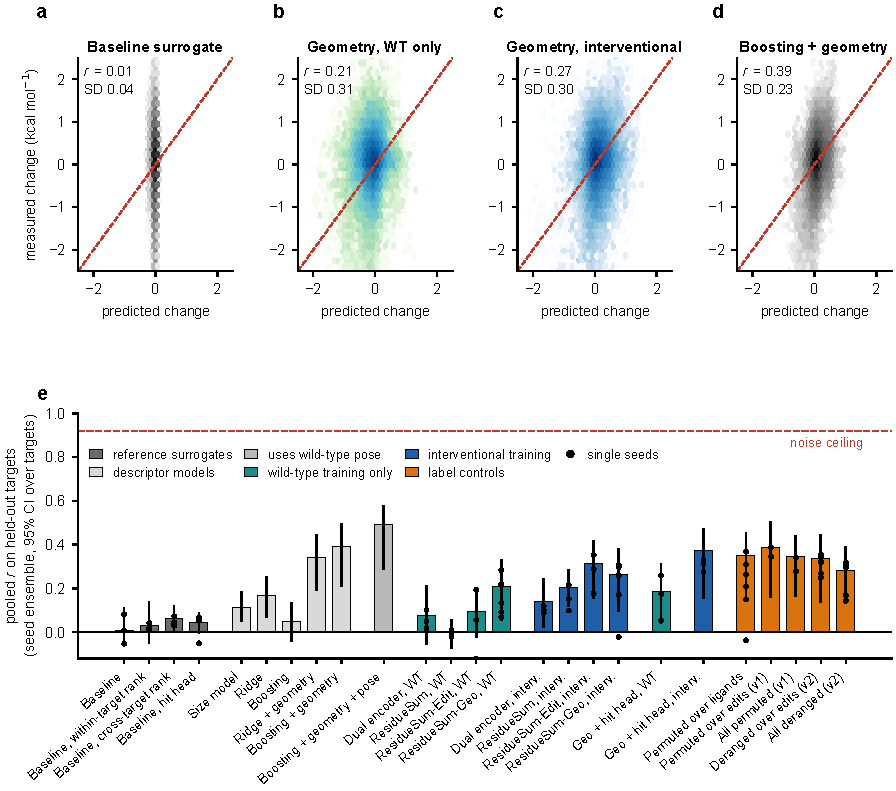
\includegraphics[width=\linewidth]{figures/fig3_main}
\caption{Prediction of measured score changes on the 19 held-out targets. (a--d) Predicted against measured change for the ensemble of the baseline surrogates, the geometry network trained on wild-type scores, the geometry network trained on measured changes and a boosting model on descriptors (hexagonal bins, logarithmic color, dashed line = identity), with the correlation $r$ and the standard deviation of the predicted change in \kcal{}. (e) Pooled correlation of every condition for the seed ensemble (bars, 95\% interval over targets) and for single seeds (dots). The dashed line marks the noise ceiling set by the wild-type replicates. v1 is the first implementation of a permutation control and v2 its correction.}
\label{fig:main}
\end{figure}

\begin{figure}[!ht]
\centering
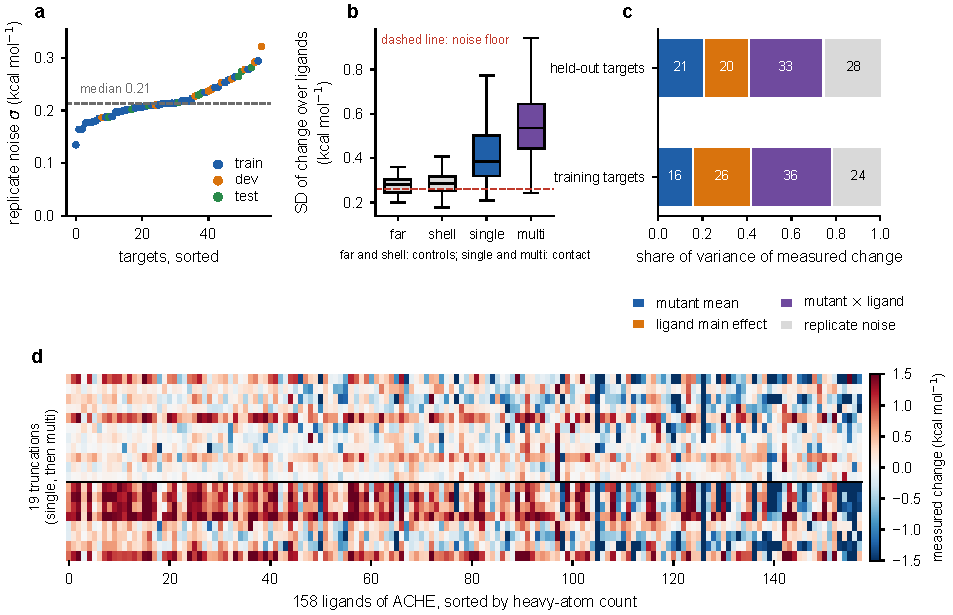
\includegraphics[width=\linewidth]{figures/fig2_response}
\caption{Response of the docking engine to receptor truncations. (a) Replicate noise of the wild-type score for each target. (b) Standard deviation over ligands of the measured change for shell and far controls, single contact truncations and multi-residue truncations; the dashed line marks the median noise of a change (\dsigmaMed{}~\kcal{}). (c) Share of the variance of measured changes held by the mean change of an edit, a ligand main effect, the edit-by-ligand interaction and replicate noise. (d) Measured changes for one held-out target (acetylcholinesterase): rows are truncations (single above the line, multi-residue below), columns are ligands ordered by heavy-atom count.}
\label{fig:response}
\end{figure}

The measured changes have a regular structure (Figure~\ref{fig:response}c,d). Replicate noise accounts for \shareNoise{}\% of their variance, the mean change of an edit for \shareMutant{}\%, a ligand main effect shared by all edits of a target for \shareLigand{}\% and the edit-by-ligand interaction for \shareInter{}\%. The ligand main effect follows a size law: in \nNegSlope{} of \nSlopeTargets{} targets, larger ligands gain more from a truncation than smaller ones. Figure~\ref{fig:response}d shows the pattern for acetylcholinesterase, where multi-residue truncations worsen the scores of small ligands and improve those of large ligands. The slope of this size dependence ranges from \slopeMin{} to \slopeMax{}~\kcal{} per heavy atom and is steeper in buried pockets ($r$ = \rBuried{} with the buried fraction of free space and \rAtomsTen{} with the number of receptor atoms within 10~\AA{} of the box center). Part of the interaction term follows the pose. For single contact truncations, the mean absolute change of a ligand rises from \contactNone{}~\kcal{} when no atom of its wild-type pose lies within 4.5~\AA{} of the removed side chain to \contactMany{}~\kcal{} when six or more atoms do, a trend present in \nContactTargets{} of \nContactOf{} targets, and the number of contacts correlates with the size of the change at $r$ = \rPoseContact{}. Controls without contact change by \controlNoContact{}~\kcal{}.

\subsection{Baseline surrogates do not respond to pocket edits}

We asked the baseline surrogates to predict the same changes for the \nHeldTargets{} held-out targets. Each model received the graph of the edited pocket, and its predicted change is the score for the edited pocket minus the score for the wild-type pocket. The three seed ensembles of the baselines respond with standard deviations of \sdPredRefMin{} to \sdPredRefMax{}~\kcal{} and the nine single checkpoints with \sdCkptMin{} to \sdCkptMax{}~\kcal{}, which is \ratioSdRefMin{} to \ratioSdRefMax{} times (single checkpoints \ratioCkptMin{} to \ratioCkptMax{} times) smaller than the \sdTrue{}~\kcal{} of the measured changes (Figure~\ref{fig:main}a). The correlation with the measured changes over all contact edits is \rRefSeedMin{} to \rRefSeedMax{} for single seeds. The seed ensembles reach \rEnsCZero{} (95\% interval \rLoCZero{} to \rHiCZero{}), \rEnsCOne{} (\rLoCOne{} to \rHiCOne{}) and \rEnsCTwo{} (\rLoCTwo{} to \rHiCTwo{}) for the plain, the within-target ranking and the cross-target ranking objective, and they separate contact edits from shell and far controls with AUCs of \aucRefMin{} to \aucRefMax{}. The hit-probability head of the baselines, which ranked ligands in the preceding analysis, gives the same picture with seed ensembles of \rEnsCZeroL{}, \rEnsCOneL{} and \rEnsCTwoL{} for its minus logit (Table~\ref{tab:main}).

\siinputpatched{table2}{Table S7}{Table~\ref{tab:si_levels}}

\subsection{Pocket geometry gives a surrogate its first response to edits}

The residue-sum network without geometry is as blind as the baselines when it is trained on wild-type scores only (pooled $r$ = \rEnsRsWt{}, 95\% interval \rLoRsWt{} to \rHiRsWt{}). Ten geometric descriptors of the pocket in its global term change this. The geometry network trained on wild-type scores alone has never seen an edited receptor, and it predicts the measured changes with $r$ = \rEnsRsgWt{} (\rLoRsgWt{} to \rHiRsgWt{}; \nSeedRsgWt{} seeds). The wild-type data already contain a relation that can produce this response: the score of a ligand depends on the size of the cavity, the descriptors expose that size to the network, and removing a side chain moves the prediction along the learned relation.

The response does not come from the residue graph. Removing the residue terms at inference, so that the score keeps only the ligand term and the global descriptor term, leaves the pooled correlation of the seed ensemble at \ablNoResRsgWt{} for the geometry networks trained on wild-type scores (full model \ablFullRsgWt{}), \ablNoResRsgInt{} for the geometry networks trained on measured changes (\ablFullRsgInt{}) and \ablNoResRsghInt{} for the networks with a hit head (\ablFullRsghInt{}). The predicted change of these networks is a function of the ligand embedding and the ten descriptors, and the residue graph adds no measurable response.

Interventional training raises the pooled correlation for the geometry-free residue-sum network, which goes from \rEnsRsWt{} to \rEnsRsInt{} (difference \diffRsIntMinusRsWt{}, 95\% interval \diffLoRsIntMinusRsWt{} to \diffHiRsIntMinusRsWt{}), and for the network that also receives an edit record, which goes from \rEnsRseWt{} to \rEnsRseInt{} (difference \diffRseIntMinusRseWt{}, interval \diffLoRseIntMinusRseWt{} to \diffHiRseIntMinusRseWt{}) (Figure~\ref{fig:main}e, Table~\ref{tab:main}); no label-shuffled control was trained for the geometry-free architecture. The increase is unresolved for the geometry network (\rEnsRsgWt{} to \rEnsRsgInt{}, difference \diffRsgIntMinusRsgWt{}, interval \diffLoRsgIntMinusRsgWt{} to \diffHiRsgIntMinusRsgWt{}) and for the dual encoder (\rEnsBfiveWt{} to \rEnsBfiveInt{}). The measured changes thus give a geometry-free network a response that a geometry network obtains from wild-type data, and they add a smaller increment on top of geometry. The edit-record network has the highest neural correlation (\rEnsRseInt{}), and the geometry network selected by the registered rule reaches \rEnsRsgInt{}; the two differ by \diffRsgIntMinusRseInt{} (\diffLoRsgIntMinusRseInt{} to \diffHiRsgIntMinusRseInt{}). All networks stay far below the noise ceiling of \ceilingR{} that follows from the wild-type replicates.

The hit head leaves this response intact (Table~\ref{tab:si_hyper} and Table~\ref{tab:main}). The network with a hit head, trained with three seeds and without label controls, reaches $r$ = \rEnsRsghWt{} without edited receptors and \rEnsRsghInt{} (\rLoRsghInt{} to \rHiRsghInt{}) with interventional training, for the seed ensemble (single seeds \rSeedMinRsghInt{} to \rSeedMaxRsghInt{}). This is \diffRsghIntMinusRsgInt{} above the six-seed registered geometry network (interval \diffLoRsghIntMinusRsgInt{} to \diffHiRsghIntMinusRsgInt{}) and \diffRsghIntMinusRsghWt{} above its wild-type-only version (\diffLoRsghIntMinusRsghWt{} to \diffHiRsghIntMinusRsghWt{}). It differs from the boosting model with pocket geometry by \diffRsghIntMinusGbmGeo{} (\diffLoRsghIntMinusGbmGeo{} to \diffHiRsghIntMinusGbmGeo{}).

\subsection{Label controls and descriptor models show what the response contains}

The analysis plan named two conditions for a claim that training on measured changes teaches a network to read the pocket: a pooled $r$ above the descriptor models and above both controls with permuted labels, with intervals over targets that exclude the control values. Neither condition holds. The geometry network trained on measured changes reaches $r$ = \rEnsRsgInt{} (\rLoRsgInt{} to \rHiRsgInt{}) for the seed ensemble. A boosting model on ligand descriptors, edit descriptors and pocket geometry reaches \rEnsGbmGeo{} (\rLoGbmGeo{} to \rHiGbmGeo{}), which exceeds the network by \diffGbmGeoMinusRsgInt{} (\diffLoGbmGeoMinusRsgInt{} to \diffHiGbmGeoMinusRsgInt{}), and the same model without the pocket descriptors reaches \rEnsGbmDesc{}. Networks trained on labels that were permuted over ligands, over edits or over all pairs give \rEnsRsgShl{}, \rEnsRsgShm{} and \rEnsRsgSha{}. The first implementation of the last two drew uniform permutations, which leave the row of an edit in place with probability one in six, so that these controls kept a fraction of the edit-specific signal. We corrected this after the held-out results were known and trained derangements instead, which give \rEnsRsgShmTwo{} and \rEnsRsgShaTwo{}. The corrected controls do not fall below the networks trained on measured labels: the difference in $r$ (measured labels minus control) is \diffRsgIntMinusRsgShmTwo{} (interval \diffLoRsgIntMinusRsgShmTwo{} to \diffHiRsgIntMinusRsgShmTwo{}) for the derangement over edits and \diffRsgIntMinusRsgShaTwo{} (\diffLoRsgIntMinusRsgShaTwo{} to \diffHiRsgIntMinusRsgShaTwo{}) for the derangement of all labels.

Pooled $r$ mixes differences between targets, between the edits of one target and between ligands. Separating these levels shows where the response sits (Figure~\ref{fig:levels}a--c). Within a target, the geometry network trained on measured changes reaches $r$ = \lvTargetRsgInt{}, the corrected controls \lvTargetRsgShmTwo{} and \lvTargetRsgShaTwo{}, and the boosting model with geometry \lvTargetGbmGeo{}. The edit means of a target, which rank the truncations by how strongly they move the scores, are predicted with \lvEditRsgInt{} by the geometry network, \lvEditRsgShmTwo{} and \lvEditRsgShaTwo{} by the corrected controls, \lvEditRsgWt{} by the geometry network without edited receptors and \lvEditGbmGeo{} by the boosting model. The ligand-specific part, the variation between ligands for one edit, stays at \lvLigRsgInt{} for the geometry network and \lvLigGbmGeo{} for the boosting model, and it reaches \lvLigGbmPoseGeo{} when the boosting model also receives the number of ligand atoms that touch the removed side chain in the wild-type pose. The ceiling for this level is \ceilLig{}. The ligand-specific part combines the ligand main effect and the edit-by-ligand interaction, and every model leaves most of it unexplained (Table~\ref{tab:si_levels}).

\begin{figure}[!ht]
\centering
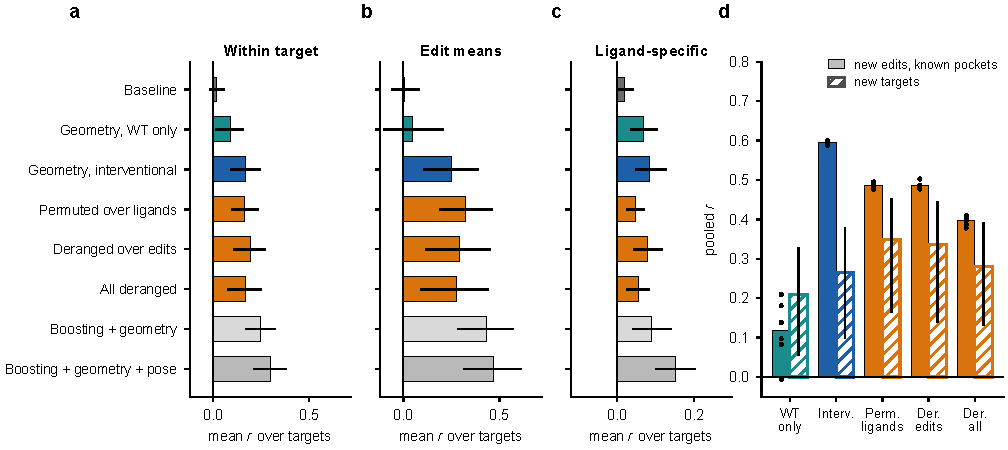
\includegraphics[width=\linewidth]{figures/fig4_levels}
\caption{Where the response comes from. Mean over the 19 held-out targets of (a) the correlation within a target over all contact pairs, (b) the correlation of the edit means within a target and (c) the ligand-specific correlation within an edit, with 95\% intervals over targets. (d) Pooled correlation for new edits of the training targets (15\% of their truncated receptors, withheld from training; solid bars with seeds as dots) and for new targets (hatched bars, seed ensemble with 95\% interval).}
\label{fig:levels}
\end{figure}

Measured labels make a difference where the network has seen the pocket or its relatives (Figure~\ref{fig:levels}d). For the 15\% of truncated receptors of each training target that were withheld from training (\shareMultiTrain{}\% of the contact edits among them are multi-residue truncations), the geometry network trained on measured changes reaches $r$ = \knownRRsgInt{} (SD over \nSeedRsgInt{} seeds \knownRSdRsgInt{}). Networks trained on deranged labels reach \knownRRsgShmTwo{} and \knownRRsgShaTwo{}, the control that permutes labels over ligands \knownRRsgShl{}, and the geometry network without edited receptors \knownRRsgWt{}. Measured labels thus carry edit-specific knowledge worth 0.1 to 0.2 in $r$ for a pocket the network has seen, and the controls show that the remaining 0.4 to 0.5 comes from what any label set of a target contains, namely the scale of its responses and its ligand main effect. For a target of an unseen family the edit-specific knowledge brings no measurable gain in any of the three levels (Figure~\ref{fig:main}e and Figures~\ref{fig:levels}a--c).

\subsection{The response to edits grows with the number of edits and transfers within a family}

The response to edits in new targets rises with the number of edits per training target (Figure~\ref{fig:scale}b). Pooled $r$ on the held-out targets is \scaleRMkTwo{} with 2 edits kept per training target, \scaleRMkEight{} with 8, \scaleRMkTwelve{} with 12 and \scaleRFull{} with all edits (on average \editsAllMean{}), and the 15\% withhold leaves \editsLeftTwo{}, \editsLeftEight{}, \editsLeftTwelve{} and \editsLeftFull{} edits for training. It also rises with the number of training targets, from \scaleRNtFour{} with 4 targets through \scaleRNtSixteen{} with 16 to \scaleRNtTwentyfour{} with 24 and \scaleRFull{} with all 38 (Figure~\ref{fig:scale}a). Each setting was trained with two seeds that differ by up to 0.29, so that the trends carry information and single points do not. The scaling runs have no label controls, and the network trained on wild-type scores alone reaches \rEnsRsgWt{} on the same targets, so the curves show how many edits and targets interventional training needs to reach that level.

\begin{figure}[!ht]
\centering
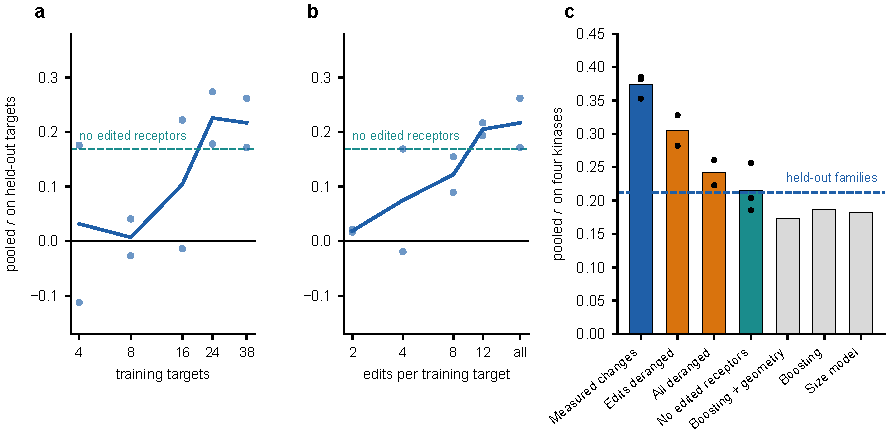
\includegraphics[width=\linewidth]{figures/fig5_scale}
\caption{The response to edits grows with the number of edits and transfers within a family. The scaling runs (a, b) have no label controls. Pooled correlation on the 19 held-out targets after training with (a) fewer training targets and (b) fewer edits per training target (dots: two seeds; line: mean; dashed line: geometry network without edited receptors, mean of six seeds). (c) Pooled correlation on four kinases withheld from training (ABL1, EGFR, SRC, JAK2) for the geometry network trained on measured changes, its controls and descriptor models fitted on the same training targets (dots: seeds; dashed line: the same network on the 19 held-out targets of other families).}
\label{fig:scale}
\end{figure}

Four kinases (ABL1, EGFR, SRC and JAK2) were withheld together with all their edits and the network was trained on the other 34 training targets, which include 17 further kinases (Figure~\ref{fig:scale}c). The geometry network trained on measured changes predicts the withheld kinases with $r$ = \kinRRsgInt{} (\kinNRsgInt{} seeds), against \kinRRsgWt{} for the network without edited receptors, \kinRRsgShmTwo{} and \kinRRsgShaTwo{} for deranged labels (\kinNRsgShmTwo{} seeds each) and \kinRGbmGeo{} for the boosting model with geometry. The edit means of the withheld kinases are predicted with \kinEditRsgInt{} by the network trained on measured changes and with \kinEditRsgShmTwo{} and \kinEditRsgShaTwo{} by the controls. The result covers four targets and has no interval over targets. The network trained on measured changes exceeds the controls with deranged labels by \kinGapRsgShmTwo{} and \kinGapRsgShaTwo{} in pooled $r$.

\subsection{The cached state evaluates edited pockets in a virtual alanine scan}

The same state evaluates an edited pocket by re-encoding it. We used this to truncate every residue with a side chain within 14~\AA{} of the box center of one held-out target, which was fixed before the scan as the target with the median per-target correlation (DHFR, \scanEdits{} residues), and to predict the change of the score of all \scanLig{} ligands (Figure~\ref{fig:scan}). The \scanModels{} seeds evaluated \scanPairs{} million ligand-edit pairs in \scanAllSec{} s, of which \scanQuerySec{} s were queries and the rest featurization and the construction of the edited graphs, against \dockDays{} GPU-days of docking, about \speedup{} times the time of the scan.

\begin{figure}[!ht]
\centering
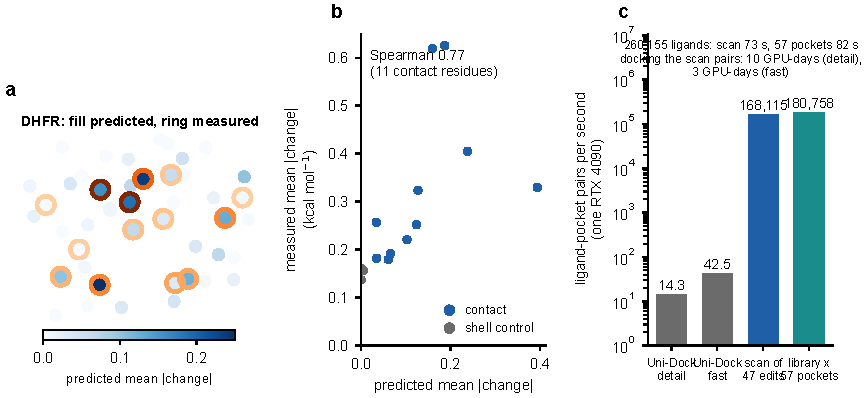
\includegraphics[width=\linewidth]{figures/fig7_scan}
\caption{Throughput of the cached pocket state and virtual alanine scan of a held-out target (DHFR, the target with the median per-target correlation). (a) C$\alpha$ positions of the 47 scanned residues projected on the plane of largest spread, filled by the predicted mean absolute change of the truncation over 260,155 ligands (three-seed ensemble of the geometry network) and ringed by the measured mean absolute change over 160 ligands for the 14 docked residues. (b) Predicted against measured mean absolute change of the docked residues. (c) Ligand-pocket pairs per second of GPU docking (Uni-Dock, detail and fast mode at the batch size with the highest rate), of the virtual scan of 47 edits and of the screen of the library against 57 wild-type pockets, on one RTX 4090 (ensemble of the three registered geometry networks without hit head, including ligand featurization and, for the scan, the construction of the edited graphs).}
\label{fig:scan}
\end{figure}

The predicted map agrees with the measured one in magnitude and differs in sign. Across the \scanNContact{} contact residues of DHFR with measured changes, the predicted mean absolute change has a Spearman correlation of \scanSpearmanAbs{} with the measured one (\scanSpearmanAbsAll{} with the three shell controls included), while the predicted mean signed change has $r$ = \scanRSigned{} with the measured one. Over all held-out targets the ranking of single contact truncations by predicted mean absolute change has a mean Spearman correlation of \hotRsgInt{} with the measured ranking, against \hotDist{} for the distance of the residue to the box center alone. The scan ranks the single contact truncations of a target below the distance of the residue to the box center (mean Spearman correlation \hotRsgInt{} against \hotDist{}), and its ligand-specific predictions correlate with the measured ones at \lvLigRsgInt{} against a ceiling of \ceilLig{} (Figure~\ref{fig:levels}c).


\section{Extended results of wild-type screening}

\subsection{Regression-trained networks and cross-target ordering}

The regression-trained networks rank less well than the hit-head networks (Table~\ref{tab:wt}, Figure~\ref{fig:wt}). Recall in this subsection is the top-1\% recall within the best 10\% of the ranking. The geometry network recovers \wtRTestRsgWt{} with wild-type training and \wtRTestRsgInt{} with interventional training, the residue-sum network without geometry \wtRTestRsWt{}, the network with an edit record \wtRTestRseWt{} and the dual encoder trained with the present recipe \wtRTestBfiveWt{}. The geometry network exceeds the geometry-free network by \wtdTestRsgWtMinusRsWt{} (interval \wtdLoTestRsgWtMinusRsWt{} to \wtdHiTestRsgWtMinusRsWt{}) on the test targets and by \wtdDevRsgWtMinusRsWt{} (\wtdLoDevRsgWtMinusRsWt{} to \wtdHiDevRsgWtMinusRsWt{}) on the development targets. Interventional training lifts the geometry-free network (\wtRTestRsWt{} to \wtRTestRsInt{}, interval of the difference \wtdLoTestRsIntMinusRsWt{} to \wtdHiTestRsIntMinusRsWt{}) and leaves the geometry network at the level of wild-type training (\wtdTestRsgIntMinusRsgWt{}, interval \wtdLoTestRsgIntMinusRsgWt{} to \wtdHiTestRsgIntMinusRsgWt{}), so the test gain of the descriptors is not specific to them. The hit head adds \hndTestRsghWtMinusRsgWt{} and \hndTestRsghIntMinusRsgInt{} to the two geometry networks, with 34,627 additional parameters.

The reversal accuracy measures the ordering of ligand pairs whose order flips between two targets. The hit logit of the hit-head networks reproduces both orderings in \hnJDevRsghWt{} and \hnJDevRsghInt{} of the development quadruplets and \hnJTestRsghWt{} and \hnJTestRsghInt{} of the test quadruplets, and the baseline surrogates with the plain, the within-target ranking and the cross-target ranking objective reach \hitJDevCZero{}, \hitJDevCOne{} and \hitJDevCTwo{} on the development targets and \hitJTestCZero{}, \hitJTestCOne{} and \hitJTestCTwo{} on the test targets (the last objective at a recall of \hitRTestCTwo{}). A model that ranks ligands identically in every target scores zero, as the constant pocket does, and a random model scores 0.25. The score head of the hit-head networks reaches \hnScoreJDevRsghWt{} and \hnScoreJDevRsghInt{} on the development quadruplets, and the regression-trained geometry networks \wtJDevRsgWt{} (range over \wtNDevRsgWt{} seeds \wtJminDevRsgWt{} to \wtJmaxDevRsgWt{}) and \wtJDevRsgInt{} (\wtJminDevRsgInt{} to \wtJmaxDevRsgInt{}), against \wtJDevRsgShmTwo{} and \wtJDevRsgShaTwo{} for the controls with deranged labels. The test targets show a smaller effect: the geometry networks reproduce both orderings in \wtJTestRsgWt{} and \wtJTestRsgInt{} of the test quadruplets and the controls in \wtJTestRsgShmTwo{} and \wtJTestRsgShaTwo{}. A boosting model on ligand descriptors and the ten pocket descriptors reaches \wtJDevBoostGeo{} on the development quadruplets and a recall of \wtRDevBoostGeo{}, against \wtJDevBoostLig{} and \wtRDevBoostLig{} without the pocket descriptors and \wtJDevRsgInt{} for the geometry network trained on measured changes.

\begin{table}[t]
\caption{Wild-type screening and cross-target ordering. Top-1\% recall within the best 10\% of the ranking (macro average over targets; 95\% interval from bootstrapping targets) and reversal accuracy, the fraction of quadruplets of two ligands and two targets in which both opposite orderings are reproduced (mean over seeds with range). The baseline surrogates have two readouts. The hit-probability head ranked ligands in the preceding analysis (values taken from its result files), the regression head gives the predicted score that is used for the edits in this study. The development split holds 10 targets and 10{,}025 quadruplets, the test split 9 targets and 3{,}536 quadruplets. Recall of the hit-head networks is the mean of single networks, and the test labels were read once for all models except these networks and once more for them (a third read served the six networks of the comparison with joint networks, Table~\ref{tab:si_joint_runs}).}
\label{tab:wt}
\centering
\resizebox{\textwidth}{!}{%
\begin{tabular}{lrrrrrr}
\toprule
& \multicolumn{3}{c}{Development targets} & \multicolumn{3}{c}{Test targets} \\
\cmidrule(lr){2-4}\cmidrule(lr){5-7}
Model & Recall & 95\% interval & Reversal & Recall & 95\% interval & Reversal \\
\midrule
\multicolumn{7}{l}{\emph{Baseline surrogates, hit-probability head (readout of the preceding analysis)}} \\
\quad Plain objective & 0.75 & 0.55 to 0.89 & 0.01 (0.00 to 0.01) & 0.83 & 0.81 to 0.85 & 0.03 (0.02 to 0.03) \\
\quad Within-target ranking & 0.74 & 0.54 to 0.88 & 0.01 (0.01 to 0.02) & 0.78 & 0.76 to 0.81 & 0.04 (0.03 to 0.06) \\
\quad Cross-target ranking & 0.70 & 0.55 to 0.82 & 0.07 (0.02 to 0.16) & 0.63 & 0.59 to 0.67 & 0.12 (0.08 to 0.18) \\
\quad Plain objective, constant pocket & 0.74 & 0.56 to 0.88 & 0.00 (0.00 to 0.00) & 0.82 & 0.79 to 0.86 & 0.00 (0.00 to 0.00) \\
\quad Ligand-only fingerprint model (CatBoost) & 0.68 & 0.54 to 0.80 & 0.00 (0.00 to 0.00) & 0.70 & 0.67 to 0.74 & 0.00 (0.00 to 0.00) \\
\midrule
\multicolumn{7}{l}{\emph{Baseline surrogates, regression head (readout used for edits)}} \\
\quad Plain objective & 0.71 & 0.53 to 0.84 & 0.01 (0.00 to 0.01) & 0.73 & 0.71 to 0.76 & 0.06 (0.04 to 0.08) \\
\quad Within-target ranking & 0.72 & 0.55 to 0.85 & 0.02 (0.01 to 0.04) & 0.73 & 0.69 to 0.77 & 0.05 (0.04 to 0.07) \\
\quad Cross-target ranking & 0.69 & 0.54 to 0.82 & 0.02 (0.01 to 0.02) & 0.70 & 0.68 to 0.72 & 0.05 (0.04 to 0.07) \\
\quad Plain objective, constant pocket & 0.70 & 0.54 to 0.83 & 0.00 (0.00 to 0.00) & 0.74 & 0.70 to 0.79 & 0.00 (0.00 to 0.00) \\
\midrule
\multicolumn{7}{l}{\emph{Wild-type training only}} \\
\quad Dual encoder & 0.70 & 0.54 to 0.83 & 0.01 (0.01 to 0.02) & 0.72 & 0.69 to 0.75 & 0.03 (0.02 to 0.03) \\
\quad ResidueSum & 0.74 & 0.58 to 0.86 & 0.09 (0.06 to 0.13) & 0.67 & 0.61 to 0.72 & 0.07 (0.05 to 0.09) \\
\quad ResidueSum-Edit & 0.75 & 0.60 to 0.86 & 0.44 (0.34 to 0.57) & 0.81 & 0.76 to 0.86 & 0.11 (0.10 to 0.12) \\
\quad ResidueSum-Geo & 0.74 & 0.58 to 0.86 & 0.25 (0.10 to 0.37) & 0.80 & 0.76 to 0.84 & 0.12 (0.10 to 0.18) \\
\midrule
\multicolumn{7}{l}{\emph{Interventional training}} \\
\quad Dual encoder & 0.69 & 0.54 to 0.82 & 0.01 (0.00 to 0.01) & 0.73 & 0.69 to 0.77 & 0.02 (0.01 to 0.03) \\
\quad ResidueSum & 0.74 & 0.53 to 0.89 & 0.04 (0.03 to 0.04) & 0.79 & 0.75 to 0.83 & 0.04 (0.04 to 0.06) \\
\quad ResidueSum-Edit & 0.74 & 0.58 to 0.86 & 0.28 (0.26 to 0.31) & 0.80 & 0.74 to 0.84 & 0.10 (0.09 to 0.11) \\
\quad ResidueSum-Geo & 0.74 & 0.60 to 0.85 & 0.41 (0.37 to 0.49) & 0.78 & 0.73 to 0.82 & 0.10 (0.09 to 0.11) \\
\midrule
\multicolumn{7}{l}{\emph{Network with a hit head, hit-logit readout (addendum 7)}} \\
\quad ResidueSum-Geo with hit head, wild type only & 0.80 & 0.65 to 0.90 & 0.18 (0.07 to 0.32) & 0.83 & 0.80 to 0.86 & 0.04 (0.03 to 0.07) \\
\quad ResidueSum-Geo with hit head, measured changes & 0.78 & 0.62 to 0.90 & 0.08 (0.05 to 0.09) & 0.84 & 0.81 to 0.88 & 0.04 (0.03 to 0.04) \\
\midrule
\multicolumn{7}{l}{\emph{Label controls}} \\
\quad Labels permuted over ligands & 0.75 & 0.60 to 0.87 & 0.19 (0.08 to 0.28) & 0.81 & 0.77 to 0.85 & 0.08 (0.06 to 0.09) \\
\quad Labels deranged over edits (v2) & 0.75 & 0.61 to 0.85 & 0.27 (0.23 to 0.29) & 0.80 & 0.75 to 0.84 & 0.08 (0.07 to 0.09) \\
\quad All labels deranged (v2) & 0.75 & 0.60 to 0.86 & 0.15 (0.11 to 0.20) & 0.80 & 0.75 to 0.84 & 0.08 (0.07 to 0.09) \\
\bottomrule
\end{tabular}}
\end{table}


\begin{figure}[!ht]
\centering
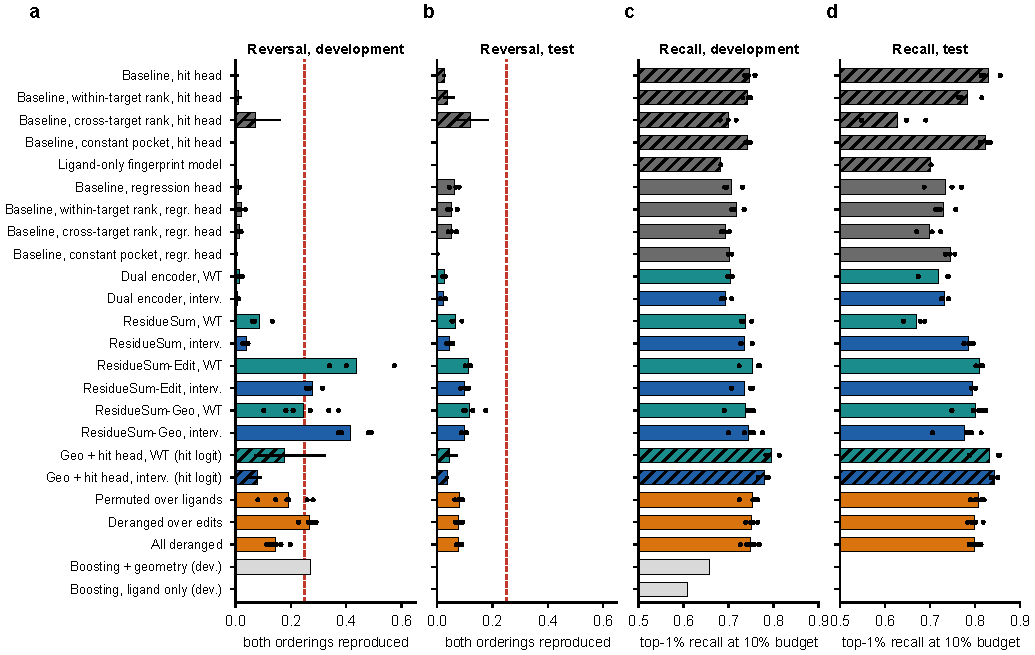
\includegraphics[width=\linewidth]{figures/fig6_wt}
\caption{Wild-type screening and cross-target ordering. Reversal accuracy (a, b) and top-1\% recall at a 10\% budget (c, d) on the development targets (a, c) and the test targets (b, d). Bars give the mean over seeds and dots single seeds. Hatched bars are the baseline surrogates read out with their hit-probability head, the readout of the preceding analysis (dots: seeds; line: range of the reversal accuracy over seeds); the regression head of the same checkpoints is shown below them. The dashed line marks random ordering in the reversal test. The descriptor models were evaluated on the development targets only. The recall axes start at 0.5.}
\label{fig:wt}
\end{figure}


\section{Registered analysis plan}

The plan below was hashed before the final interventional models were trained and before any of them was evaluated on the 19 held-out targets. A pilot of five short runs on six of the held-out targets preceded the hash (Disclosure below), so that the status line of the plan, which says that no interventional surrogate had been evaluated on the held-out targets, is incorrect. The hashed text cannot be edited, and this paragraph is its erratum. Addenda 1 to 4 were added before the evaluation of the final models. Addendum 5 was written after the registered runs had been evaluated and declares the correction of the permutation controls, the additional seeds and the post hoc analyses. The file and its hash ledger are part of the archive (\texttt{code/PREREG.md}, \texttt{code/prereg\_ledger.json}).

{\sloppy\subsection*{DockMut pre-registration (written before any held-out evaluation of interventional models)}

Status date: 2026-10-01. Re-docking data for held-out targets exist; no interventional surrogate has been evaluated on them. Family-level validation results exist only for the configuration choice described below.

\subsection*{Questions}

1. Do surrogates of the original study (real-pocket dual encoders, seeds 11/22/33 of C0, C1, C2) predict the docking-score change caused by truncating pocket residues on 19 held-out targets? 2. Does interventional training (measured changes of truncated receptors of the 38 training targets) give a surrogate that predicts these changes on unseen targets, and does it retain wild-type screening accuracy?

\subsection*{Data}

Held-out benchmark: 10 development and 9 test targets, 160 shared development ligands, up to 24 truncated receptors per target. Training: 38 training targets (DRD2 excluded), 256 ligands, up to 24 truncated receptors.

\subsection*{Primary outcome}

Pearson r between predicted and measured change over all (receptor, ligand) pairs of contact truncations (single and multi-residue) of the 19 held-out targets, with a bootstrap over targets for the 95\% interval. Secondary: mutant-level r, within-mutant r, regression gain, detection AUC of contact versus shell and far controls, and wild-type screening (top-1\% recall at 10\% budget, reversal accuracy on the frozen quads of the original study).

\subsection*{Conditions (three seeds 11, 22, 33 each, 20,000 updates, final checkpoint, no selection on held-out targets)}

rs\_wt, rs\_int, rs\_int\_shl (labels permuted across ligands within a receptor), rs\_int\_shm (labels permuted across receptors), rs\_const (one constant pocket), b5\_wt, b5\_int; and the same five ResidueSum conditions with geometry descriptors (rsg\_*). Descriptor baselines: size\_only, ridge\_descriptors, gbm\_descriptors.

\subsection*{Configuration choice (only validation on training targets is allowed to influence it)}

Validation = training on 30 training targets and evaluating on the 8 training targets of the families gpcr\_classA, cyp450 and serine\_protease\_S1 (all their truncated receptors). Candidates: rs\_int and rsg\_int with lambda in \{3, 10\}, rsg\_int with lambda 30, rsg\_int with learning rate $10^{-3}$, b5\_int with lambda 10. Rule: choose the candidate with the highest validation pooled r; differences below 0.02 are ties, broken toward ResidueSum without geometry. The chosen lambda, batch shape and learning rate are then fixed for all conditions.

\subsection*{Reporting}

All conditions, seeds and targets are reported whatever the outcome. The held-out benchmark is evaluated once per final model. Wild-type test labels (9 test targets) are read once, after the models are frozen, through the guarded label API, and the access is logged. Claims of pocket reading require, at the same time, a pooled r above the descriptor baselines and above both shuffled-label controls, with the bootstrap interval over targets excluding the control values.

\subsection*{Addendum 1 (before any held-out evaluation of an interventional model)}

Two validation candidates are added to the list above: rs\_int and rsg\_int with lambda 10 and family-balanced sampling of training targets (each protein family receives equal sampling mass). Predicted changes are clipped to the range of the training labels ($\pm$4 kcal/mol) in all evaluations. The batch shape for all candidates is six edited receptors on a shared set of 96 ligands per update. The selection rule is unchanged. Pilot runs used to debug the pipeline (eight training targets, six held-out targets, 3,000 to 6,000 updates) are disclosed in the Supporting Information and do not enter any reported number.

\subsection*{Addendum 2 (before any held-out evaluation of an interventional model)}

The control rs\_int\_shm (and rsg\_int\_shm) assigns each edit of a training step the measured change row of another edit of the same target evaluated on the same ligands. It destroys edit-specific information and keeps ligand main effects. An additional control rs\_int\_sha (and rsg\_int\_sha) permutes all measured changes of a step over (edit, ligand) pairs and keeps only their marginal distribution. The permutation across ligands within an edit (rs\_int\_shl) is unchanged.

\subsection*{Addendum 3 (secondary analyses, written before their execution)}

Secondary analyses of the selected configuration: (i) a scaling study with 4, 8, 16 and 24 random training targets (all edits) and with 2, 4, 8 and 12 edits per training target (all targets), two seeds each; (ii) a within-family transfer test in which four kinases (ABL1, EGFR, SRC, JAK2) are withheld from training and evaluated with all their edits, one seed; (iii) the seed ensemble of each condition; (iv) a virtual alanine scan of a held-out target with the full DOCKSTRING library of 260,155 ligands, reporting wall-clock time, and the agreement of the predicted mean change per residue with the measured mean change of the docked residues; (v) an independent check of measured changes with AutoDock Vina 1.1.2 on 32 ligands and four edits of three training targets. All are reported regardless of outcome.

\subsection*{Addendum 4 (written after the first validation round, before any held-out evaluation of an interventional model)}

First validation round (fold A: class A GPCRs, cytochromes P450 and S1 serine proteases withheld, 30 training targets), reported in the Supporting Information, gave validation pooled r between -0.12 and 0.17 for ten candidates. A gradient-boosting baseline that receives explicit edit descriptors and pocket geometry reached r 0.39 on the held-out targets, which shows that the edit record (removed atoms, distance, change of pocket geometry) carries transferable information. Because a single validation fold of eight targets has a large variance, the selection is repeated with two folds: fold A as above and fold B, in which the nine nuclear receptors are withheld (29 training targets). New candidates: rs\_wt and rsg\_wt (no intervention loss, reference), rsg\_int with lambda 1, and a ResidueSum-Edit architecture (rse) that adds an edit record (change of the ten geometry descriptors, removed atoms, edited residues, distance of the edit to the box center; zero for the wild type) to the global term. rse\_int is tried with lambda 3 and 10. All candidates with lambda $>$ 0 are trained on both folds (seed 11, 20,000 updates). Rule: choose the candidate with the highest mean validation pooled r over the two folds; differences below 0.02 are ties and are broken toward the simpler architecture (rs before rsg before rse), then toward the larger mean receptor-level r. The chosen configuration is fixed for all final conditions. The descriptor baselines are evaluated on both folds for reference.

\subsection*{Addendum 5 (written AFTER the held-out evaluation of all 36 registered final runs; everything below is post hoc)}

Registered outcome, stated before anything else: the pooled r of rsg\_int on the contact edits of the 19 held-out targets (seed ensemble 0.294, seed mean 0.247) is below that of the gradient-boosting baseline with pocket geometry (0.394) and below both shuffled-label controls as implemented (rsg\_int\_shm 0.387, rsg\_int\_sha 0.347 for the seed ensembles). The registered criterion for a claim of pocket reading is therefore not met.

Implementation error found while decomposing this result: the controls rsg\_int\_shm and rsg\_int\_sha used uniform random permutations. A uniform permutation of k = 6 edit rows leaves a given edit in place with probability 1/k (one fixed point on average per update), and a uniform permutation of all (edit, ligand) labels draws the label of an edit from its own row with probability 1/k. Both controls therefore carry the edit-specific signal at a dilution of 1/k, which contradicts the definition of Addendum 2 (the measured row of another edit). Corrected controls use a derangement of the edit rows (random cyclic shift of a random edit order by 1 to k-1 positions); rsg\_int\_sha2 additionally permutes the ligands independently within each row. They are run with three seeds under the registered settings and are reported next to the first implementation. The correction was made after the held-out results were known and it makes the control weaker, so it favors the hypothesis. The claim criterion is unchanged, and a claim of pocket reading requires that rsg\_int exceeds the descriptor baselines, the two first-implementation controls and the two corrected controls.

Post hoc analyses added after the registered outcomes were known (exploratory, labeled as such in the manuscript): (a) decomposition of faithfulness into target level, edit level within a target and ligand level within an edit (analysis\_levels.py); (b) a descriptor model that additionally receives contact counts from the wild-type pose; (c) a per-target analysis and a consensus of the neural ensemble with the descriptor model. No configuration is selected from these analyses.

\subsection*{Addendum 6 (written AFTER the first complete manuscript draft; post hoc)}

While reviewing the screening comparison we found that the baseline surrogates had been read out with their regression head, whereas the preceding analysis ranked ligands with their hit-probability head (a different output of the same dual encoder). The regression head gives a lower recall (0.72 against 0.83 on the nine test targets), so a comparison of the regression-trained networks of this study with the regression head of the baselines overstated the screening gain of the geometry descriptors. Corrections: (a) the hit-probability readout of the baselines is reported next to the regression readout, taken from the result files of the preceding analysis (no new label read; its development values were reproduced with dm\_baseline\_logit.py); (b) the response of the baselines to edits is repeated with the hit logit (dm\_baseline\_logit.py); (c) the text states that the geometry network reaches the screening recall of the hit-trained baselines within the resolution of nine targets and does not exceed it, and that the gain of the descriptors holds for networks trained with the same regression recipe. The registered outcomes and conditions are unchanged. Erratum: the hashed text gives 0.72 for the regression head on the nine test targets, and the value recomputed for Table~\ref{tab:wt} is \wtRTestCZero{}.

\subsection*{Addendum 7 (written AFTER addendum 6 and BEFORE any model of this extension was trained; post hoc relative to the registered plan)}

Motivation: the regression-trained geometry network matches but does not exceed the screening recall of the baselines that are trained on top-1\% hits (test recall 0.80 against 0.83). To test whether a Jev-like shared-state network with pocket geometry can reach the recall of hit-trained models while keeping its response to edits, ResidueSum-Geo receives a second readout, a hit logit computed from the same residue interaction features (modules lig\_off\_h, out\_h, glob\_h; the parameters of the registered score head start from identical values for the same seed).

Conditions (three seeds 11, 22, 33; 20,000 updates; final checkpoint; no selection): rsgh\_wt (no intervention loss) and rsgh\_int (intervention loss with lambda = 3). Loss = Huber on standardized scores + 1.0 x binary cross-entropy of the hit logit against the top-1\% hits of each training target (1st percentile of its training scores) + lambda x Huber on measured changes. Batch shape, optimizer and learning rate are those of the registered final runs. The weight of the hit loss is fixed to 1 before training and is not tuned.

Outcomes: (1) top-1\% recall at a 10\% budget with the hit logit on the 10 development targets and on the 9 test targets (frozen frames), and the reversal accuracy on the frozen quadruplets; (2) pooled r of the score head for the contact edits of the 19 held-out targets. Development metrics are computed on the pod, the test labels never leave the workstation and are read a SECOND time for these six models only (logged in runs/label\_access.log). All outcomes are reported whatever the result. A claim that the hit-head network reaches or exceeds the recall of the hit-trained baseline requires that the 95\% interval over targets of the paired difference to the plain-objective baseline (hit head) lies at or above zero.

Further measurements without labels on a rented RTX 4090 (the GPU class of the docking runs): the independence of the score of a ligand from the other candidates of a batch, the time to score the 260,155 ligands against all 57 wild-type pockets with the ligand embeddings computed once, and the time of the virtual alanine scan of DHFR. They replace the timings on the local RTX 4060 desktop of the first draft.

\subsection*{Addendum 8 (written AFTER the revision of the manuscript to the Jev-like framing and BEFORE any model of this comparison was trained; post hoc relative to the registered plan)}

Motivation: the manuscript claims that the Jev-like organization (pocket encoded once into a state, ligand embeddings that do not depend on the pocket, a cheap readout) gives surrogates that cost far less than joint networks for a library-against-many-pockets screen, at no loss of screening recall. Test: two joint surrogates are trained with the recipe of the baseline dual encoders (scripts/v3\_train\_joint.py, outputs in runs/v3): xattn, the PocketGate network in which ligand atoms attend to the residues of the pocket so that the ligand representation depends on the pocket, and pooled, PooledConcatNet, which concatenates pooled ligand and pocket vectors and reads them with a multilayer perceptron.

Conditions: seeds 11, 22 and 33 for each of the two networks. Settings are those of the baseline dual encoders of runs/v2 (AdamW, learning rate 3e-4, weight decay 1e-4, batches of 256 ligands of one training target, binary cross-entropy on the top-1\% hits plus 0.2 x Huber loss on standardized scores, at most 60,000 updates or 10 epochs, evaluation every 6,094 updates, patience of three evaluations, checkpoint = best macro Recall\_1\%@10\% on the cold development targets). No hyperparameter is tuned and nothing is changed after the first training run starts.

Outcomes: (1) top-1\% recall at the 1, 5, 10 and 20\% budgets on the 10 development targets and, after the checkpoints are frozen (sha256 in runs/v3/v3\_registry.json), on the 9 test targets with the frozen frames of the preceding analysis; the sealed test labels are read a THIRD time, once, only for these six models (logged in runs/label\_access.log); (2) the reversal accuracy on the frozen quadruplets; (3) the time to score the 260,155 ligands against the 57 wild-type pockets and against K pocket variants on one GPU for the joint networks (ligand atom states cached across pockets where the network allows it) and for the Jev-like networks. All outcomes are reported whatever the result.

Claim rule: the statement that the Jev-like dual encoders reach the screening recall of the joint networks requires that the lower limit of the 95\% interval over targets of the paired difference (dual encoder with its hit-probability head minus the joint network, test targets, 10\% budget) is at or above -0.03. If the joint networks exceed this margin, the manuscript reports the cost and the recall of both and states the trade-off.

\subsection*{Addendum 9 (written AFTER the review of the manuscript that followed addendum 8 and BEFORE any job of this extension was trained or timed; post hoc relative to the registered plan)}

Motivation: the review of the manuscript found three weaknesses of the comparison of addendum 8. (a) The recall at the 10\% budget of the nine test targets cannot separate networks that read the pocket from networks that do not: a network with one constant dummy pocket recovers 0.82 against 0.83, and every network, the cross-attention network included, outputs almost the same ligand ranking for every target. (b) The nine test targets are targets on which the shared ligand ranking works, and the cross-attention network was trained once with the recipe of the dual encoders. (c) The cost ratio of the joint network rests on a linear extrapolation of an unoptimized implementation measured on a desktop RTX 4060. This addendum registers two measurements on rented GPUs. Neither reads the sealed test labels.

Experiment E1 (cross-validation on 49 targets, scripts/v4\_cv\_train.py, dockmut/v4\_make\_folds.py, outputs in runs/v4): the 49 targets of the training and development roles are split into five folds of whole families (kinase; nuclear receptor; GPCR class A, CYP450 and MAOB; aspartyl protease, metalloprotease, serine protease S1, NOS1 and PARP1; PDE5A, PTGS2 and PTPN1), the assignment has the sha256 a9551800f8660b435c0636af04c771da34868893b49dcf2ab8e3b1803b6fba9f (data/splits/v4\_cv\_folds.json). For every fold the networks are trained on the targets outside the fold (training ligands of the preceding analysis, 40,000 per target) and evaluated on the held-out targets against the 10,000 development ligands, whose labels are open cells. Early stopping and the checkpoint rule use the macro Recall\_1\%@10\% over six targets drawn from the training targets of the fold against 10,000 ligands of the probability-calibration split (a deviation from the cold-development-target rule of the preceding analysis, because the folds consume the targets). Conditions: dual encoder, pooled-concatenation network and cross-attention network, each trained with the real pockets and with one constant synthetic pocket for every target (six conditions), recipe R0 (AdamW, learning rate 3e-4, weight decay 1e-4, batches of 256 ligands of one target, binary cross-entropy on the top-1\% hits plus 0.2 x Huber loss on standardized scores, at most 60,000 updates or 10 epochs, evaluation every 6,094 updates, patience of three evaluations), seed 11 first and seed 22 added if the first seed finishes within the budget of the rented time. A second recipe R1 (learning rate 1e-4, patience of eight evaluations, at most 150,000 updates or 30 epochs) is run for the dual encoder and the cross-attention network with the real pockets, to test whether the cross-attention network was undertrained. No hyperparameter is tuned and nothing is changed after the first job starts.

Outcomes of E1, all reported whatever the result: (1) top-1\% recall at the 1, 5, 10 and 20\% budgets per held-out target and as the macro mean over the 49 targets, with 95\% percentile intervals from 5,000 bootstrap resamples of the targets; (2) the pocket gain of each architecture, the paired difference between the network and its constant-pocket twin; (3) the selectivity, the correlation of the ligand-centered predictions with the ligand-centered docking scores within a fold, and the reversal accuracy on quadruplets drawn within each fold; (4) the same outcomes on the targets whose shared-ranking oracle recall (the recall of the ranking by the mean docking score over the training targets) is below 0.5.

Claim rules of E1: (a) the statement that the dual encoder reaches the screening recall of a joint network on 49 targets requires that the lower limit of the 95\% interval of the paired difference (dual encoder minus network, 10\% budget) is at or above -0.03, for the cross-attention network in recipes R0 and R1 and for the pooled network; (b) a network is said to read the pocket only if the lower limit of its pocket gain at the 10\% budget is above zero and its selectivity exceeds that of the constant-pocket twin (zero by construction); (c) otherwise the manuscript states that the network does not read the pocket under this recipe.

Experiment E2 (cost at the full scale, dockmut/v4\_fair\_timing.py): on one rented RTX 4090 the complete DOCKSTRING library of 260,155 ligands is screened from SMILES against 1, 5, 20 and 57 wild-type pockets, and against 1,000 pockets obtained by cycling the 57 pockets, with the dual encoder (matrix product), the pooled network (decomposed first layer) and the cross-attention network in its original padded float32 form, in a ragged float32 form and in a ragged float16 form, after a check that every optimized scorer reproduces the reference module (rank correlation of at least 0.9999 in float32 and 0.999 in float16). The stages (featurization, embedding, pocket states, scoring) and the end-to-end time are reported as measured, and the ratio of the cross-attention network to the dual encoder replaces the extrapolated ratio of addendum 8 in the manuscript, whatever its value.

\subsection*{Addendum 10 (written AFTER the experiments of addendum 9 and BEFORE the known-pocket evaluation was computed; post hoc relative to the registered plan)}

Scope decision: the manuscript is restricted to the pockets of the training data (known pockets), the setting in which the surrogates are used as multi-pocket screening engines after a docked training sample exists for each pocket. The cross-validation on held-out target families of addendum 9 (runs/v4, dockmut/eval/v4\_cv\_summary.json) was completed and is kept in the data archive; it is not part of the Results of the manuscript, which states the restriction to known pockets in the Discussion and lists addendum 9 in the Supporting Information.

Experiment E3 (known-pocket evaluation, dockmut/v5\_known\_pockets\_eval.py, outputs in runs/v5): the existing checkpoints of the dual encoder (runs/v1 and runs/v2, seeds 11, 22 and 33), the dual encoder with one constant synthetic pocket (three seeds), the pooled-concatenation network and the cross-attention network (runs/v3, three seeds each) are evaluated on the 39 training targets against the 10,000 development ligands (labels of the open cell train x dev; no sealed label is read). The development ligands were never training ligands of these networks; the checkpoint rule of these networks used the cold development targets only. Outcomes, all reported whatever the result: top-1\% recall at the 1, 5, 10 and 20\% budgets per target and as the macro mean over the 39 targets (mean over seeds per target), with 95\% percentile intervals from 5,000 bootstrap resamples of the targets, and paired differences between networks; the model times of addendum 9 (experiment E2) give the cost side. The manuscript states the recall of the shared-state networks as a fraction of the recall of the cross-attention network with its interval.

\subsection*{Addendum 11 (written AFTER the outcomes of experiment E3 of addendum 10 were known and BEFORE the cross-fitted known-pocket evaluation was computed; post hoc)}

Reason: the checkpoint rule of the networks of experiment E3 (macro recall on the cold development targets) selects checkpoints for new targets, and it can select early checkpoints that do not suit the pockets of the training data. E3 gave top-1\% recall at the 10\% budget of 0.860 (dual encoder), 0.849 (pooled network), 0.847 (cross-attention network) and 0.833 (constant pocket) on the 39 training pockets. The networks of the cross-validation runs of addendum 9 choose their checkpoint on seen targets (six validation targets of the training targets of the fold against 10,000 calibration ligands) and therefore suit the known-pocket setting. Experiment E4 (dockmut/v5\_known\_cv\_eval.py, outputs in runs/v5): every network of a fold (conditions dual, pooled and cross-attention with the real pockets and with the constant pocket, recipe R0, and the recipe R1 for the dual encoder and the cross-attention network, seed 11) is evaluated on the pockets of its training targets against the 10,000 development ligands (open labels; neither training nor checkpoint choice used them). The recall of a pocket is the mean over the folds in which the pocket is a training target (four of five); summaries are macro means over the 49 pockets with 95\% bootstrap intervals and paired differences, as in E3. Both E3 and E4 are reported whatever the result.
}

\begin{table}[h]
\caption{Hash ledger of the analysis plan. Each entry is the SHA-256 of \texttt{PREREG.md} at the time of writing, with the UTC time and the status of the plan.}
\label{tab:si_ledger}
\small
\begin{tabular}{llp{0.4\linewidth}}
\toprule
UTC time & SHA-256 (first 16 characters) & Status \\
\midrule
2026-09-30 19:30:14 & \texttt{73b1b19de9149032} & before any held-out evaluation of interventional models \\
2026-09-30 19:52:32 & \texttt{fa6d5a13017ffaf1} & addendum 1: family-balanced candidates, clipping \\
2026-09-30 19:57:29 & \texttt{1c290539b171b3b9} & addendum 2: definition of shuffled-label controls \\
2026-09-30 20:07:10 & \texttt{3321ebcacf1c330e} & addendum 3: secondary analyses \\
2026-09-30 20:50:42 & \texttt{784f64788e89b299} & addendum 4: two-fold validation, rse architecture \\
2026-09-30 21:58:36 & \texttt{196154fdbc62f984} & addendum 5: written after the held-out evaluation of the 36 registered final runs; controls corrected (derangement), post hoc analyses declared \\
2026-10-01 00:37:41 & \texttt{e43ddcc963d8d64b} & addendum 6: written after the first complete draft; baseline hit-probability readout added, screening comparison restated \\
2026-10-01 23:10:37 & \texttt{a475b8ae08597371} & addendum 7: hit-head extension and RTX 4090 throughput measurements, written before training \\
2026-10-08 04:52:36 & \texttt{fe844b5b28a1e5c4} & addendum 8: joint (cross-attention and pooled) surrogates trained with the baseline recipe, written before training \\
2026-10-08 15:43:10 & \texttt{b9287ae6713ba10e} & addendum 9: 49-target cross-validation with constant-pocket controls and full-scale timing, written before any job \\
2026-10-09 13:15:41 & \texttt{9aac3ced2790d242} & addendum 10: manuscript restricted to known pockets; known-pocket evaluation of the existing checkpoints, written before it was computed \\
2026-10-09 13:27:43 & \texttt{73b80ead375ecbb1} & addendum 11: cross-fitted known-pocket evaluation of the cross-validation networks, written after E3 and before E4 was computed \\
\bottomrule
\end{tabular}
\end{table}


\section{Disclosure of deviations and exploratory work}

Before the registered runs, a pilot on three targets (ABL1, MAOB, PTGS2) and 96 ligands compared docking search modes of Uni-Dock with the DOCKSTRING scores and with AutoDock Vina 1.1.2 and measured replicate noise. A dry run of the training pipeline used eight training targets, six held-out targets and between 3,000 and 6,000 updates, and a second pilot compared four hyperparameter variants of the geometry-free network with interventional training on the same six held-out targets. Both were evaluated before the plan was hashed, and their outputs are in the archive (\texttt{eval/pilot}). The dry run exposed that dropout in the pocket encoder hides the small difference between a wild-type and an edited pocket, and dropout was removed from the pocket encoders for all reported models. The pilots informed the candidate list of the plan, and none of their results enters a reported number.

The configuration was chosen on two validation folds inside the training targets (Table~\ref{tab:si_val}). The first round, on fold A alone, gave validation correlations between $-0.12$ and 0.17 for nine interventional candidates and 0.19 for the reference without intervention. A boosting model with pocket geometry reached $r$ = 0.39 on the held-out targets at that point, which led to the second round with two folds and the ResidueSum-Edit architecture (addendum 4). The registered rule selected ResidueSum-Geo with $\lambda$ = 3. The hashed addendum 4 describes the second round, and ResidueSum-Edit was added after the descriptor model had been evaluated on the held-out targets.

After the held-out evaluation of the 36 registered final runs we found that the two controls that permute labels over edits had used uniform permutations, which return an edit to its own row with probability one in six. The corrected controls (derangements) and three further seeds for five conditions were trained afterwards (addendum 5). The levels of faithfulness, the pose-informed descriptor reference, the descriptor model for wild-type screening, the hot-spot ranking and the virtual scan were added after the registered outcomes were known. After the first complete draft we found that the baseline surrogates had been read out with their regression head in the screening comparison, whereas the preceding analysis ranked ligands with their hit-probability head, which recovers more top hits for the plain objective (\hitRTestCZero{} against \wtRTestCZero{} on the test targets). The hit-probability readout was added from the result files of the preceding analysis, the response of the baselines to edits was repeated with the hit logit (rows of Table~\ref{tab:main}), and the text was restated (addendum 6). Last, ResidueSum-Geo received a hit head (addendum 7, written before the six networks were trained), a second readout on the same residue features that is trained on the top-1\% hits with a weight of 1, with and without the loss on changes and with three seeds each. The rule registered for a claim that this network reaches the recall of the hit-trained baseline, a paired interval at or above zero, was not met, and the extension is reported as post hoc. The development split was inspected before the test split was opened in both rounds. The test labels were read once for the 69 models of the first round and a second time for the six hit-head networks (Table~\ref{tab:si_access}).

Several registered items changed. The final runs omit the registered conditions rs\_int\_shl, rs\_int\_shm, rs\_int\_sha and rs\_const (the label controls and the constant-pocket condition of the geometry-free network) and include rse\_wt, rse\_int and rsg\_int\_sha, which were not in the original list, so that the geometry-free network has no label-shuffled control. The constant-pocket geometry network responds to an edit by zero by construction and is not tabulated, and its wild-type screening evaluation restored the real pockets, so that its screening row is not reported. The registered secondary outcome regression gain is stored in the archive (\texttt{eval/summary\_all.json}) and not tabulated, and the consensus of the neural ensemble with the descriptor model named in addendum 5 was not run. The kinase test of addendum 3 was registered with one seed and was run with three seeds for the network trained on measured changes, three for the wild-type-only network and two for each deranged control. The descriptor model for wild-type screening and the hot-spot ranking are not part of a hashed addendum and are described in the extended methods and results sections of this Supporting Information. Addendum 7 states that the score-head parameters of the hit-head networks start from the registered values for the same seed. The training script seeds the generator after it builds the model, so that the seed argument does not control the initial weights, the statement does not hold, and the hit-head networks were initialized independently of the registered networks.

After the registered outcomes were known, the screening results were extended with analyses that were not part of a hashed addendum: the docking rate benchmark, the network throughput of the three families, the budget summary of the wild-type screening (\texttt{eval/wt\_budget\_summary.json}, a re-summary of existing per-target result files, with no new label read) and an ML-guided docking baseline on the development targets (development labels only, caller \texttt{ml\_guided\_dev}; \texttt{eval/ml\_guided\_dev.json}, not reported in the manuscript). They are post hoc, no model, configuration or readout was selected from them, and the sealed test labels were not read for them. The first run of the docking benchmark skipped the batches of 1{,}024 ligands because one of the 1{,}024 prepared ligands failed preparation. The batches of 1{,}000 and 4{,}000 ligands were run afterwards on the same pod, and every call of all runs is in the records. The joint networks and the cost model (addendum 8) were added after the registered outcomes and the revision of the framing; the plan for them was hashed before the first run, the sealed test labels were read a third time, once, for the six joint networks (Table \ref{tab:si_access}), and no setting was changed after the first run started.

\begin{table}[h]
\caption{Reads of the sealed test labels through the guarded label interface (local time, UTC+9). The first three rows are single-row reads by unit tests of the label guard before any model existed, the next two belong to the preceding analysis, the sixth to the 69 models of the first round, the seventh to the six hit-head networks (addendum 7) and the last to the six joint networks (addendum 8).}
\label{tab:si_access}
\small
\begin{tabular}{llll}
\toprule
Time & Caller & Cell & Rows \\
\midrule
2026-09-22 21:58 & \texttt{pytest} & \texttt{test\_test} & 1 \\
2026-09-22 22:07 & \texttt{pytest} & \texttt{test\_test} & 1 \\
2026-09-22 22:11 & \texttt{pytest} & \texttt{test\_test} & 1 \\
2026-09-23 23:45 & \texttt{v2\_final\_eval} & \texttt{test\_test} & 234{,}135 \\
2026-09-23 23:45 & \texttt{v2\_final\_eval} & \texttt{train\_test} & 1{,}014{,}585 \\
2026-10-01 07:49 & \texttt{dm\_wt\_eval\_test} & \texttt{test\_test} & 234{,}135 \\
2026-10-02 08:33 & \texttt{dm\_wt\_eval\_test} & \texttt{test\_test} & 234{,}135 \\
2026-10-08 18:25 & \texttt{v3\_test\_eval} & \texttt{test\_test} & 234{,}135 \\
\bottomrule
\end{tabular}
\end{table}


\section{Supporting tables}

{\footnotesize\setlength{\tabcolsep}{3pt}\begin{longtable}{llp{2.4cm}rrrrrrrr}
\caption{Per-target summary of DockMut-1. $\sigma$ is the replicate noise of the wild-type score, $n_\mathrm{stable}$ the ligands kept after the stability filter, the four shares are fractions of the variance of measured changes in percent, and $r_\mathrm{WT}$ and MAE compare the wild-type scores of the GPU engine with the DOCKSTRING table (training and development targets only).}
\label{tab:si_targets}\\
\toprule
Target & Role & Family & Edits & $n_\mathrm{stable}$ & $\sigma$ & Mean & Ligand & Inter. & Noise & $r_\mathrm{WT}$ \\
\midrule
\endfirsthead
Target & Role & Family & Edits & $n_\mathrm{stable}$ & $\sigma$ & Mean & Ligand & Inter. & Noise & $r_\mathrm{WT}$ \\
\midrule
\endhead
BACE1 & dev & aspartyl protease & 21 & 160 & 0.23 & 20 & 7 & 37 & 39 & 0.94 \\
REN & dev & aspartyl protease & 20 & 160 & 0.21 & 26 & 18 & 33 & 25 & 0.96 \\
MAOB & dev & maob & 24 & 138 & 0.32 & 27 & 25 & 43 & 7 & 0.47 \\
ADAM17 & dev & metalloprotease & 17 & 160 & 0.24 & 11 & 20 & 27 & 45 & 0.94 \\
MMP13 & dev & metalloprotease & 21 & 160 & 0.24 & 22 & 17 & 30 & 33 & 0.93 \\
NOS1 & dev & nos1 & 19 & 160 & 0.25 & 27 & 23 & 34 & 18 & 0.91 \\
PARP1 & dev & parp1 & 19 & 159 & 0.28 & 36 & 18 & 15 & 32 & 0.94 \\
PDE5A & dev & pde5a & 22 & 160 & 0.19 & 32 & 20 & 34 & 17 & 0.95 \\
PTGS2 & dev & ptgs2 & 24 & 158 & 0.29 & 23 & 29 & 40 & 11 & 0.89 \\
PTPN1 & dev & ptpn1 & 21 & 157 & 0.26 & 39 & 19 & 24 & 19 & 0.91 \\
ACHE & test & ache & 23 & 158 & 0.22 & 16 & 36 & 41 & 9 & -- \\
CA2 & test & ca2 & 23 & 160 & 0.21 & 15 & 16 & 45 & 27 & -- \\
CASP3 & test & casp3 & 18 & 160 & 0.27 & 10 & 12 & 16 & 63 & -- \\
DHFR & test & dhfr & 23 & 160 & 0.19 & 33 & 17 & 35 & 16 & -- \\
DPP4 & test & dpp4 & 22 & 160 & 0.28 & 28 & 16 & 21 & 36 & -- \\
GBA & test & gba & 24 & 160 & 0.20 & 16 & 20 & 43 & 24 & -- \\
HMGCR & test & hmgcr & 19 & 158 & 0.26 & 2 & 14 & 32 & 55 & -- \\
HSD11B1 & test & hsd11b1 & 22 & 160 & 0.23 & 11 & 40 & 36 & 15 & -- \\
HSP90AA1 & test & hsp90aa1 & 23 & 159 & 0.23 & 3 & 18 & 48 & 33 & -- \\
CYP2C9 & train & cyp450 & 23 & 254 & 0.18 & 7 & 23 & 43 & 29 & 0.96 \\
CYP3A4 & train & cyp450 & 20 & 254 & 0.21 & 25 & 18 & 26 & 33 & 0.96 \\
ADORA2A & train & gpcr classA & 23 & 256 & 0.19 & 29 & 23 & 33 & 18 & 0.93 \\
ADRB1 & train & gpcr classA & 24 & 255 & 0.21 & 8 & 26 & 41 & 27 & 0.93 \\
ADRB2 & train & gpcr classA & 24 & 255 & 0.20 & 20 & 24 & 39 & 19 & 0.95 \\
DRD3 & train & gpcr classA & 23 & 255 & 0.14 & 15 & 32 & 48 & 8 & 0.95 \\
ABL1 & train & kinase & 21 & 252 & 0.22 & 8 & 35 & 46 & 14 & 0.76 \\
AKT1 & train & kinase & 24 & 256 & 0.21 & 21 & 8 & 27 & 46 & 0.95 \\
AKT2 & train & kinase & 24 & 251 & 0.22 & 20 & 23 & 35 & 24 & 0.92 \\
CDK2 & train & kinase & 19 & 255 & 0.20 & 13 & 21 & 32 & 36 & 0.93 \\
CSF1R & train & kinase & 20 & 256 & 0.21 & 27 & 24 & 34 & 17 & 0.91 \\
EGFR & train & kinase & 21 & 256 & 0.19 & 15 & 32 & 32 & 23 & 0.93 \\
FGFR1 & train & kinase & 22 & 254 & 0.24 & 6 & 30 & 46 & 21 & 0.88 \\
IGF1R & train & kinase & 20 & 256 & 0.21 & 2 & 31 & 39 & 31 & 0.88 \\
JAK2 & train & kinase & 18 & 256 & 0.18 & 10 & 36 & 34 & 23 & 0.95 \\
KDR & train & kinase & 24 & 253 & 0.20 & 17 & 26 & 43 & 16 & 0.91 \\
KIT & train & kinase & 20 & 256 & 0.23 & 5 & 38 & 38 & 23 & 0.93 \\
LCK & train & kinase & 17 & 255 & 0.20 & 6 & 31 & 28 & 37 & 0.95 \\
MAP2K1 & train & kinase & 24 & 254 & 0.20 & 9 & 18 & 38 & 37 & 0.96 \\
MAPK1 & train & kinase & 23 & 256 & 0.20 & 23 & 30 & 35 & 14 & 0.91 \\
MAPK14 & train & kinase & 21 & 253 & 0.26 & 7 & 16 & 25 & 53 & 0.90 \\
MAPKAPK2 & train & kinase & 22 & 254 & 0.19 & 11 & 27 & 37 & 27 & 0.95 \\
MET & train & kinase & 21 & 252 & 0.24 & 4 & 24 & 43 & 32 & 0.88 \\
PLK1 & train & kinase & 18 & 254 & 0.21 & 44 & 19 & 23 & 16 & 0.91 \\
PTK2 & train & kinase & 18 & 254 & 0.16 & 11 & 38 & 37 & 17 & 0.84 \\
ROCK1 & train & kinase & 24 & 256 & 0.18 & 18 & 18 & 35 & 31 & 0.95 \\
SRC & train & kinase & 22 & 255 & 0.18 & 28 & 25 & 35 & 15 & 0.93 \\
AR & train & nuclear receptor & 24 & 243 & 0.29 & 20 & 25 & 45 & 13 & 0.73 \\
ESR1 & train & nuclear receptor & 23 & 255 & 0.21 & 40 & 18 & 33 & 11 & 0.90 \\
ESR2 & train & nuclear receptor & 24 & 254 & 0.16 & 29 & 20 & 45 & 8 & 0.82 \\
NR3C1 & train & nuclear receptor & 24 & 254 & 0.22 & 7 & 48 & 37 & 10 & 0.93 \\
PGR & train & nuclear receptor & 24 & 250 & 0.28 & 17 & 39 & 38 & 8 & 0.67 \\
PPARA & train & nuclear receptor & 20 & 255 & 0.22 & 8 & 24 & 41 & 29 & 0.91 \\
PPARD & train & nuclear receptor & 24 & 255 & 0.21 & 5 & 12 & 42 & 43 & 0.93 \\
PPARG & train & nuclear receptor & 22 & 254 & 0.21 & 7 & 25 & 42 & 27 & 0.90 \\
THRB & train & nuclear receptor & 24 & 253 & 0.21 & 4 & 49 & 42 & 8 & 0.87 \\
F10 & train & serine protease S1 & 19 & 253 & 0.26 & 16 & 24 & 29 & 33 & 0.90 \\
F2 & train & serine protease S1 & 20 & 253 & 0.25 & 31 & 14 & 22 & 35 & 0.91 \\
\bottomrule
\end{longtable}
}

{\footnotesize\setlength{\tabcolsep}{3pt}\begin{longtable}{llp{3.3cm}rrrrr}
\caption{Validation of candidate configurations. Fold A withholds class A GPCRs, cytochromes P450 and S1 serine proteases, fold B withholds the nuclear receptors. Pearson $r$ over contact edits of the withheld families, the correlation of edit means, the within-edit correlation, the SD of the predicted change in \kcal{}, and $r$ for edits that were withheld from training targets (new edits of known pockets).}
\label{tab:si_val}\\
\toprule
Fold & Model & Setting & $r$ & Edit mean $r$ & Within $r$ & Pred. SD & New edits $r$ \\
\midrule
\endfirsthead
Fold & Model & Setting & $r$ & Edit mean $r$ & Within $r$ & Pred. SD & New edits $r$ \\
\midrule
\endhead
A & Dual encoder & $\lambda$ = 10 & 0.10 & 0.14 & 0.06 & 0.17 & 0.43 \\
A & ResidueSum & $\lambda$ = 10 & 0.17 & 0.28 & 0.04 & 0.18 & 0.54 \\
A & ResidueSum & $\lambda$ = 10, family balance & $-$0.12 & $-$0.17 & $-$0.02 & 0.31 & 0.56 \\
A & ResidueSum & $\lambda$ = 3 & 0.17 & 0.23 & 0.05 & 0.27 & 0.52 \\
A & ResidueSum & no intervention & $-$0.07 & $-$0.09 & $-$0.04 & 0.07 & $-$0.02 \\
A & ResidueSum-Edit & $\lambda$ = 10 & 0.01 & 0.07 & 0.05 & 1.13 & 0.60 \\
A & ResidueSum-Edit & $\lambda$ = 3 & 0.14 & 0.08 & 0.08 & 0.86 & 0.60 \\
A & ResidueSum-Edit & no intervention & 0.11 & 0.12 & 0.06 & 1.58 & 0.25 \\
A & ResidueSum-Geo & $\lambda$ = 1 & $-$0.08 & $-$0.12 & 0.05 & 1.12 & 0.55 \\
A & ResidueSum-Geo & $\lambda$ = 10 & 0.11 & 0.07 & 0.05 & 0.93 & 0.60 \\
A & ResidueSum-Geo & $\lambda$ = 10, family balance & 0.14 & 0.15 & 0.04 & 1.38 & 0.64 \\
A & ResidueSum-Geo & $\lambda$ = 10, rate $10^{-3}$ & $-$0.01 & $-$0.16 & 0.06 & 0.85 & 0.63 \\
A & ResidueSum-Geo & $\lambda$ = 3 & 0.12 & 0.07 & 0.06 & 0.77 & 0.58 \\
A & ResidueSum-Geo & $\lambda$ = 30 & $-$0.09 & $-$0.14 & 0.04 & 1.08 & 0.59 \\
A & ResidueSum-Geo & no intervention & 0.19 & 0.29 & 0.06 & 1.11 & 0.28 \\
B & ResidueSum & $\lambda$ = 10 & 0.09 & 0.14 & 0.06 & 0.18 & 0.55 \\
B & ResidueSum & $\lambda$ = 3 & 0.07 & 0.00 & 0.07 & 0.21 & 0.50 \\
B & ResidueSum & no intervention & $-$0.01 & $-$0.05 & 0.00 & 0.02 & 0.13 \\
B & ResidueSum-Edit & $\lambda$ = 10 & 0.24 & 0.33 & 0.09 & 0.28 & 0.53 \\
B & ResidueSum-Edit & $\lambda$ = 3 & 0.07 & $-$0.05 & 0.10 & 0.28 & 0.51 \\
B & ResidueSum-Edit & no intervention & 0.15 & $-$0.06 & 0.13 & 0.28 & 0.17 \\
B & ResidueSum-Geo & $\lambda$ = 1 & 0.18 & 0.08 & 0.13 & 0.26 & 0.49 \\
B & ResidueSum-Geo & $\lambda$ = 10 & 0.06 & $-$0.14 & 0.10 & 0.33 & 0.52 \\
B & ResidueSum-Geo & $\lambda$ = 3 & 0.22 & 0.21 & 0.12 & 0.30 & 0.50 \\
B & ResidueSum-Geo & no intervention & 0.16 & 0.08 & 0.13 & 0.35 & 0.17 \\
\bottomrule
\end{longtable}
}

{\footnotesize\setlength{\tabcolsep}{3pt}\begin{longtable}{p{4.6cm}rrrr}
\caption{Three levels of faithfulness on the 19 held-out targets (mean over targets with 95\% interval from bootstrapping targets). Within-target $r$ is computed over all contact pairs of one target, edit-mean $r$ over the receptor means of its contact edits, and ligand-specific $r$ within a receptor after removing the receptor mean. SD is the standard deviation of the predicted change in \kcal{}.}
\label{tab:si_levels}\\
\toprule
Model & Within target & Edit means & Ligand-specific & SD \\
\midrule
\endfirsthead
Model & Within target & Edit means & Ligand-specific & SD \\
\midrule
\endhead
\multicolumn{5}{l}{\emph{Baseline surrogates, regression head}} \\
\quad Plain objective & 0.02 [$-$0.01, 0.06] & 0.01 [$-$0.06, 0.08] & 0.02 [0.00, 0.04] & 0.03 \\
\quad Within-target ranking & 0.04 [0.00, 0.08] & 0.10 [0.01, 0.20] & $-$0.01 [$-$0.04, 0.02] & 0.03 \\
\quad Cross-target ranking & 0.03 [$-$0.01, 0.07] & 0.09 [0.00, 0.18] & $-$0.01 [$-$0.04, 0.01] & 0.02 \\
\multicolumn{5}{l}{\emph{Baseline surrogates, hit-probability head}} \\
\quad Plain objective & 0.01 [$-$0.02, 0.04] & $-$0.05 [$-$0.13, 0.04] & 0.02 [0.00, 0.04] & 0.08 \\
\quad Within-target ranking & $-$0.02 [$-$0.06, 0.01] & $-$0.08 [$-$0.18, 0.01] & $-$0.01 [$-$0.04, 0.02] & 0.10 \\
\quad Cross-target ranking & $-$0.03 [$-$0.06, 0.00] & $-$0.11 [$-$0.21, $-$0.01] & $-$0.01 [$-$0.04, 0.02] & 0.04 \\
\multicolumn{5}{l}{\emph{Descriptor models}} \\
\quad Ligand size and removed atoms & 0.12 [0.06, 0.18] & 0.21 [$-$0.02, 0.44] & 0.07 [0.01, 0.13] & 0.11 \\
\quad Ridge, ligand and edit descriptors & 0.14 [0.07, 0.21] & 0.20 [$-$0.01, 0.41] & 0.08 [0.02, 0.13] & 0.14 \\
\quad Boosting, ligand and edit descriptors & 0.08 [0.00, 0.15] & 0.08 [$-$0.12, 0.28] & 0.07 [0.02, 0.12] & 0.27 \\
\quad Ridge with pocket geometry & 0.24 [0.15, 0.33] & 0.42 [0.22, 0.60] & 0.08 [0.03, 0.13] & 0.20 \\
\quad Boosting with pocket geometry & 0.25 [0.18, 0.32] & 0.44 [0.29, 0.57] & 0.09 [0.04, 0.14] & 0.18 \\
\multicolumn{5}{l}{\emph{Descriptor model with wild-type pose (post hoc)}} \\
\quad Boosting with pose contacts & 0.17 [0.09, 0.25] & 0.19 [$-$0.01, 0.37] & 0.13 [0.09, 0.19] & 0.26 \\
\quad Boosting with pose contacts and geometry & 0.30 [0.21, 0.38] & 0.47 [0.32, 0.61] & 0.15 [0.10, 0.20] & 0.22 \\
\multicolumn{5}{l}{\emph{Wild-type training only}} \\
\quad Dual encoder & 0.06 [0.00, 0.11] & 0.12 [0.01, 0.22] & 0.01 [$-$0.02, 0.04] & 0.03 \\
\quad ResidueSum & $-$0.03 [$-$0.07, 0.01] & 0.08 [$-$0.02, 0.18] & $-$0.04 [$-$0.06, $-$0.02] & 0.03 \\
\quad ResidueSum-Edit & 0.07 [0.01, 0.13] & 0.00 [$-$0.11, 0.12] & 0.07 [0.03, 0.10] & 0.46 \\
\quad ResidueSum-Geo & 0.09 [0.02, 0.15] & 0.05 [$-$0.10, 0.21] & 0.07 [0.04, 0.10] & 0.32 \\
\multicolumn{5}{l}{\emph{Interventional training}} \\
\quad Dual encoder & 0.08 [0.00, 0.16] & 0.16 [0.01, 0.32] & $-$0.01 [$-$0.05, 0.02] & 0.07 \\
\quad ResidueSum & 0.13 [0.08, 0.19] & 0.25 [0.11, 0.38] & 0.05 [0.02, 0.07] & 0.17 \\
\quad ResidueSum-Edit & 0.22 [0.14, 0.28] & 0.37 [0.21, 0.52] & 0.09 [0.05, 0.13] & 0.28 \\
\quad ResidueSum-Geo & 0.17 [0.09, 0.24] & 0.25 [0.11, 0.39] & 0.09 [0.05, 0.13] & 0.28 \\
\multicolumn{5}{l}{\emph{Network with a hit head (addendum 7, post hoc)}} \\
\quad ResidueSum-Geo with hit head, wild type only & 0.09 [0.03, 0.15] & 0.04 [$-$0.08, 0.17] & 0.07 [0.03, 0.10] & 0.36 \\
\quad ResidueSum-Geo with hit head, measured changes & 0.20 [0.13, 0.26] & 0.34 [0.21, 0.45] & 0.08 [0.05, 0.12] & 0.27 \\
\multicolumn{5}{l}{\emph{Label controls for the geometry network}} \\
\quad Labels permuted over ligands & 0.17 [0.10, 0.23] & 0.32 [0.19, 0.46] & 0.05 [0.03, 0.07] & 0.20 \\
\quad Labels permuted over edits (v1) & 0.21 [0.12, 0.30] & 0.33 [0.15, 0.50] & 0.09 [0.05, 0.13] & 0.15 \\
\quad All labels permuted (v1) & 0.18 [0.10, 0.25] & 0.33 [0.18, 0.47] & 0.06 [0.03, 0.09] & 0.13 \\
\quad Labels deranged over edits (v2) & 0.19 [0.11, 0.27] & 0.29 [0.12, 0.45] & 0.08 [0.05, 0.12] & 0.15 \\
\quad All labels deranged (v2) & 0.17 [0.08, 0.25] & 0.28 [0.09, 0.44] & 0.05 [0.03, 0.08] & 0.13 \\
\bottomrule
\end{longtable}
}

\begin{table}[h]
\caption{Scaling of the geometry network trained on measured changes and within-family transfer. Pooled $r$ on the 19 held-out targets for two seeds (mean), and the same for the four withheld kinases (seeds in parentheses).}
\label{tab:si_scale}
\begin{tabular}{lrrr}
\toprule
Setting & Pooled $r$ & Ensemble $r$ & Edit mean $r$ \\
\midrule
4 training targets & 0.03 & 0.06 & 0.04 \\
8 training targets & 0.01 & 0.01 & $-$0.02 \\
16 training targets & 0.10 & 0.12 & 0.16 \\
24 training targets & 0.23 & 0.26 & 0.35 \\
2 edits per target & 0.02 & 0.02 & $-$0.04 \\
4 edits per target & 0.07 & 0.08 & 0.10 \\
8 edits per target & 0.12 & 0.16 & 0.16 \\
12 edits per target & 0.21 & 0.26 & 0.29 \\
38 targets, all edits & 0.22 & 0.25 & 0.36 \\
\midrule
\multicolumn{4}{l}{\emph{Four withheld kinases}} \\
Geometry network, measured changes (3) & 0.37 & -- & 0.56 \\
Geometry network, wild type only (3) & 0.22 & -- & 0.22 \\
Labels deranged over edits (2) & 0.30 & -- & 0.41 \\
All labels deranged (2) & 0.24 & -- & 0.45 \\
Boosting with pocket geometry & 0.17 & -- & 0.28 \\
Boosting without pocket geometry & 0.19 & -- & 0.30 \\
Ligand size and removed atoms & 0.18 & -- & 0.22 \\
\bottomrule
\end{tabular}
\end{table}


{\footnotesize\setlength{\tabcolsep}{3pt}\begin{table}[h]
\caption{Joint networks of addendum 8. Updates and best update count training updates of 256 ligands; the checkpoint is the evaluation point with the highest macro recall on the ten development targets (top-1\% recall at the 10\% budget). Test recall: the nine test targets, read once for all six networks after the checkpoints were frozen. The registry file of the first three runs was overwritten by concurrent runs and was rebuilt from the training logs and the checkpoint hashes.}
\label{tab:si_joint_runs}
\small
\begin{tabular}{llrrrrr}
\toprule
Network & Seed & Updates & Best update & Stop & Dev. recall & Test recall \\
\midrule
Pooled concatenation & 11 & 36{,}564 & 18{,}282 & patience & 0.744 & 0.827 \\
Pooled concatenation & 22 & 42{,}658 & 24{,}376 & patience & 0.754 & 0.826 \\
Pooled concatenation & 33 & 36{,}564 & 18{,}282 & patience & 0.744 & 0.840 \\
Cross-attention & 11 & 30{,}470 & 12{,}188 & patience & 0.711 & 0.822 \\
Cross-attention & 22 & 30{,}470 & 12{,}188 & patience & 0.714 & 0.813 \\
Cross-attention & 33 & 36{,}564 & 18{,}282 & patience & 0.745 & 0.830 \\
\bottomrule
\end{tabular}
\end{table}

\begin{table}[h]
\caption{Per-stage times of the cost model on one RTX 4060 (50{,}000 ligands against 5 pockets{,} float32 unless noted{,} shorter of two runs{,} seconds). Embedding: the pocket-independent ligand representation (for the cross-attention network the atom states). State: the pocket states of all pockets. Scoring: all ligand-pocket pairs.}
\label{tab:si_joint_timing}
\small
\begin{tabular}{lrrr}
\toprule
Network and path & Embedding & State & Scoring \\
\midrule
Dual encoder & 0.545 & 0.014 & 0.004 \\
Pooled concatenation & 0.556 & 0.014 & 0.005 \\
Residue-sum, hit head & 0.548 & 0.014 & 0.782 \\
Cross-attention, cached ligand states & 0.549 & 0.016 & 8.455 \\
Cross-attention, whole network per pair & 0.549 & 0.016 & 11.311 \\
Cross-attention, cached, float16 & 0.346 & 0.014 & 5.519 \\
Cross-attention, whole network, float16 & 0.346 & 0.014 & 7.400 \\
\bottomrule
\end{tabular}
\end{table}
}

{\footnotesize\setlength{\tabcolsep}{3pt}\begin{table}[h]
\caption{Speed records. Upper block: ligands docked per second by Uni-Dock 1.2.0 on one RTX 4090 for each receptor, search mode and number of ligands per call (median over the timed calls, whose number is given in the last column; the first call of each job and receptor is a warm-up and is not counted). Lower block: the two timing runs of each network family (ensembles of three networks, 260{,}155 ligands against 57 pockets, seconds).}
\label{tab:si_speed}
\small
\begin{tabular}{llrrr}
\toprule
Receptor & Mode & Per call & Rate & Calls \\
\midrule
ABL1 & detail & 160 & 7.6 & 2 \\
ABL1 & detail & 256 & 9.1 & 3 \\
ABL1 & balance & 256 & 10.7 & 3 \\
ABL1 & fast & 256 & 16.1 & 3 \\
MAOB & detail & 160 & 6.8 & 2 \\
MAOB & detail & 256 & 8.4 & 3 \\
MAOB & balance & 256 & 9.8 & 3 \\
MAOB & fast & 256 & 14.5 & 3 \\
PTGS2 & detail & 160 & 7.2 & 2 \\
PTGS2 & detail & 256 & 8.5 & 3 \\
PTGS2 & balance & 256 & 9.9 & 3 \\
PTGS2 & fast & 256 & 15.0 & 3 \\
ABL1 & detail & 1{,}000 & 12.8 & 1 \\
ABL1 & balance & 1{,}000 & 15.8 & 2 \\
ABL1 & fast & 1{,}000 & 32.0 & 2 \\
MAOB & detail & 1{,}000 & 12.0 & 1 \\
MAOB & balance & 1{,}000 & 14.7 & 2 \\
MAOB & fast & 1{,}000 & 29.3 & 2 \\
PTGS2 & detail & 1{,}000 & 12.7 & 1 \\
PTGS2 & balance & 1{,}000 & 15.5 & 2 \\
PTGS2 & fast & 1{,}000 & 30.2 & 2 \\
ABL1 & fast & 4{,}000 & 43.4 & 1 \\
ABL1 & balance & 4{,}000 & 18.1 & 1 \\
ABL1 & detail & 4{,}000 & 14.6 & 1 \\
MAOB & fast & 4{,}000 & 40.4 & 1 \\
MAOB & balance & 4{,}000 & 17.0 & 1 \\
MAOB & detail & 4{,}000 & 13.5 & 1 \\
PTGS2 & fast & 4{,}000 & 42.5 & 1 \\
PTGS2 & balance & 4{,}000 & 17.6 & 1 \\
PTGS2 & detail & 4{,}000 & 14.3 & 1 \\
\midrule
Network family & Run & Featurization & Embedding and states & Scoring \\
\midrule
Baseline dual encoders & 1 & 41.9 & 5.02 & 0.33 \\
Baseline dual encoders & 2 & 41.9 & 5.06 & 0.36 \\
Geometry networks & 1 & 43.2 & 4.96 & 36.31 \\
Geometry networks & 2 & 40.7 & 5.02 & 36.31 \\
Hit-head networks & 1 & 41.4 & 5.02 & 39.19 \\
Hit-head networks & 2 & 42.0 & 4.96 & 39.19 \\
\bottomrule
\end{tabular}
\end{table}
}

{\footnotesize\setlength{\tabcolsep}{3pt}\begin{longtable}{p{8.6cm}rrr}
\caption{Paired differences of the pooled correlation on the 19 held-out targets (seed ensembles). The interval is the 95\% percentile interval of 10{,}000 bootstrap resamples of targets, and $P$ is the fraction of resamples with a difference of zero or less.}
\label{tab:si_pairs}\\
\toprule
Comparison (first minus second) & Difference & 95\% interval & $P$ \\
\midrule
\endfirsthead
Comparison (first minus second) & Difference & 95\% interval & $P$ \\
\midrule
\endhead
geometry network, measured labels minus baseline, plain objective & 0.25 & 0.06 to 0.39 & 0.004 \\
geometry network, measured labels minus geometry network, wild type only & 0.06 & $-$0.07 to 0.17 & 0.194 \\
geometry network, measured labels minus labels deranged over edits (v2) & $-$0.07 & $-$0.13 to 0.00 & 0.965 \\
geometry network, measured labels minus all labels deranged (v2) & $-$0.02 & $-$0.10 to 0.07 & 0.641 \\
geometry network, measured labels minus labels permuted over edits (v1) & $-$0.12 & $-$0.19 to $-$0.03 & 0.997 \\
geometry network, measured labels minus all labels permuted (v1) & $-$0.08 & $-$0.15 to $-$0.00 & 0.976 \\
geometry network, measured labels minus labels permuted over ligands & $-$0.08 & $-$0.15 to $-$0.00 & 0.980 \\
geometry network, measured labels minus boosting with geometry & $-$0.13 & $-$0.21 to $-$0.03 & 0.994 \\
geometry network, measured labels minus ResidueSum, measured labels & 0.06 & $-$0.10 to 0.18 & 0.227 \\
geometry network, measured labels minus ResidueSum-Edit, measured labels & $-$0.05 & $-$0.13 to 0.03 & 0.888 \\
ResidueSum, measured labels minus ResidueSum, wild type only & 0.21 & 0.11 to 0.31 & 0.000 \\
ResidueSum-Edit, measured labels minus ResidueSum-Edit, wild type only & 0.22 & 0.05 to 0.39 & 0.004 \\
geometry network, measured labels minus dual encoder, measured labels & 0.12 & $-$0.10 to 0.29 & 0.127 \\
dual encoder, measured labels minus dual encoder, wild type only & 0.07 & $-$0.13 to 0.25 & 0.234 \\
boosting with geometry minus boosting without geometry & 0.35 & 0.14 to 0.47 & 0.000 \\
boosting with pose contacts and geometry minus boosting with geometry & 0.10 & 0.05 to 0.14 & 0.000 \\
geometry network, wild type only minus baseline, plain objective & 0.20 & 0.03 to 0.33 & 0.010 \\
ResidueSum-Edit, measured labels minus boosting with geometry & $-$0.08 & $-$0.17 to 0.03 & 0.928 \\
boosting with geometry minus geometry network, measured labels & 0.13 & 0.03 to 0.21 & 0.006 \\
geometry network with hit head, measured labels minus geometry network with hit head, wild type only & 0.19 & 0.02 to 0.28 & 0.012 \\
geometry network with hit head, measured labels minus geometry network, measured labels & 0.11 & 0.02 to 0.17 & 0.009 \\
geometry network with hit head, wild type only minus geometry network, wild type only & $-$0.02 & $-$0.10 to 0.08 & 0.689 \\
geometry network with hit head, measured labels minus baseline, plain objective & 0.36 & 0.13 to 0.48 & 0.000 \\
geometry network with hit head, measured labels minus boosting with geometry & $-$0.02 & $-$0.11 to 0.04 & 0.779 \\
geometry network with hit head, wild type only minus baseline, plain objective & 0.18 & 0.01 to 0.32 & 0.019 \\
\bottomrule
\end{longtable}
}

\section{Supporting figures}

\begin{figure}[h]
\centering
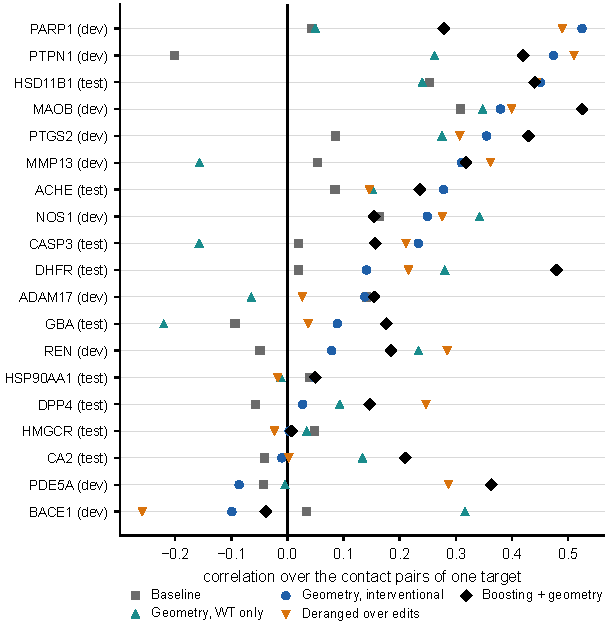
\includegraphics[width=0.7\linewidth]{figures/figS1_pertarget}
\caption{Correlation over the contact pairs of each held-out target for the baseline surrogates, the geometry network trained on wild-type scores, the geometry network trained on measured changes, the control with labels deranged over edits and the boosting model with geometry (seed ensembles). Targets are sorted by the correlation of the geometry network trained on measured changes; the role of each target is given in parentheses.}
\label{fig:si_pertarget}
\end{figure}

\begin{figure}[h]
\centering
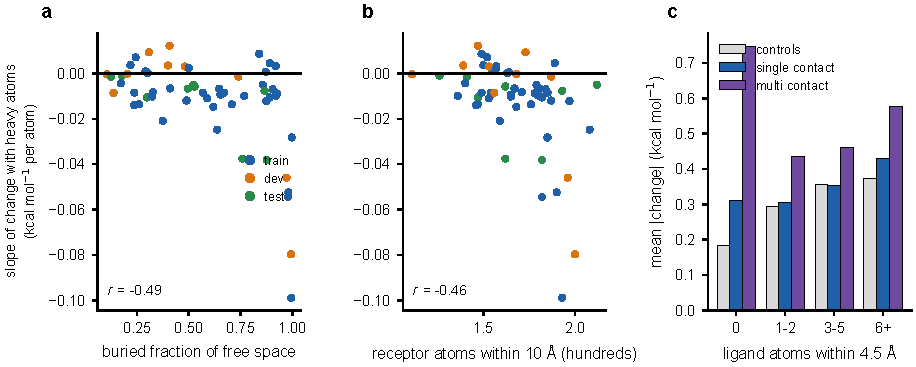
\includegraphics[width=\linewidth]{figures/figS2_law}
\caption{The size law and the pose dependence of the measured changes. (a) Slope of the change of the score with the heavy-atom count of the ligand against the buried fraction of free space, one point per target. (b) The same slope against the number of receptor heavy atoms within 10~\AA{} of the box center. (c) Mean absolute change against the number of ligand heavy atoms of the wild-type pose within 4.5~\AA{} of the removed side-chain atoms, for controls, single contact truncations and multi-residue truncations.}
\label{fig:si_law}
\end{figure}

\begin{figure}[h]
\centering
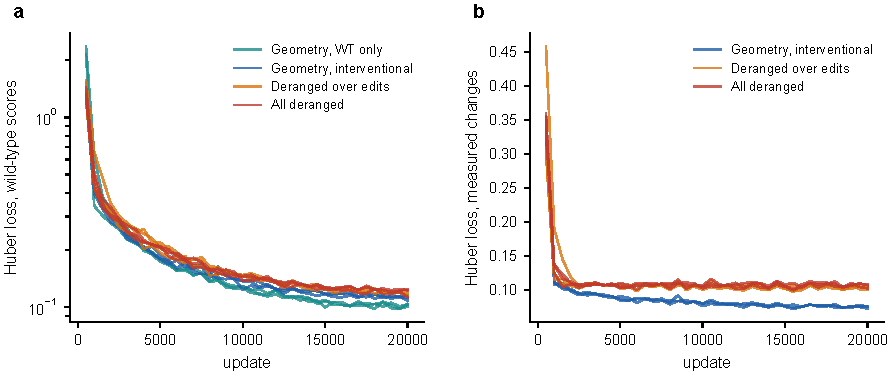
\includegraphics[width=\linewidth]{figures/figS3_curves}
\caption{Training curves of the registered conditions (seeds 11, 22 and 33). (a) Huber loss on wild-type scores. (b) Huber loss on measured changes; the level of the deranged controls marks the loss that labels without edit-specific information leave.}
\label{fig:si_curves}
\end{figure}

\end{document}
